%  LaTeX support: latex@mdpi.com 
%  For support, please attach all files needed for compiling as well as the log file, and specify your operating system, LaTeX version, and LaTeX editor.

%=================================================================
\documentclass[aerospace,article,submit,moreauthors,pdftex]{Definitions/mdpi} 

% For posting an early version of this manuscript as a preprint, you may use "preprints" as the journal and change "submit" to "accept". The document class line would be, e.g., \documentclass[preprints,article,accept,moreauthors,pdftex]{mdpi}. This is especially recommended for submission to arXiv, where line numbers should be removed before posting. For preprints.org, the editorial staff will make this change immediately prior to posting.

%--------------------
% Class Options:
%--------------------
%----------
% journal
%----------
% Choose between the following MDPI journals:
% acoustics, actuators, addictions, admsci, adolescents, aerospace, agriculture, agriengineering, agronomy, ai, algorithms, allergies, analytica, animals, antibiotics, antibodies, antioxidants, appliedchem, applmech, applmicrobiol, applnano, applsci, arts, asi, atmosphere, atoms, audiolres, automation, axioms, batteries, bdcc, behavsci, beverages, biochem, bioengineering, biologics, biology, biomechanics, biomedicines, biomedinformatics, biomimetics, biomolecules, biophysica, biosensors, biotech, birds, bloods, brainsci, buildings, businesses, cancers, carbon, cardiogenetics, catalysts, cells, ceramics, challenges, chemengineering, chemistry, chemosensors, chemproc, children, civileng, cleantechnol, climate, clinpract, clockssleep, cmd, coatings, colloids, compounds, computation, computers, condensedmatter, conservation, constrmater, cosmetics, crops, cryptography, crystals, curroncol, cyber, dairy, data, dentistry, dermato, dermatopathology, designs, diabetology, diagnostics, digital, disabilities, diseases, diversity, dna, drones, dynamics, earth, ebj, ecologies, econometrics, economies, education, ejihpe, electricity, electrochem, electronicmat, electronics, encyclopedia, endocrines, energies, eng, engproc, entropy, environments, environsciproc, epidemiologia, epigenomes, fermentation, fibers, fire, fishes, fluids, foods, forecasting, forensicsci, forests, fractalfract, fuels, futureinternet, futuretransp, futurepharmacol, futurephys, galaxies, games, gases, gastroent, gastrointestdisord, gels, genealogy, genes, geographies, geohazards, geomatics, geosciences, geotechnics, geriatrics, hazardousmatters, healthcare, hearts, hemato, heritage, highthroughput, histories, horticulturae, humanities, hydrogen, hydrology, hygiene, idr, ijerph, ijfs, ijgi, ijms, ijns, ijtm, ijtpp, immuno, informatics, information, infrastructures, inorganics, insects, instruments, inventions, iot, j, jcdd, jcm, jcp, jcs, jdb, jfb, jfmk, jimaging, jintelligence, jlpea, jmmp, jmp, jmse, jne, jnt, jof, joitmc, jor, journalmedia, jox, jpm, jrfm, jsan, jtaer, jzbg, kidney, land, languages, laws, life, liquids, literature, livers, logistics, lubricants, machines, macromol, magnetism, magnetochemistry, make, marinedrugs, materials, materproc, mathematics, mca, measurements, medicina, medicines, medsci, membranes, metabolites, metals, metrology, micro, microarrays, microbiolres, micromachines, microorganisms, minerals, mining, modelling, molbank, molecules, mps, mti, nanoenergyadv, nanomanufacturing, nanomaterials, ncrna, network, neuroglia, neurolint, neurosci, nitrogen, notspecified, nri, nursrep, nutrients, obesities, oceans, ohbm, onco, oncopathology, optics, oral, organics, osteology, oxygen, parasites, parasitologia, particles, pathogens, pathophysiology, pediatrrep, pharmaceuticals, pharmaceutics, pharmacy, philosophies, photochem, photonics, physchem, physics, physiolsci, plants, plasma, pollutants, polymers, polysaccharides, proceedings, processes, prosthesis, proteomes, psych, psychiatryint, publications, quantumrep, quaternary, qubs, radiation, reactions, recycling, regeneration, religions, remotesensing, reports, reprodmed, resources, risks, robotics, safety, sci, scipharm, sensors, separations, sexes, signals, sinusitis, smartcities, sna, societies, socsci, soilsystems, solids, sports, standards, stats, stresses, surfaces, surgeries, suschem, sustainability, symmetry, systems, taxonomy, technologies, telecom, textiles, thermo, tourismhosp, toxics, toxins, transplantology, traumas, tropicalmed, universe, urbansci, uro, vaccines, vehicles, vetsci, vibration, viruses, vision, water, wevj, women, world 

%---------
% article
%---------
% The default type of manuscript is "article", but can be replaced by: 
% abstract, addendum, article, book, bookreview, briefreport, casereport, comment, commentary, communication, conferenceproceedings, correction, conferencereport, entry, expressionofconcern, extendedabstract, datadescriptor, editorial, essay, erratum, hypothesis, interestingimage, obituary, opinion, projectreport, reply, retraction, review, perspective, protocol, shortnote, studyprotocol, systematicreview, supfile, technicalnote, viewpoint, guidelines, registeredreport, tutorial
% supfile = supplementary materials

%----------
% submit
%----------
% The class option "submit" will be changed to "accept" by the Editorial Office when the paper is accepted. This will only make changes to the frontpage (e.g., the logo of the journal will get visible), the headings, and the copyright information. Also, line numbering will be removed. Journal info and pagination for accepted papers will also be assigned by the Editorial Office.

%------------------
% moreauthors
%------------------
% If there is only one author the class option oneauthor should be used. Otherwise use the class option moreauthors.

%---------
% pdftex
%---------
% The option pdftex is for use with pdfLaTeX. If eps figures are used, remove the option pdftex and use LaTeX and dvi2pdf.

%=================================================================
% MDPI internal commands
\firstpage{1} 
\makeatletter 
\setcounter{page}{\@firstpage} 
\makeatother
\pubvolume{1}
\issuenum{1}
\articlenumber{0}
%\doinum{}
\pubyear{2021}
\copyrightyear{2020}
%\externaleditor{Academic Editor: Firstname Lastname} % For journal Automation, please change Academic Editor to "Communicated by"
\datereceived{} 
\dateaccepted{} 
\datepublished{} 
\hreflink{https://doi.org/} % If needed use \linebreak
%------------------------------------------------------------------
% The following line should be uncommented if the LaTeX file is uploaded to arXiv.org
%\pdfoutput=1

%=================================================================
% Add packages and commands here. The following packages are loaded in our class file: fontenc, inputenc, calc, indentfirst, fancyhdr, graphicx, epstopdf, lastpage, ifthen, lineno, float, amsmath, setspace, enumitem, mathpazo, booktabs, titlesec, etoolbox, tabto, xcolor, soul, multirow, microtype, tikz, totcount, changepage, paracol, attrib, upgreek, cleveref, amsthm, hyphenat, natbib, hyperref, footmisc, url, geometry, newfloat, caption

\usepackage[version=4]{mhchem}
\usepackage{gensymb}
\usepackage{textcomp}
%\usepackage[english]{babel}
%\usepackage{biblatex}
%\usepackage{amsmath}
\usepackage{graphicx}
%\usepackage{a4wide}
%\usepackage[left=2.25cm, right=2.25cm, top=3cm, bottom=2.5cm]{geometry}
\usepackage{fancyhdr}
\usepackage{url, lipsum}
%\usepackage{cleveref}
%\setcitestyle{numbers,comma,sort&compress,open={[},close={]}}
%\usepackage{cite}
\usepackage{wrapfig}
\usepackage{float}
\usepackage{multicol}
%\usepackage{pgfplots}
\usepackage{lscape}
\usepackage{tikz}
\usepackage{subcaption}
\usepackage{engord}
\usepackage{longtable}
\usepackage{graphicx}
\usepackage[normalem]{ulem}
\useunder{\uline}{\ul}{}
\usepackage{dblfloatfix}
%\pgfplotsset{width=10cm,compat=1.9}
\usepackage{multirow}
\usepackage{textcomp}
\usepackage{ragged2e}
\usepackage{csvsimple}
%\usepackage[citestyle=authoryear]{biblatex}
%\usepackage[center]{caption}
\usepackage{lastpage}
\usepackage{subcaption, setspace, booktabs}
\usepackage{enumitem}
\usepackage{nidanfloat}
\usepackage[labelfont=bf]{caption}
%\usepackage{mathptmx}
\usepackage{chngcntr}
\usepackage{titlesec}
\usepackage{hyperref}
%\usepackage[english]{babel}
\usepackage{blindtext}
%\usepackage{abstract}
%\usepackage[LGRgreek]
%\setcitestyle{numbers,comma,sort&compress,open={[},close={]}}

\usepackage[textwidth=4cm]{todonotes}
\reversemarginpar					% SB: so todo notes appear in left margin
\setlength{\marginparwidth}{0cm} 	% SB: this might muck up other layout stuff so remove if anything looks squiffy

\makeatletter
\newcounter{reaction}
%%% >> for article <<
\renewcommand\thereaction{R\arabic{reaction}}
%%% << for article <<
%%% >> for report and book >>
%\renewcommand\thereaction{C\,\thechapter.\arabic{reaction}}
%\@addtoreset{reaction}{chapter}
%%% << for report and book <<
\newcommand\reactiontag%
{\refstepcounter{reaction}\tag{\thereaction}}
\newcommand\reaction@[2][]%
{\begin{equation}\ce{#2}%
\ifx\@empty#1\@empty\else\label{#1}\fi%
\reactiontag\end{equation}}
\newcommand\reaction@nonumber[1]%
{\begin{equation*}\ce{#1}\end{equation*}}
\newcommand\reaction%
{\@ifstar{\reaction@nonumber}{\reaction@}}
\makeatother


%=================================================================
%% Please use the following mathematics environments: Theorem, Lemma, Corollary, Proposition, Characterization, Property, Problem, Example, ExamplesandDefinitions, Hypothesis, Remark, Definition, Notation, Assumption
%% For proofs, please use the proof environment (the amsthm package is loaded by the MDPI class).

%=================================================================
% Full title of the paper (Capitalized)
\Title{Aircraft Emissions, their Plume-Scale Effects, and the Spatio-Temporal Variability of the Atmospheric Response: a Review}
% The atmospheric response to aircraft emissions and the climate significance of plume-scale processing

% MDPI internal command: Title for citation in the left column
\TitleCitation{Aircraft Emissions, their Plume-Scale Effects, and the Spatio-Temporal Variability of the Atmospheric Response: a Review}

% Author Orchid ID: enter ID or remove command
\newcommand{\orcidauthorA}{0000-0000-0000-000X} % Add \orcidA{} behind the author's name
%\newcommand{\orcidauthorB}{0000-0000-0000-000X} % Add \orcidB{} behind the author's name

% Authors, for the paper (add full first names)
\Author{Kieran Tait $^{1,\dagger,\ddagger}$\orcidA{}, Firstname Lastname $^{1,\ddagger}$ and Firstname Lastname $^{2,}$*}

% MDPI internal command: Authors, for metadata in PDF
\AuthorNames{Kieran Tait, Firstname Lastname and Firstname Lastname}

% MDPI internal command: Authors, for citation in the left column
\AuthorCitation{Tait, K.; Lastname, F.; Lastname, F.}
% If this is a Chicago style journal: Lastname, Firstname, Firstname Lastname, and Firstname Lastname.

% Affiliations / Addresses (Add [1] after \address if there is only one affiliation.)
\address[1]{%
$^{1}$ \quad University of Bristol; kt16229@bristol.ac.uk\\
$^{2}$ \quad Affiliation 2; e-mail@e-mail.com}

% Contact information of the corresponding author
\corres{Correspondence: e-mail@e-mail.com; Tel.: (optional; include country code; if there are multiple corresponding authors, add author initials) +xx-xxxx-xxx-xxxx (F.L.)}

% Current address and/or shared authorship
\firstnote{Current address: Affiliation 3} 
\secondnote{These authors contributed equally to this work.}
% The commands \thirdnote{} till \eighthnote{} are available for further notes

%\simplesumm{} % Simple summary

%\conference{} % An extended version of a conference paper

% Abstract (Do not insert blank lines, i.e. \\) 
%\abstract{A single paragraph of about 200 words maximum. For research articles, abstracts should give a pertinent overview of the work. We strongly encourage authors to use the following style of structured abstracts, but without headings: (1) Background: place the question addressed in a broad context and highlight the purpose of the study; (2) Methods: describe briefly the main methods or treatments applied; (3) Results: summarize the article's main findings; (4) Conclusion: indicate the main conclusions or interpretations. The abstract should be an objective representation of the article, it must not contain results which are not presented and substantiated in the main text and should not exaggerate the main conclusions.}

% Keywords
\keyword{keyword 1; keyword 2; keyword 3 (List three to ten pertinent keywords specific to the article; yet reasonably common within the subject discipline.)} 

% The fields PACS, MSC, and JEL may be left empty or commented out if not applicable
%\PACS{J0101}
%\MSC{}
%\JEL{}

%%%%%%%%%%%%%%%%%%%%%%%%%%%%%%%%%%%%%%%%%%
% Only for the journal Diversity
%\LSID{\url{http://}}

%%%%%%%%%%%%%%%%%%%%%%%%%%%%%%%%%%%%%%%%%%
% Only for the journal Applied Sciences:
%\featuredapplication{Authors are encouraged to provide a concise description of the specific application or a potential application of the work. This section is not mandatory.}
%%%%%%%%%%%%%%%%%%%%%%%%%%%%%%%%%%%%%%%%%%

%%%%%%%%%%%%%%%%%%%%%%%%%%%%%%%%%%%%%%%%%%
% Only for the journal Data:
%\dataset{DOI number or link to the deposited data set in cases where the data set is published or set to be published separately. If the data set is submitted and will be published as a supplement to this paper in the journal Data, this field will be filled by the editors of the journal. In this case, please make sure to submit the data set as a supplement when entering your manuscript into our manuscript editorial system.}

%\datasetlicense{license under which the data set is made available (CC0, CC-BY, CC-BY-SA, CC-BY-NC, etc.)}

%%%%%%%%%%%%%%%%%%%%%%%%%%%%%%%%%%%%%%%%%%
% Only for the journal Toxins
%\keycontribution{The breakthroughs or highlights of the manuscript. Authors can write one or two sentences to describe the most important part of the paper.}

%%%%%%%%%%%%%%%%%%%%%%%%%%%%%%%%%%%%%%%%%%
% Only for the journal Encyclopedia
%\encyclopediadef{Instead of the abstract}
%\entrylink{The Link to this entry published on the encyclopedia platform.}
%%%%%%%%%%%%%%%%%%%%%%%%%%%%%%%%%%%%%%%%%%

\begin{document}

%%%%%%%%%%%%%%%%%%%%%%%%%%%%%%%%%%%%%%%%%%

\listoftodos

\input{Abstract.tex}
\section{Introduction}
Aircraft act as high-altitude emissions vectors, transporting a number of radiatively and chemically active substances across vast regions of the globe. These substances induce a net global warming effect that constitutes 3.5\% of global climate change due to anthropogenic emissions \cite{Lee2021}. Two thirds of this impact result from the climate forcing of non-\ce{CO_2} emissions, primarily through emission of nitrogen oxides (\ce{NO_x}), water vapour (\ce{H_2O}) and particulate matter (PM). These emission species interact with ambient air through chemical and microphysical processing, giving rise to the production and depletion of radiatively active substances that perturb the net energy balance of the atmosphere (e.g. \ce{NO_x}-induced ozone production, condensation trail (contrail) generation through \ce{H_2O} and PM emissions etc.). The degree to which aircraft emissions induce a climatic response varies depending on the state of the background atmosphere (i.e. its chemical composition and meteorology) and the time of day and year on which emissions are released. This means that aviation climate impact is spatio-temporally sensitive, i.e. the same emissions released at different times and/or locations can lead to very different climate effects. 

The dispersion of aircraft emissions occurs over great length and time scales, with emissions entrained in the aircraft exhaust plume which spreads hundreds of kilometres \cite{Kraabol2000a} over its lifetime of up to 12 hours \cite{EPA1992}. The elevated concentrations of emitted chemical species present within the plume result in additional nonlinear chemical (gas-phase and heterogeneous) and microphysical processes which are not accounted for in global chemistry models, due to the inherent assumption of instantaneous dispersion (ID) of emissions. The ID assumption models emissions as homogeneously mixed into the volume of the computational grid cell to which they are released, thus neglecting any subgrid-scale nonlinear processing that may occur throughout the plume lifetime \cite{Paoli2011}. Plume-scale nonlinear effects are also further augmented in high-density airspace regions, where plumes intersect and the emissions contained within them accumulate, leading to chemical saturation. Two key saturation effects have been noted to be of particular significance with respect to aviation climate impact: (1) the saturation of \ce{NO_x} emissions, which leads to decreasing ozone production with increasing \ce{NO_x} concentrations \cite{Jaegle1999}, and (2) the dehydration of water vapour leading to diminished contrail climate impact \cite{Schumann2015}. Therefore, the atmospheric response to non-\ce{CO_2} aircraft emissions is not only sensitive to natural variations in the atmospheric state, but it is also affected by heightened emissions concentrations due to the presence of lingering plumes from previous aircraft.

Optimising flight routes with respect to minimum climate impact (instead of minimum fuel burn) is a concept that has become prevalent in the literature in recent years. This involves re-routing aircraft to avoid particularly climate-sensitive regions of the atmosphere, based on provision of en-route chemical and meteorological information. Nikla{\ss} et al.\ (2019) \cite{Niklass2019} has shown through simulation efforts that it is possible to achieve a 12\% reduction in climate impact at virtually no additional cost to fuel burn, evidencing the practicability of climate-optimised routing. Other studies approach this issue purely from the perspective of superimposing aircraft plumes through formation flight. The aerodynamic benefits of formation flight due to wake energy retrieval are already well established \cite{Bangash2004, Kent2020}, however it has become increasingly evident that formation flight can also be used to exploit climate-beneficial saturation effects due to the superposition of plumes from aircraft involved. In Dahlmann et al.\ (2020) \cite{Dahlmann2020} a preliminary study exploring the potential for climate impact reduction due to saturation effects in formation flight and found that \ce{NO_x} saturation led to a reduction in ozone production efficiency of \textasciitilde5\% and a mutual inhibition of contrail growth, quelling their radiative properties by 20 to 60\%. 

This review article documents the current state of literature on aviation's atmospheric effects and the influence of nonlinear plume-scale processing on the global net climate impact, to bring to light the notion that aviation-induced perturbations to atmospheric chemistry can simply be viewed as another constraint in the climate-optimised routing problem. Section 2 covers the emissions generation process and the methods used to model aircraft performance and emissions. Section 3 explores the dispersion characteristics of aircraft emissions on the subgrid scale, alluding to the various modelling methods developed to investigate the dynamical characteristics of aircraft plumes. In section 4, air traffic management principles and their effect on aviation emissions distribution is considered, on both the local and global scale, followed by section 5 which explores aircraft climate impact, based on the emissions released and the chemical and physical processes that occur on the grid and subgrid-scale of global models. Section 6 looks into the effect of subgrid-scale processes that occur due to emissions accumulation in high-density airspace, and finally section 7 explores potential mitigation efforts to reduce aviation-induced climate change by modifying aircraft operations, such as climate-optimal routing and formation flight.


%This review article aims to bring together literature on these two concepts to prove that the
%This review article documents the current state of literature on aviation's atmospheric effects and the influence of nonlinear plume-scale processing on the global net climate impact, . Section 2 covers the emissions generation process and the methods used to model aircraft performance and emissions. Section 3 explores the dispersion characteristics of aircraft emissions on the subgrid scale, alluding to the various modelling methods developed to investigate the dynamical characteristics of aircraft plumes. In section 4, air traffic management principles and their effect on aviation emissions distribution is considered, on both the local and global scale, followed by section 5 which explores aircraft climate impact, based on the emissions released and the chemical and physical processes that occur on the grid and subgrid-scale of global models. Section 6 looks into the effect of subgrid-scale processes that occur due to emissions accumulation in high-density airspace, and finally section 7 explores potential mitigation efforts to reduce aviation-induced climate change by modifying aircraft operations, such as climate-optimal routing and formation flight.

%. Emissions of \ce{NO_x} indirectly affect the climate through photochemical reactions that generate ozone (\ce{O_3}) and deplete methane (\ce{CH_4}), leading to a net warming effect. In sufficiently cold and humid air, emitted water vapour condenses around PM to form water droplets, which subsequently freeze to form a trail of ice crystals in the aircraft wake. This is The formation of ice crystals in the aircraft wake constitutes what is known as a condensation trail (contrail). Contrails can grow due to uptake of surrounding water vapour and persist for hours, spreading over hundreds of kilometres of the atmosphere, with the possibility of transitioning into cirrus clouds known as contrail cirrus. Persistent contrails and contrail cirrus are known to trap heat more efficiently than they reflect inbound solar radiation, thus exhibiting a net warming effect, thought to be the most significant contribution to aviation-induced climate change \cite{Karcher2018}. 

%The dispersion of aircraft emissions occurs over great length and time scales, with emissions entrained in the aircraft exhaust plume which spreads hundreds of kilometres \cite{Kraabol2000} over its lifetime of up to 12 hours \cite{EPA1992}. The elevated concentrations of emission species present within the plume result in additional nonlinear chemical (gas-phase and heterogeneous) and microphysical processes which are not accounted for in global chemistry models, due to the inherent assumption of instantaneous dispersion (ID) of emissions. The ID assumption models emissions as homogeneously mixed into the volume of the computational grid cell to which they are released, thus neglecting any subgrid-scale nonlinear processing that may occur throughout the plume lifetime \cite{Paoli2011}. The inclusion of plume-scale modelling in the analysis of aviation climate impact captures the initial depletion of ozone in the plume due to the saturation of \ce{NO_x} emissions, followed by the conversion of \ce{NO_x} to nitrogen reservoir species (e.g. \ce{HNO_3}) on the order of 10\%, which are less efficient at producing ozone when propagated to global scales. The lack of accounting of these in-plume processes in the ID approach results in an overestimation of ozone forming potential by up to \textasciitilde20\% \cite{Fritz2020}. Furthermore, heterogeneous reactions that take place on aviation-induced aerosol particles in the plume can lead to the self reaction of a key oxidant known as the hydroperoxy radical (\ce{HO_2}), thus leading to further reduction of ozone production that is overlooked in global modelling efforts \cite{}. Insufficient microphysical modelling of contrails in aircraft exhaust plumes has also been shown to limit accuracy of climate impact calculations in global models \cite{}. The formation and persistence of contrails can be deduced purely from the satisfaction of thermodynamic criteria related to the saturation of ice and water in the surrounding atmosphere. However, determination of the evolution and radiative impact of contrails requires the microphysical analysis of key optical and physical properties, meaning the improper accounting of contrail and aerosol microphysics in global models leads to large uncertainties in the true global atmospheric impact of contrails \cite{}. 

%The ideal solution to the issue of inadequate accounting of subgrid-scale effects in global models would be to obtain high-resolution plume model data for every flight that takes place. In reality, flights take place in the hundreds of thousands every day, so the computational load from such a task would be exceedingly large \cite{}. Instead, plume models and large eddy simulations are used to deduce and calibrate parametrisations of these plume-scale processes, that can be applied to global models to capture the subgrid-scale effects without the need for full plume model implementation. Parametrisations of gas-phase conversions in the plume have been covered extensively in the literature, however the global modelling of heterogeneous chemistry and contrail microphysics is an area that is more difficult to approach, and work is still ongoing to reduce uncertainty in this area \cite{}.

%The degree to which nonlinear chemical and microphysical processing occurs in aircraft plumes varies with respect to temperature, time of emission, latitude, season, turbulence, and the background concentrations of key chemical species, primarily \ce{NO_x} and \ce{O_3} \cite{Kraabol2002}. This means that discrepancies between plume models and global models also deviate with location and time, and any attempts to parametrise plume processes into global models must take this spatio-temporal variability into account. The sensitivity of plume processes to environmental conditions also transfers to scenarios where multiple plumes overlap in high density airspace. The accumulation of emissions due to overlapping plumes in high-density airspace can lead to exceptionally high concentrations of key chemical species, with \ce{NO_x} and cloud condensation nuclei (CCN), such as soot and sulphate aerosol particles, expected to increase the most \cite{Brasseur1998, Schlager1997}. The perturbation to the chemical state of the atmosphere due to other aircraft emissions has been shown to have a considerable effect on the eventual climate impact of further emissions released, with the saturation of \ce{NO_x} leading to further reductions in ozone formation \cite{} and the dehydration of water vapour due to prior contrails leading to a diminishing effect of subsequent contrails released into the same volume of airspace \cite{}. Quantifying aviation's atmospheric impact on subgrid-scales therefore requires determination of the atmospheric state, and the integration of air traffic data, to deduce the perturbation of the atmospheric state due to prior flights through the same region of airspace.

%This review article documents the current state of literature on aviation's atmospheric effects and the influence of nonlinear plume-scale processing on the global net climate impact. Section 2 covers the emissions generation process and the methods used to model aircraft performance and emissions. Section 3 explores the dispersion characteristics of aircraft emissions on the subgrid scale, alluding to the various modelling methods developed to investigate the dynamical characteristics of aircraft plumes. In section 4, air traffic management principles and their effect on aviation emissions distribution is considered, on both the local and global scale, followed by section 5 which explores aircraft climate impact, based on the emissions released and the chemical and physical processes that occur on the grid and subgrid-scale of global models. Section 6 looks into the effect of subgrid-scale processes that occur due to emissions accumulation in high-density airspace, and finally section 7 explores potential mitigation efforts to reduce aviation-induced climate change by modifying aircraft operations, such as climate-optimal routing and formation flight.

%the distribution of air traffic and associated emissions on the global and local scale are . the climate impact of aviation, highlighting the global climate forcing, and how plume-scale processes play a part in this (section 5). 

%Air traffic literature shows that laws of minimum separation do not preclude the overlap of aircraft plumes \cite{}. In fact, in the scenario where two aircraft are pushed to their longitudinal separation minima, the follower aircraft's plume intersects the leader's in a matter of minutes \cite{}.

%Attempts to capture subgrid-scale effects in global models, without full integration of a high resolution plume model 
%To address the issue of inaccuracy in global aviation climate modelling efforts, various theories have been proposed to parametrise the chemical and microphysical effects occurring at the subgrid-scale.

%Parametrisation of gas-phase chemical conversions has been covered extensively in the literature, whereas 


%Just as the magnitude of aviation climate impact at a global scale depends on the time and location with which emissions are released, the degree to which plume-scale chemical and microphysical processing affects the eventual 

%The climate perturbation induced by nonlinear processing in aircraft exhaust plumes is again, entirely spatio-temporally dependent, meaning the

 %\ce{NO_x} to \ce{NO_y} conversion that takes place 

 %has been shown to reduce the net aviation-attributable ozone forming potential by up to \textasciitilde20\% \cite{Fritz2020}. This is because the conversion of \ce{NO_x} to nitrogen reservoir species (\ce{NO_y}) in the plume means that a proportion of \ce{NO_x} emissions are instead propagated to global scales as \ce{NO_y} species which are less efficient at producing ozone. 


%This is because the in-plume conversion of nitrogen oxides (\ce{NO_x}) to nitrogen reservoir species (\ce{NO_y}) is captured in plume models, which leads to  efficient at producing ozone when propagated to global scales \cite{}. Furthermore, the inclusion of heterogeneous chemical processes can further limit the production of ozone and reduce the conversion of \ce{NO_x} to \ce{NO_y} in atmospheric conditions conducive with persistent contrail formation, due to the dehydration and dehoxification of the surrounding atmosphere
%
%Aerosol particles  in the aircraft exhaust plume interact with emitted water vapour, leading to condensation, followed 
%
%Although aviation water vapour contributes a relatively small warming effect compared to other emission species, it does serve as a 
%
%The greenhouse effect due to aviation water vapour is a relatively small contribution to aviation-induced climate
%
%The climate contribution of aviation water vapour emissions is relatively small does have a small direct climate forcing due to the induced greenhouse effect, however its radiative impact predominantly derives from the formation of condensation trals 

%(1) the influence of nitrogen oxide (\ce{NO_x}) emissions on atmospheric ozone and methane concentrations and (2) the formation of ice clouds known as condensation trails (contrails) due to condensation of water vapour on  and heterogeneous freezing of water vapour on aerosol particles in the aircraft wake, and x


%The extent to which the ID assumption leads to loss of accuracy in global aviation climate modelling is 
%
%To address this lack of
%
%In the gas-phase, high levels of nitrogen oxides (\ce{NO_x}) in the plume locally deplete ozone (\ce{O_3}) levels, such that the eventual recovery in ozone production 
%
%the presence of the  nonlinear chemistry effects include more efficient conversion of nitrogen oxides (\ce{NO_x}) to nitrogen reservoir species in the plume, resulting in a net reduction in the ozone forming potential of \ce{NO_x} emissions compared to the equivalent released in an ID scenario.
%
%gas-phase chemical conversions of NOx to NOy in the plume which , thus
%
%The chemistry that 
%
%These nonlinear effects have a potentially significant influence on net climate impact, yet are not accounted for in global chemistry models due to the inherent assumption of instantaneous dispersion (ID) of emissions into the volume of the computational grid cell in which they are released into.  that neglects the sub-grid scale nonlinear processes that occur due to the enhanced concentrations of chemical species present in the exhaust plume throughout its lifetime \cite{Paoli2011}. 
% In high-density airspace, such as along the North Atlantic Flight Corridor, aircraft often fly in close proximity, giving rise to the superposition of their plumes and the accumulation of emissions contained within them \cite{Schlager1997}. 
%
%
%It has been shown in \cite{} that the overlap of four consecutive plumes can influence the nonlinear chemistry and microphysics significantly, leading to saturation effects that can potentially provide a net climate impact reduction.
%
%Following expulsion into the free atmosphere, aircraft exhaust species become entrained in the aircraft wake, forming a plume of elevated chemical concentrations which persist for 2 to 12 hours \cite{}, before fully dispersing into ambient air. The build-up of non-CO2 emissions in the plume give rise to a number of nonlinear chemical and microphysical effects, which influence the ensuing atmospheric response by altering the net production rates of radiatively active gases and affecting contrail formation and persistence. It is often the case however, that in large-scale atmospheric models, emissions are instantaneously diluted into the volume of the smallest resolved grid cell, with dimensions according to the model’s spatial resolution. The instantaneous dilution (ID) approach neglects the plume-scale processes, thus leading to discrepancies in the calculated climate response such as the overestimation of O3 production, CH4 and CO destruction, and the increased rate of NOx conversion to nitrogen reservoir species \ref{}. Furthermore, it is stated in \ref{} that the formation of ice in aircraft exhaust plumes may result in additional heterogeneous chemical reactions, that are not captured in global atmospheric models. 
%
%% Introduce each section and explain whats in them and how whole review pieces together and the purpose of the review
\section{Aircraft emissions}
\label{emissions}
Aircraft propulsion systems provide the essential driving force component to enable powerful and efficient flight. In modern commercial aviation, responsible for \textasciitilde88\% of global aviation fuel usage \cite{Gossling2020}, it is commonplace to use a gas turbine propulsion system operating on kerosene-based jet fuel. Aviation's environmental impact stems from the emission and dispersion of chemically and radiatively active substances that are generated during jet fuel combustion. This section details the emissions generation process and the modelling methods implemented to estimate emissions based on aircraft performance calculations and the determination of fuel consumption.

\subsection{The generation of aircraft emissions}
The widespread usage of kerosene-based jet fuels stems from the need to satisfy strict power-to-weight and safety requirements demanded by commercial aircraft; this is because kerosene has an exceptionally high energy density and wide operating temperature range at a low financial cost, compared with alternative fuel types \cite{Hemighaus2007, USDOE_2020}. The stoichiometric combustion of kerosene with air required to generate thrust, does however generate a number of chemically and radiatively active emission species which are emitted from the aircraft into its wake. These aircraft emissions interact with the surrounding atmosphere, perturbing the natural balance of chemistry and contributing to air quality issues and anthropogenic climate change. The mass of emission produced per unit mass of fuel burnt is often referred to as the emission index (EI), measured in grams of emission per kilogram of fuel [g/kg].

\subsubsection{Primary jet fuel combustion products}
The products of jet fuel combustion are often divided into two categories: primary and secondary, alluding to the way in which they are formed inside the aircraft engine. The primary products jet fuel combustion are carbon dioxide (\ce{CO_2}), water vapour (\ce{H_{2}O}) and, due to fuel impurities, a relatively small amount of sulphur oxides (\ce{SO_x}). These products are generated as a direct result of the combustion reaction that takes place, and hence depends on the carbon-hydrogen-sulphur composition of the fuel. The direct coupling of the production of these species to fuel consumption means that they have a constant EI throughout all phases of flight. Example values based on the typical chemical composition of jet fuel are given in table \ref{primary_EI_tab} \cite{IPCC1999}.

\begin{table}[H]
\centering
\caption{Emission indices estimates for \ce{CO_2}, \ce{H_2O} and \ce{SO_2}, averaged from a range of existing studies testing various aviation fuel types \cite{EUROCONTROL2001}.}
\begin{tabular}{@{}lll@{}}
\toprule
\textbf{\ce{CO_2}} & \textbf{\ce{H_2O}} & \textbf{\ce{SO_2}} \\ \midrule
3.149~g/kg fuel & 1.230~g/kg fuel & 0.84~g/kg fuel \\
\bottomrule
\end{tabular}
\label{primary_EI_tab}
\end{table}

\subsubsection{Secondary jet fuel combustion products}
Further to this, a number of secondary combustion products are generated in the aircraft exhaust, namely oxides of nitrogen (\ce{NO_x} = NO + \ce{NO_2}), carbon monoxide (CO), unburnt hydrocarbons (HC), particulate matter (PM) and trace levels of volatile organic compounds (VOCs) \cite{Brasseur1998}. These products are termed secondary, as their production levels differ depending on the nature of the combustion process and the engine load condition \cite{Deidewig1996}. This means that their EIs are variable throughout flight, depending on aircraft engine type, engine operating conditions, and the atmospheric conditions of the surrounding environment \cite{Dopelheuer2000}.
%IPCC chapter 7 ^
\ce{NO_x} emissions originate from the entry of atmospheric nitrogen (\ce{N_2}) into the high temperature combustion chamber. The level of \ce{NO_x} increases with increasing temperature and pressure, as it is coupled to the thermal reaction processes that occur in the primary combustion zone. Therefore, with the assumption of constant polytropic and combustion efficiencies, the emission index of \ce{NO_x} (EI\ce{NO_x}) can be correlated with aircraft fuel flow \cite{Dopelheuer1998, Deidewig1996}. As a result of inefficiencies in the combustion process, products such as CO and HC are formed. Contrarily to \ce{NO_x}, these emissions are direct products of incomplete combustion, meaning their concentrations are inversely proportional to combustion efficiency. Since combustion efficiency correlates with thrust for sea level static (SLS) conditions, and thrust correlates with fuel flow, this means that EICO and EIHC decrease with increasing fuel flow. 

PM emissions from aircraft can be categorised by their volatility: non-volatile PM (nvPM) and volatile PM (vPM). The primary source of nvPM present in aircraft exhaust is soot, which constitutes the greatest warming effect of all particles released from aircraft \cite{Gettelman2013}. Soot is generated in the fuel rich regions of the combustor, where the condensation of unburnt aromatic hydrocarbons takes place, converting low carbon content HC fuel molecules into carbonaceous agglomerates containing millions of carbon atoms \cite{Ebbinghaus2001, Bockhorn1994}. The extent of soot formation therefore depends on the fuel-air-ratio and the mixing processes that take place in the combustor, which vary with combustor design and are influenced by the non-homogeneous flow and temperature fields. Accurate measurements of these parameters are rare, making it very difficult to directly acquire quantitative data on soot emissions. Instead, soot EI can be estimated based on correlation with the so-called smoke number measured in engine certification procedures \cite{Dopelheuer1998}.

The formation of vPM from aircraft largely derives from the emission of sulphur derivatives, lubrication oil and VOCs \cite{Wayson2012}. During combustion, the sulphur content in the fuel is mostly oxidised to sulphur dioxide (\ce{SO_2}), some of which is then further oxidised to sulphuric acid (\ce{H_{2}SO_{4}}) when emitted into the atmosphere. In the presence of sufficient water vapour, sulphate aerosols (\ce{SO_4}) can be generated, which exhibit the largest cooling effect from aircraft PM emissions \cite{IPCC1999}. The sulphate EI is a factor of fuel sulphur content, which varies depending on fuel composition and the specific emissions characteristics of the engine \cite{Schumann2002}. Due to the low volatility of lubricant oil, the emitted oil vapour from aircraft will add to the condensed mass of VOCs and contribute to vPM concentrations. The VOCs produced either from the oxidized fuel fragments or due to the pyrolysis in the combustion chamber can also act as vPM, which may have sufficiently low vapour pressure to allow condensation in the atmosphere forming a coating on the surface of the nvPM, impacting cloud formation, precipitation and climate \cite{IPCC1999}. The particulate matter emitted near the exit nozzle plane of the combustor consists only of nvPM. However vPM are produced through nucleation and condensation downstream. Thus it is difficult to estimate the total amount of vPM produced within the exhaust plume, as the formation of vPM is dependent on the concentration of sulphates and VOCs present in the exhaust, and the distance from the combustor \cite{Masiol2014}.

% Schumann and Fahey IPCC 1999 chapter 3 ^

% Masiol figure here?

\subsection{Aircraft emissions modelling}
Accurate quantification of aircraft emissions for any given flight requires the calculation of aircraft performance to estimate the total energy consumed, and hence, the total fuel burnt throughout the flight duration. With knowledge of fuel flow rates experienced throughout flight, flow rates of aircraft emission species can be deduced based on empirical engine performance datasets and emissions models.

\subsubsection{Fuel burn estimation}
Computational modelling of aircraft performance allows the simulation of aircraft trajectories and the quantification of forces experienced throughout flight, enabling the approximation of thrust and fuel flow across all phases of flight. Aircraft performance models that are prevalent in academia and industry, such as the BADA (Base of Aircraft DAta) method \cite{Nuic2010} and Piano-X \cite{PIANO_X}, emulate aircraft behaviour by coupling a database of aircraft-specific performance datasets to mathematical models to calculate useful flight characteristics, such as fuel flow and fuel burn, at discrete time steps during flight. This iterative approach accounts for the time-varying nature of aircraft properties like mass, speed and heading, thus leading to a more accurate estimate of performance and fuel burn estimation. Further to this, models such as the Aviation Environment Design Tool (AEDT) \cite{AEDT} exist, which carry out four-dimensional (4-D) physics-based simulations of aircraft trajectories at an exceptionally high spatial and temporal resolution, providing highly accurate predictions of fuel consumption and localised emissions impacts. Such tools do however come at the expense of high computational and financial cost, and often require proprietary data that is unavailable to the public domain. An alternative state-of-the-art open-source performance model that has been made available in recent years is the OpenAP model \cite{Sun2020}. This model consists of four main components; the aircraft and engine property model, the kinematic and dynamic aircraft performance models, and utility libraries; and can describe the characteristics of 27 common aircraft and 400 turbofan engines, deeming it a feasible alternative for researchers who do not have access to proprietary data and licensing for the other more established models. 

\subsubsection{Calculating aircraft emissions at reference conditions}
Aircraft performance models provide estimates of aviation fuel burn, but to estimate the particular chemical speciation of emissions released due to fuel combustion, aircraft emissions models must be implemented. As mentioned previously, the primary combustion products, \ce{CO_2}, \ce{H_2O} and \ce{SO_2}, have a direct relation to the amount of fuel burnt and hence a constant EI for a given fuel composition, with standard estimates provided in table \ref{primary_EI_tab}. Secondary combustion products such as \ce{NO_x}, CO and HC however, largely depend on operational and atmospheric conditions. Empirical relationships between EI and fuel flow for secondary combustion products have been determined at reference operating conditions using engine performance datasets, such as the International Civil Aviation Organisation (ICAO) engine emissions databank \cite{ICAOEEDB}.  This databank was developed for the purpose of engine certification and compliance with landing and take-off (LTO) cycle emissions standards, outlined in ICAO Annex 16 Vol. II \cite{ICAO2008}. Engine test data have been collected at sea-level static (SLS), International Standard Atmosphere (ISA) conditions, for four reference operating conditions (thrust settings) relevant to the LTO cycle: take-off (100\% thrust), climb out (85\%), approach (30\%) and taxi in/out (7\%). For every engine at each of the four LTO modes, a reference fuel flow and corresponding emission index has been derived, allowing emissions to be estimated for aircraft operating under any of the four modes, to a reasonable degree of accuracy. An exemplary ICAO EI dataset is provided in table \ref{secondary_EI_tab}.

%As alluded to previously, the primary combustion products, \ce{CO_2}, \ce{H_2O} and \ce{SO_x} have a direct relation to the amount of fuel burnt and hence a constant EI for a given fuel composition, whereas the secondary products largely depend on operational and atmospheric conditions. Emissions of \ce{NO_x}, CO and HC can be correlated with fuel flow, meaning estimation of their emission indices requires knowledge of this relationship across the range of operating conditions experienced throughout flight. 



\begin{table}[H]
\centering
\caption{Example ICAO engine emissions data for Rolls Royce Trent 970-84 engine \cite{ICAOEEDB}.}
\begin{tabular}{lllll}
\hline
 & \textbf{Take-off} & \textbf{Climb out} & \textbf{Approach} & \textbf{Idle} \\ \hline
\textbf{Fuel flow {[}kg/s{]}} & 2.605 & 2.157 & 0.720 & 0.255 \\
\textbf{EI \ce{NO_x} {[}g/kg{]}} & 38.29 & 29.42 & 12.09 & 5.44 \\
\textbf{EI CO {[}g/kg{]}} & 0.32 & 0.31 & 1.16 & 13.38 \\
\textbf{EI HC {[}g/kg{]}} & 0.02 & 0.12 & 0.08 & 0.04 \\ \hline
\label{secondary_EI_tab}
\end{tabular}
\end{table}

\subsubsection{Calculating aircraft emissions at non-reference conditions}
In reality, aircraft spend the majority of flight outside of the LTO vicinity (above 3,000~ft), and the operating conditions and atmospheric conditions vary considerably. To enable the accurate analysis of aircraft emissions outside of reference conditions, a number of emissions modelling methods have been developed. Such methods apply the necessary adjustments and interpolations to the LTO-limited engine performance datasets, to generate more realistic estimates of aircraft emissions across the whole flight profile. SAE International Aerospace Information Report 5715 (AIR5715) \cite{AIR5715} describes a number of methods for calculating aircraft emissions throughout all modes of operation and compares their relative merits. For the primary combustion species, the Fuel Composition method is presented, which determines EI\ce{CO_2}, EI\ce{H_2O} and EI\ce{SO_x} from the proportions of carbon, hydrogen and sulphur in the fuel. The set of methods concerning the estimation of EI\ce{NO_x}, EICO and EIHC include the ICAO reference method, the Boeing fuel flow method 2 (BFFM2), the DLR fuel flow method and the P3T3 method, in order of increasing fidelity. The ICAO reference method serves as the simplest and least accurate approach, computing emissions purely based on the ICAO reference conditions, without applying corrections to account for atmospheric effects at altitude. Therefore, it is only applicable for emissions analysis of aircraft flying in the LTO region.  The remaining methods, BFFM2, DLR and P3T3 can be applied at all aircraft operating conditions, including at cruise, as they apply interpolations to engine performance datasets to determine emissions indices throughout the whole duration of a flight. The BFFM2 method and the DLR method (\ce{NO_x} only) are the mid-tier models, as they provide reasonable estimates of EIs purely from interpolating the EI reference data and applying corrections for atmospheric effects based on ambient meteorological data, aircraft fuel flow and Mach number. The gold standard for modelling of \ce{NO_x}, CO and HC emissions is however, the P3T3 method, as it utilises detailed thermodynamic modelling data to determine the precise emission indices at any given point throughout flight. Required data includes the combustor inlet temperature (T3), pressure (P3) and the fuel-air ratio (FAR) at both reference and operational conditions. All of which are difficult to obtain without access to proprietary engine-specific performance data, which limits the accessibility of this model to open-access researchers \cite{Brink2020, Dubois2006}.

See figure \ref{BFFM2} for an example of how EIs are interpolated based on the logarithmic relationship between EI and fuel flow, using the BFFM2 method \cite{Wasiuk2014}. Furthermore, methods are also presented to account for the remaining key emission species, such as the Derivative Factor method \cite{AEDT} used to approximate the EI values for VOCs such as non-methane HC (NMHC) throughout flight and the First Order Approximation method \cite{Wayson2012} used to estimate PM emission indices. The choice of method generally depends on the emission species to be observed, the compromise between modelling resources and data availability, and the level of accuracy required.

\begin{figure}[H]
  \centering
  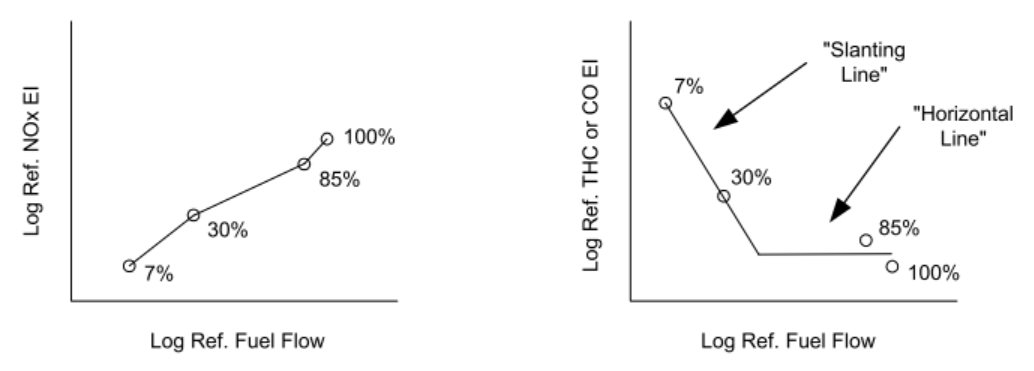
\includegraphics[width=0.9\linewidth]{BFFM2_output_example.png}
  \caption{Example log-log plots of EI against fuel flow at reference conditions, as prescribed by the BFFM2. The percentage values refer to the thrust as a percentage of maximum thrust at SLS conditions \cite{AIR5715}.}
  \label{BFFM2}
\end{figure}

\subsubsection{Emissions inventories and integration into large-scale climate models}
The estimation of aircraft emissions for a specific flight involves the simulation of aircraft performance across the entire flight profile so as to estimate fuel flow and engine operating conditions throughout flight. Knowledge of fuel flows and engine performance characteristics permits the estimation of aircraft emissions, based on the coupling of empirical engine certification data and emissions modelling methods, which interpolate the data to determine the emissions at non-reference conditions. This emissions estimation procedure is commonly carried out on a regional and global scale to determine emissions from a whole range of flights, which are then stored in so-called emissions inventories \cite{Wasiuk2016}. Aircraft emissions inventories collate data from all flights in the desired range and populate three-dimensional (3-D) latitude-longitude-altitude grid cells (e.g. 1\textdegree $\times$ 1\textdegree $\times$ 1000~ft) with total emissions quantities \cite{Paoli2011}. 

Aircraft emissions inventories are utilised to model the atmospheric effects of aviation, using large-scale atmospheric models that captures the chemistry, physics and dynamics of the Earth-atmosphere system (see section \ref{Climate_modelling} for further detail on climate modelling approaches). Such models allow one to simulate the perturbation to the state of the atmosphere due to an input of emissions and, in turn, provide quantitative indicators that enable modellers to determine the resultant climate impact (e.g. concentrations of key greenhouse gases, aerosol formation and distribution, cloud processes etc.) \cite{Jacobson2005}. However, one underlying issue with this conventional approach to aviation climate modelling, is that the use of gridded emissions data inherently assumes the instantaneous dispersion (ID) of emissions into the atmosphere \cite{Petry1998}. The ID approach assumes that aircraft emissions are instantaneously dispersed into the latitude-longitude-altitude computational grid cell in which they were released. The dimensions of this grid cell are solely determined by the spatial resolution of the global model, and hence do not serve as an accurate physical representation of emissions dispersion.

In reality, emissions released from aircraft are confined to the aircraft exhaust plume, which inhibits mixing with the surrounding atmosphere for up to a day after emission. Throughout this time, a number of nonlinear chemical and microphysical processes occur, due to the elevated concentrations of emissions species in the plume. These nonlinear plume-scale processes affect the eventual climate response to these emissions, yet most regional and global aviation climate impact studies \cite{Cariolle2009} often neglect the presence of the aircraft exhaust plume and opt for the simplified ID method. The following section explores the dynamical evolution of emissions following their release into ambient air, and discusses modelling approaches present in the literature which can be implemented to represent plume-scale effects in large-scale models. Such modelling is, however, often set aside due to computational issues associated with resolving consistency between the two model resolutions. 


%Throughout history, hydrocarbon fuels have been the dominant fuel source for aviation propulsion purposes, due to their unparalleled energy content and ease of availability.

%The allure towards fossil-based aircraft propulsion throughout the history of commercial aviation has resulted in grave environmental consequences, due to the harmful chemical species emitted into the atmosphere at aircraft cruising altitudes. 

%For an aircraft to achieve and maintain airborne status, it is required that the resistive force due to aerodynamic drag (D) and the gravitational force due to aircraft weight (W) are sufficiently overcome. The necessary driving force required to counteract drag and maintain forward speed is known as thrust (T). The forward speed induces airflow over the aircraft's cambered wings, thus rotating the flow downwards and generating lift (L) to counteract the aircraft weight. These constitute the four fundamental forces of flight \cite{Anderson1999}. The combination of these forces in varying magnitudes determines the trajectory of an aircraft and its instantaneous velocity and acceleration. The performance of an aircraft is highly dependent on the optimisation of the four forces, with structural configuration, material utilisation and payload affecting the aircraft’s weight, balance and stability, and the aircraft geometry affecting aerodynamics and hence influencing the lift and drag forces acting upon it. The thrust force however, is generated by means of a propulsion system. 
%
%\begin{figure}[H]
%  \centering
%  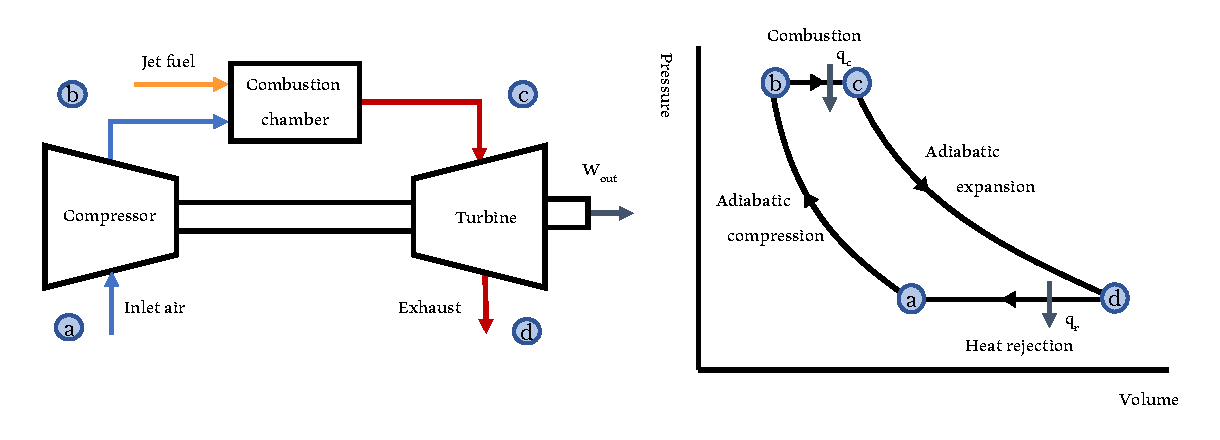
\includegraphics[width=1\linewidth]{Brayton.pdf}
%  \caption{The open-cycle Brayton thermodynamic cycle and its corresponding pressure-volume diagram, adapted from \cite{}.}
%  \label{Brayton}
%\end{figure}
%
%Traditional gas turbine engines, known as turbojet engines, employ the following four point Brayton thermodynamic cycle (see figure \ref{Brayton}): (a--b) the engine ingests oncoming air flow and passes it through a compressor, reducing volume and increasing total pressure; (b--c) the compressed air is mixed with fuel and ignited to cause a combustion reaction, with $q_c$ representing the heat addition to the system; (c--d) the high temperature, high pressure combustion products are passed through a turbine which extracts some energy from the flow to do work ($W_{out}$) to drive the compressor; (d--a) the airflow leaves the engine and is rejected into the atmosphere ($q_r$) at an accelerated rate through the exhaust nozzle. The magnitude of thrust generated by the engine is dependent on the mass of air being accelerated, and the difference in velocity of the air mass through the propulsion system \cite{Oates1989}. The commercial fleet of today primarily use bypass turbofan engines, which have an additional fan installed at the engine inlet. This fan is also powered by the turbine and its purpose is to bypass most of the intake air through the outer duct (often around \textasciitilde90\% according to modern day bypass ratios \cite{}. The addition of a bypass fan serves to increase the mass flow of air being accelerated by the engine, generating additional thrust without the need to burn additional fuel. This leads to a net increase in fuel efficiency of the engine compared to the turbojet equivalent, as the additional thrust generated due to the bypass design outweighs the additional fuel burn required to power the fan \cite{Richter2012}.




\section{The dispersion of aircraft emissions and the aircraft exhaust plume}
Following their expulsion into the free atmosphere throughout flight, aircraft exhaust gases are confined to a plume that undergoes a series of dynamical regimes (\textbf{jet}, \textbf{vortex}, \textbf{dispersion} and \textbf{diffusion} regimes), before becoming fully diluted in the surrounding air. The entrainment of emissions within the plume throughout these dynamical regimes leads to initial species concentrations that are several orders of magnitude higher than background levels \cite{Danilin1994}, giving rise to a number of nonlinear chemical and microphysical effects. These plume-scale effects have considerable implications on the eventual chemical composition of the surrounding atmosphere and lead to the formation of aerosols and ice crystals in the aircraft wake. Therefore, inclusion of plume-scale effects is vital for high fidelity modelling of aviation's impact on the climate. %A detailed description on the effect of plume-scale processes on the atmosphere, and the associated modelling practices can be found in section ... .

\subsection{Plume-scale dynamical regimes}
In order to accurately account for nonlinear effects experienced in the aircraft exhaust plume, one must first understand the dynamical response of the plume after combustion, to gauge the length and time scales over which aircraft emissions are entrained within it. 

\begin{figure}[H]
  \centering
  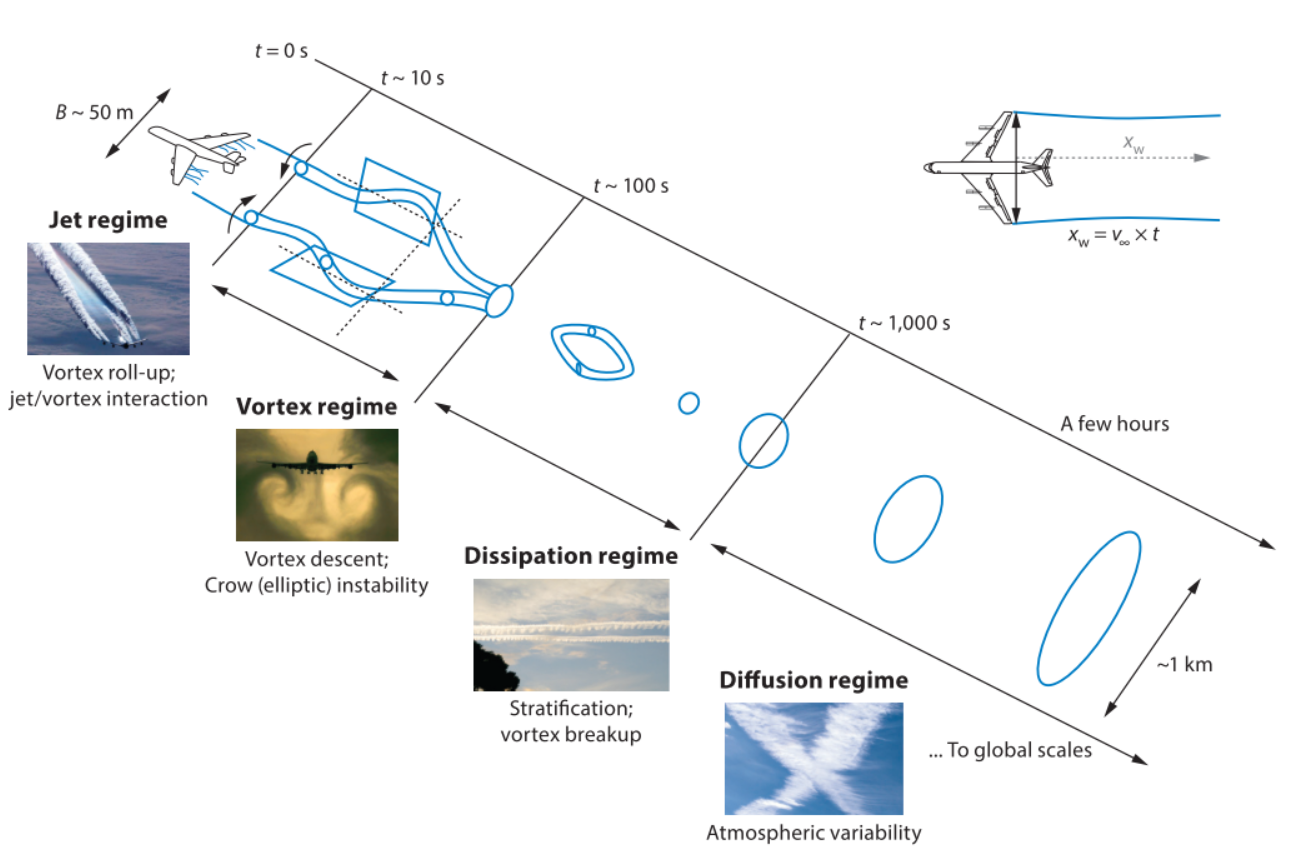
\includegraphics[width=0.8\linewidth]{Dynamics.png}
  \caption{Aircraft exhaust plume dynamical regimes. Wake distance behind aircraft $x_w = v_\infty \times t$ where $v_\infty$ is aircraft speed and $t$ is the post emission time \cite{Paoli2016, Gerz1998}.}
  \label{Plume}
\end{figure}

Exhaust gas temperatures range from around 1500~K post combustion, 600~K at engine tailpipe, followed by mixing with bypass air cooling the flow to around 300~K \cite{Brasseur1998} as the dispersion process begins. During the first 1--20~s post emission, an axisymmetric jet is formed, which rapidly diffuses into ambient air and cools to ambient temperatures. Over this period, known as the \textbf{jet} regime, the airflow passing over the wings is diverted downwards to generate lift, thus creating a vortex sheet at the trailing edge of the aircraft. This vortex sheet rolls up into a pair of counter-rotating vortices which are shed at the wing tips. The evolving vortex pair then merge together and propagate downwards, due to their mutually induced downwash velocity, trapping the exhaust plume within their cores and signalling the beginning of the vortex regime.

Throughout the \textbf{vortex} regime, which occurs between 20~s and 2 minutes after combustion, the primary wake containing the vortices and trapped exhaust plume sinks by around 150--200~m, resulting in a slight temperature increase of 1--3~K, due to the adiabatic heating of exhaust constituents in the sinking vortices. Further to this, the organised vortical structure means the wake does not grow significantly during this time, and hence the concentrations of entrained chemical species remain relatively constant. The adiabatic heating of the exhaust does however lead to baroclinicity at the border between each vortex and the ambient air, which detrains some momentum, heat and exhaust constituents from the primary wake, to form a secondary wake. This secondary wake trails upwards as it is warmer than the surrounding ambient air, and it escapes the influence of the vortex structure, resulting in enhanced mixing with ambient air and thus experiences different chemical and microphysical processes compared with the primary wake \cite{Gerz1998}.

Following this is the \textbf{dispersion} regime, in which the aircraft-induced dynamics subside due to the growth of Crow instability \cite{Crow1970}, which dissipates and disintegrates the primary and secondary wake vortices \cite{Paoli2016}. The breakdown of the organised vorticial structure and the production of turbulent motion leads to a sudden increase in the rate of entrainment between the exhaust plume and the ambient air by a factor of 10, therefore giving rise to a continuous decay of concentration and temperature within the plume. This regime lasts for 2--5 minutes after combustion, however this varies as the strength of aircraft induced vortices is proportional to the weight and span, and inversely proportional to the speed of the aircraft \cite{Gerz1998}

Lastly, the plume undergoes its final dynamical event, known as the \textbf{diffusion} regime. This regime is characterised by the aircraft-induced dynamics becoming negligible (after about 6 minutes \cite{Unterstrasser2014}), followed by the subsequent dominance of atmospheric processes in the spreading of the aircraft exhaust plume and its constituents. Atmospheric turbulence, radiation transport and stratification are examples of natural phenomena that contribute to the diffusion of the plume, with total dilution to ambient concentrations often occurring over timescales of 2--12~h post emission \cite{EPA1992}. During this time, the plume may spread up to a few kilometres through atmospheric turbulence and shear in the ambient air, diluting the exhaust species over vast volumes of airspace \cite{Schumann1995}.

Plume-scale climate effects that result from the confinement of emissions to the aircraft exhaust plume during the four dynamical regimes considerably alter the eventual global warming effect of a particular flight, and therefore should be appropriately accounted for in modelling efforts to estimate aviation's climate impact.

\subsection{Plume-scale modelling}
To tackle the issue of neglected plume-scale effects in the computational analysis of aviation-induced climate change, a number of plume modelling methods of varying fidelity have been theorised in the literature. Sub-grid resolution plume models simulate the dynamical response of the aircraft plume, so as to capture the nonlinear chemistry and microphysical effects that occur within it. The outputs of plume models can then be parametrised into low-resolution global models, to increase the accuracy of climate impact calculations through better accounting of the emissions dispersion process. 

\subsubsection{Empirical dilution model}
Plume dynamics control the rate at which aircraft emissions mix and dilute into the surrounding atmosphere, directly affecting the resulting climate impact of aircraft emissions due to the nonlinear effects experienced in the plume, before it becomes homogeneously mixed into the ambient air. Quantifying the rate of dilution and modelling the climate effects that occur within aircraft plumes is therefore an essential process in the accurate analysis of aviation's climate impact \cite{Schumann1995}. In Schumann et al. (1998) \cite{Schumann1998}, an empirical dilution model was developed to investigate the mixing rate of plumes throughout their typical lifetimes, based on data collated from over 70 aircraft exhaust plume encounters with research aircraft. The characteristic property observed in this study is the plume dilution ratio, $N$, which is defined as the amount of air mass that the exhaust plume generated from a unit mass of fuel burn, mixes with, per unit flight distance within the bulk of the plume. 

\begin{figure}[H]
 \centering
 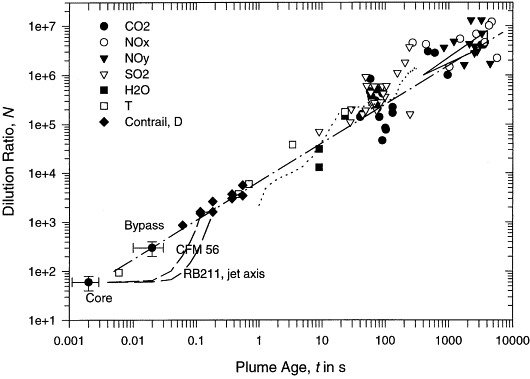
\includegraphics[width=0.75\linewidth]{Schumann_fig.jpg}
 \caption{Dilution ratio against plume age derived from empirical data. Marker shapes correspond to tracer species as displayed in legend. Markers with error bars correspond to characteristic values for the engine core (leftmost and lower) and bypass exits (rightmost and upper). The dashed curves near the core represent dilution on the jet axis, calculated for two engine types: CFM56 and RB211. The dotted curve represents large eddy simulation results from Gerz and Ehret (1997) \cite{Gerz1997}. The range of dilution values computed for large plumes ages by D{\"u}rbeck and Gerz (1996) \cite{Durbeck1996} are bounded by the triangle, top right of the figure. The dash-dotted line shows the interpolation that is represented by equation \eqref{N_equation} \cite{Schumann1998}.}
 \label{Schumann_dilution}
 \end{figure}

In figure \ref{Schumann_dilution}, measured dilution ratios from the plume encounters are plotted against plume age. The data was generated by measuring the concentrations of a range of chemical sources across a variety of aircraft types, within the time interval of 0.001--10,000~s. The significance of these findings is that, in spite of the diverse range of chemical species and aircraft types observed, throughout all four dynamical regimes, a relatively consistent logarithmic relationship emerges between dilution ratio and increasing plume age. When interpolating the regression line fitted to the data in figure \ref{Schumann_dilution}, the following equation can be obtained where $N$ represents dilution ratio, $t$ is plume age in seconds, and $t_0$ serves as an arbitrary reference scale.

\begin{equation}
	N = 7000(t/t_0)^{0.8}, \; 	t_0 = 1~s 
	\label{N_equation}
	\end{equation}
	
It is evident from the figure however, that encounters with plumes older than 50--100~s tend to diverge from the line fit, indicating a reduction in accuracy of the logarithmic approximation over time. This is likely due to the transition from the organised vortex structure present in the vortex regime, to the turbulent dispersion regime, where more unpredictable atmospheric processes begin to take place and become the primary influence on the evolution of the plume. Therefore, this empirical model can only be used reliably up to the vortex regime. Beyond this, a Gaussian approximation to the distribution of species concentrations is typically employed, accounting for dispersion effects experienced at cruising altitudes, such as advection, gravitational sedimentation, anisotropic diffusion, wind shear and stable stratification \cite{Konopka1995}. Two popular modelling methods which implement Gaussian approximation and the two-dimensional diffusion equation to model aircraft plumes over their whole lifetime are the Single Plume model and its discretised counterpart, the Multi-layered Plume model.

\subsubsection{Single and Multi-layered Plume models}
The Single Plume (SP) model, first presented in Petry et al. (1998) \cite{Petry1998}, approximates the time-evolving concentration field of an aircraft exhaust plume using a Gaussian distribution \cite{Vohralik2008}. Petry represents diffusion through eq. \eqref{diffCi}, a differential equation that describes the temporal variation of exhaust concentration $C$ of species $i$ in the plume

\begin{equation}
	\frac{\partial C_{\mathrm{i}}}{\partial t} = -sz \frac{\partial}{\partial y} C_{\mathrm{i}} + D_{\mathrm{v}} \frac{\partial^2}{\partial^2 z} C_{\mathrm{i}} + D_{\mathrm{h}} \frac{\partial^2}{\partial^2 y} C_{\mathrm{i}} + 2D_{\mathrm{s}} \frac{\partial^2}{\partial y \partial z} C_{\mathrm{i}}
	\label{diffCi}
\end{equation}

This two-dimensional diffusion equation is a function of wind shear ($s$), horizontal ($y$) and vertical distance from plume centre ($z$), and the horizontal ($D_{\mathrm{h}}$), vertical ($D_{\mathrm{v}}$) and shear ($D_{\mathrm{s}}$) diffusion coefficients, as calculated based on empirical data recorded under typical atmospheric conditions at aircraft cruising altitudes and assuming a horizontal flight path \cite{Durbeck1995}. The solution to the diffusion equation is a time-varying Gaussian function, with standard deviations $\sigma_{\mathrm{h}}$, $\sigma_{\mathrm{v}}$ and $\sigma_{\mathrm{s}}$ that depend on $s$, $D_{\mathrm{h}}$, $D_{\mathrm{v}}$, $D_{\mathrm{s}}$, time $t$ and the respective initial values ${\sigma_{\mathrm{0h, v}}}^2$


\begin{align}
\begin{split}
	{\sigma_{\mathrm{h}}}^{2}(t) {}&= \frac{2}{3} s^2 D_{\mathrm{v}} t^3 + (2 D_{\mathrm{s}} + s {\sigma_{\mathrm{0v}}}^2) s t^2 + 2 D_{\mathrm{h}} t + {\sigma_{\mathrm{0h}}}^2,
\end{split} \\
\begin{split}
	{\sigma_{\mathrm{v}}}^{2}(t) {}&= 2 D_{\mathrm{v}} t + {\sigma_{\mathrm{0v}}}^2,
	\end{split}\\
	{\sigma_{\mathrm{s}}}^{2}(t) {}&= s D_{\mathrm{v}} t^2 + (2 D_{\mathrm{s}} + s {\sigma_{\mathrm{0v}}}^2) t.
\end{align}

The standard deviations of the Gaussian function can then be used to deduce useful parameters such as plume cross-sectional areas and concentrations. Outputs such as these can serve as input to atmospheric models, enabling the simulation of the dynamical evolution of the plume, and its entrained emissions throughout its lifetime. 

The main drawback of the SP model however, is the assumption of homogeneous concentration distribution throughout the plume at any given time. This homogeneity assumption is sufficiently accurate up to the vortex regime, where plume cross-sectional areas are relatively small, entrainment rates are low, and the mixing ratio is relatively consistent across the plume diameter \cite{Fritz2020}. However, beyond this, the spike in entrainment rates following the breakdown of vortices causes rapid plume expansion, and the drop in concentration from plume core to outer edges becomes increasingly significant \cite{Meijer2001, Melo1978}. This spatial concentration gradient along the plume cross-section cannot be captured using the SP approach, so an alternative model is proposed, known as the Multi-layered Plume (MP) model, as seen in figure \ref{MP_model}. The MP model builds upon the SP model by discretising the plume cross-section into a number of concentric rings, enabling the inhomogeneous concentration profile to be represented by varying the mean concentration in each ring.

\begin{figure}[H]
 \centering
 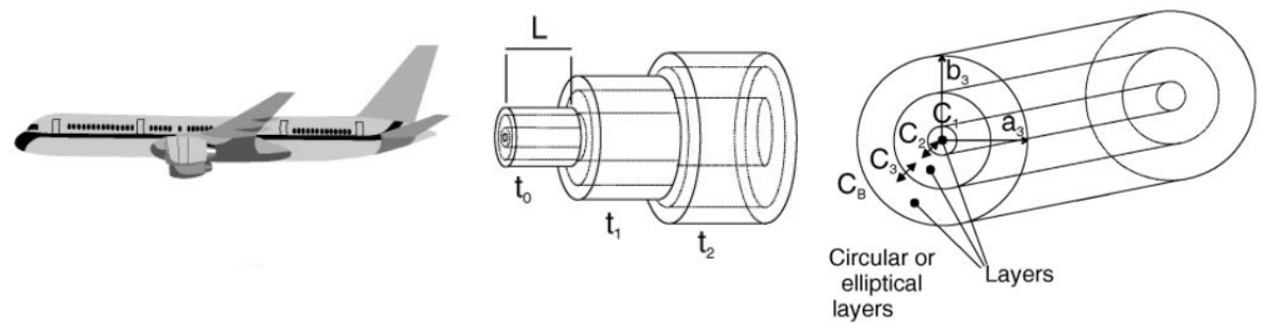
\includegraphics[width=0.9\linewidth]{MP_model.png}
 \caption{MP model visual representation \cite{Kraabol2000a}. Plume length L was set to the distance travelled over 1 s (247 m in this scenario) with three out of eight concentric rings shown for each timestep. $C_1 - C_3$ indicate the concentrations in each ring and the arrows represent mixing between the layers.}
 \label{MP_model}
 \end{figure}

As Kraabol et al.\ (2000a) \cite{Kraabol2000a} states, the Gaussian approximation to emissions dispersion only applies to the dynamical evolution of passive species, and is not suitable for modelling the evolution of chemically active species, due to the nonlinear chemical response in the plume. To counteract this issue, this paper implements an adapted version of the MP model, in which the plume is divided into 8 concentric rings, each with a chemistry module incorporated to estimate the chemical production and loss mechanisms of all species present. Applying this model under assumed turbulent conditions derived from D{\"u}rbeck and Gerz (1996) \cite{Durbeck1996}, graphs of horizontal and vertical plume radius are plotted against plume age, as shown in figures \ref{Kraabol}. After just 1 hour, it is predicted that plumes can spread between 1 and 10~km horizontally, whilst only reaching around 50--100~m vertically due to atmospheric stratification \cite{Durbeck1995}. As the plume approaches the end of its typical lifetime, between 10 and 15~h, plume cross-sections can reach 100--200~km horizontally and 200--400~m vertically. The vast length scales over which plumes span throughout their lifetime provides ample evidence to suggest that, in high-density airspace, plumes can overlap. The overlapping of plumes can thus lead to spikes in emissions concentrations that exceed that of single aircraft plumes, thus augmenting nonlinearities in the climate response and further propagating discrepancies between plume and global model outputs \cite{Schlager1997}. 


\begin{figure}[H]
	\centering
	\subfloat
		{
\centering
		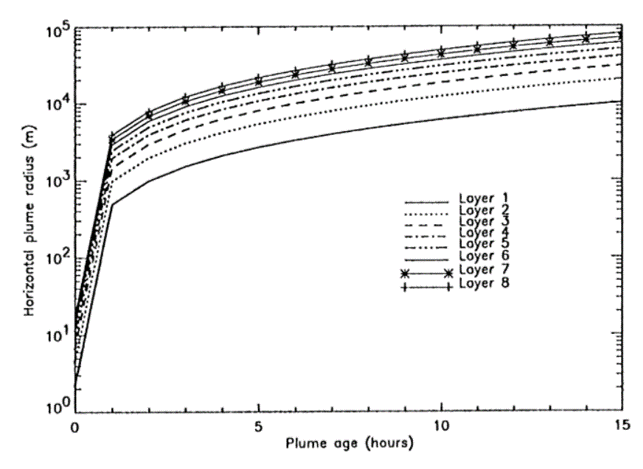
\includegraphics[width=.36\textwidth]{Kraabol1.png}
		}
	\subfloat
		{
\centering
		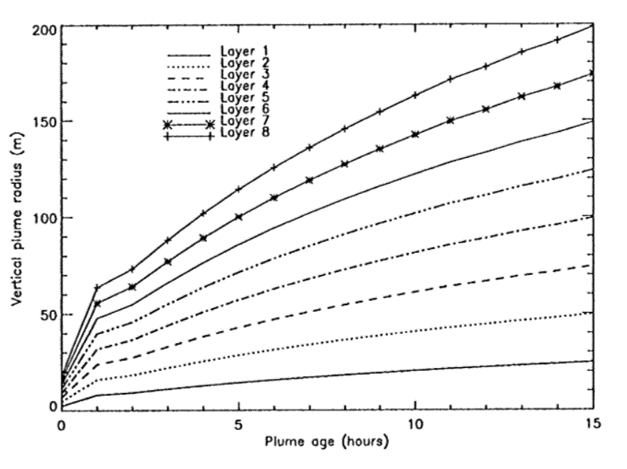
\includegraphics[width=.36\textwidth]{Kraabol2.png}
		}
	\caption{Evolution of \textbf{(a)} horizontal and \textbf{(b)} vertical plume radius over time, for MP model under assumed turbulent conditions \cite{Kraabol2000a}.}
	\label{Kraabol}
\end{figure}

\subsubsection{Aircraft Plume Chemistry, Emissions, and Microphysics Model (APCEMM)}
Models such as APCEMM from Fritz (2018) \cite{Fritz2018} further increase the accuracy of the SP and MP models by capturing additional effects that affect plume evolution and hence the resultant climate response once the plume is fully diluted. This includes effects such as plume anisotropy and asymmetry which impact the eventual spatial distribution of the plume, and modelling of the microphysical processes that strongly influence contrail formation and persistence. The model is similar to the MP model in that a chemistry module is simulated in a number of concentric rings which have differing concentration fields, that decrease with increasing radial distance from the plume core. The rest of the computation (i.e. mixing and microphysics) is peformed on a high-resolution Cartesian grid \cite{FritzConvo}. The primary aim of this model development was to bridge the gap between the simplified Gaussian approximation and more comprehensive large eddy simulations, as elaborated on in the following subsection.

% Figure??

\subsubsection{Large eddy simulations (LESs)}
Finally, the plume dynamical evolution can be most accurately captured using high-resolution LESs over the entire lifetime of the plume. LESs can model dynamics on a scale of several millions of grid points for a few seconds to a few minutes of plume age, providing unmatched levels of accuracy at the cost of extremely high computational demand. For this reason, LESs are usually limited to case studies from which the data obtained can be used to derive and calibrate plume parametrisations for use in the lower fidelity methods \cite{Lewellen1998}. 

In D{\"u}rbeck and Gerz (1995) \cite{Durbeck1995}, LES data are used to calculate effective diffusion coefficients and plume cross-sectional properties for plume modelling purposes. The data obtained from the simulations is said to have agreed with Schumann et al.\ (1995) \cite{Schumann1995}, where the horizontal and vertical plume scales and respective diffusivities are estimated from experimental data captured by a research aircraft measuring NO concentrations. Moreover, LESs have been used to determine plume properties on much shorter timescales in Unterstrasser et al.\ (2014) \cite{Unterstrasser2014}. In this paper, plume evolution is analysed for the jet and vortex period up to 6 minutes, whilst aircraft-induced dynamics dominate; concentration profiles and plume cross-sectional areas are determined for a range of atmospheric conditions, varying stratification, turbulence, wind shear and aircraft properties. Similarly in Paoli (2008) \cite{Paoli2008}, detailed LES numerical simulations are carried out for the jet and vortex phase, confirming hypotheses surrounding aerosol and microphysics modelling. These studies exemplify the use of LES methods to validate experimental findings, and serve as a means of calibration for plume model parameters that represent real-life plume dilution characteristics.


% Despite the extraordinary level of detail LES models are capable of achieving with current computational capabilities, issues still arise when attempting to integrate high resolution plume models into coarse global and regional atmospheric models, due to difficulties in resolving consistencies between the two models. To 


%\subsubsection{Plume lifetime}
%The lifetime of a plume is typically signified by the end of the diffusion regime and eventual return towards ambient background concentrations, around 2--12 h post emission. However, numerous distinct definitions have become apparent over the past few decades, which enable the concept of plume lifetime to be measured and used to determine the duration over which plume-scale processes should be accounted for when modelling the atmospheric effects of aviation. In \cite{Paoli2011}, three definitions of plume lifetime are explored. 
%
%The first of these is the so-called ``dispersion'' time ${t_{ref}}$ \cite{Petry1998}, defined as the time it takes for the plume to occupy the dimensions of a given reference area ${A_{ref}}$. This can be a useful metric to determine the time taken for a plume to become fully immersed in a known volume such as a latitude-longitude grid box of a global atmospheric model or the boundaries of a flight corridor. The second definition of plume lifetime is known as the ``mixing'' time ${t_{mix}}$, as  \cite{Karol2000, Kraabol2000, Meijer2001}. This is the time in which the chemical conversion rate of \ce{NO_x} in the plume becomes sufficiently close to that of the surrounding ambient air, falling below a very small threshold value. The dependency on the state of the background atmosphere means that this lifetime can change significantly with time and location. The final definition is from \cite{Cariolle2009} where the lifetime ${t_l}$ is determined by the exhaust concentrations dropping below a threshold mixing ratio and the excess exhaust mass dropping to zero. 
%
%The second lifetime definition, ${t_{mix}}$, is entirely dependent on the state of the background atmosphere, meaning the lifetime is subject to change significantly given a change in time and/or location of emission, as shown in figure 1 of \cite{Karol2000}. Moreover, the first and third definitions not only vary with atmospheric conditions, but also depend on the threshold values set by the observer, meaning consistent thresholds must be maintained throughout a given study to maintain validity. Results from the aforementioned studies produced estimates of plume lifetime that lie in the range of 10--20 h. Given that plume lifetime and rate of mixing are calculable and measurable concepts, it is now possible to model the temporal and spatial scales of the chemically active plume, so as to investigate the extent to which nonlinear chemistry and microphysics influence the ensuing climate impact throughout the lifetime of the plume.#

%\subsection{Aircraft plume characteristics}
%The entrainment of aircraft emissions into the exhaust plume following release into the atmosphere has a considerable effect on the ensuing climate response, through nonlinear chemical and microphysical processing. The magnitude of plume processing is influenced by the spatial and temporal characteristics of the plume. This means that quantitative assessment and modelling of plume-scale effects on the climate requires knowledge of key plume properties such as the characteristic rate of mixing with ambient air, throughout the 4 dynamical regimes, and the lifetime over which the plume typically resides.



\section{Air traffic and emissions distribution}
The previous section discussed the forces of flight and the generation and dispersion of aircraft emissions, from the perspective of a single aircraft. However, the state of the atmosphere is inhomogeneous with respect to space and time, meaning that the climate sensitivity to aircraft emissions differs considerably, depending on the time and location of their release. Furthermore, in airspace regions where traffic density is high, aircraft fly in close proximity and their exhaust plumes may intersect, giving rise to nonlinear local climate effects that must also be considered in aviation climate analysis. Therefore it is useful to explore the influence of air traffic management and spatial and temporal demand on the distribution of air traffic, and hence its associated emissions. 

\subsection{Air traffic management}
Air traffic management (ATM) is the system of services responsible for overseeing the network-wide implementation of safe, orderly and efficient air traffic flows, providing assistance to aircraft in transit from departure to destination aerodrome. It is the role of the air traffic control (ATC) team to manage and monitor air traffic in their respective airspace in real time, ensuring that optimum safety, order and efficiency of aircraft operations are maintained at all times \cite{SecretariatGeneral2016}. 

%This means that air traffic controllers must constantly monitor the state of the airspace, swiftly identifying and resolving any unfavourable circumstances by issuing the appropriate clearances or instructions to rectify the situation. 

\subsubsection{Air traffic safety} 
The inherent risk involved in the transportation of vast numbers of passengers at near transonic speeds through the upper atmosphere means that aviation safety is of paramount importance. A safe aircraft operation takes the path of least danger, primarily influenced by the need to avoid unfavourable atmospheric conditions and to prevent conflicts with other aircraft \cite{Zhang2012, Baumgartner2007}. In-flight atmospheric conditions susceptible to icing, turbulence or the presence of hazardous convective weather can all be classified as unfavourable for aircraft, with the latter presenting the greatest constraint on aircraft routing \cite{Mitchell2006, Krozel2007}. The increased risk resulting from flight through weather-affected regions means that aircraft must re-route, leading to restrictions on available airspace and deviations from the optimal flight profile, thus increasing flight-times, fuel burn and delays \cite{weather_delay_2021}.

The safety risks associated with aircraft-to-aircraft collisions necessitate air traffic controllers to impose safe separation standards between aircraft in the lateral, longitudinal and vertical direction, as specified in \cite{ICAOPANSDoc44442016}. The stated minimum separation distances between aircraft are 5 nautical miles (NM) laterally, 20 NM longitudinally and 1,000 ft in the vertical direction under the most lenient scenarios. A breach of separation laws in more than one direction is known as a conflict and must be resolved as quickly as possible. The enforcement of separation minima therefore introduces a theoretical upper limit on airspace density, i.e. the number of aircraft that occupy a fixed volume of airspace at any one time. 

\subsubsection{Air traffic order} 
To keep air traffic flows organised within controlled airspace, aircraft are ordered to follow the traditional fixed-route air traffic network, constructed from four key airspace elements that facilitate the air traffic management process \cite{SecretariatGeneral2016}:

\begin{itemize}
\item \textbf{airports/aerodromes} - an area of land or water intended to be used for the arrival, departure and surface movement of aircraft;
\item \textbf{waypoints} - a specified geographical location used to define the flight path of an aircraft, representing either a navigational aid (navaid) or a reference coordinate that the aircraft must fly by or fly over;
\item \textbf{airways} - a controlled portion of airspace established in the form of a corridor (usually 8-10NM wide) between two waypoints;
\item \textbf{sectors} - a region of airspace managed by a single ATC team, stratified into various levels to accommodate a wide variety of traffic.
\end{itemize}

In \cite{Odoni1987}, the notion of optimising air traffic flows for a given demand and capacity is explored, in which air traffic flows are represented using these four key elements. \textbf{Airports} represent the sources and sinks of the flow, \textbf{airways} are the arcs along which the flow travels, \textbf{waypoints} are the network nodes at which airways intersect, merge or diverge, and \textbf{sectors} are a collection of waypoints and contiguous segments of airways. The fixed-route network restricts airspace availability even further, due to the discretisation of flight levels and the requirement to pass specified waypoints \cite{Bilimoria1996, FAA2017}. This can lead to particularly high frequencies of aircraft passing through high-density airspace, potentially leading to congestion along busy airways and waypoints where airways intersect resulting in inhomogeneities in the distribution of air traffic and potential congestion along high-density airways.

%The fixed-route network further restricts airspace availability due to the discretisation of flight levels and the requirement to pass specified waypoints \cite{}. Although it is thought that available airspace does not constrain the flow of air traffic directly \cite{}, it is likely to have an effect on potential air traffic flow congestion in high demand airspace regions, due to the limitations imposed on potential trajectories to be flown by aircraft in controlled airspace. Increases in local congestion can lead to further inhomogeneities in the distribution of air traffic and associated emissions.

%Examples of high-density airspace due to fixed route airspace?

\subsubsection{Air traffic efficiency}
The third and final component of effective air traffic management is the optimisation of flight trajectories, subject to the prioritisation of safety and the compliance with the fixed-route airspace structure. Flight trajectory optimisation is an essential step in ensuring maximum airspace utilisation and efficiency, so that revenue is maximised and demand levels are sufficiently met. Trajectory optimisation is a multi-faceted problem, requiring consideration of nonlinear aircraft performance, wind and weather forecasts, payload, departure fuel load, reserve fuel load and ATM constraints that restrict aircraft operations and routing \cite{Soler2015}. This requires an exhaustive assessment to be carried out at the flight planning stage, to test all possible combinations of route, payload, fuel load and operating approach, involving tens to hundreds of thousands of calculations per flight. The most optimal scenarios are then ranked in order of optimality, with the final route selected based on operator preference and/or the occurrence of unexpected circumstances, such as sudden adverse weather conditions or aircraft conflicts \cite{Altus}.

In an ideal airspace situation where the atmosphere is calm and constant; aircraft are not constrained to a fixed route; and there is no risk of conflict with other aircraft, the least-time and least-energy aircraft operation would be to fly the great-circle arc between departure and destination. The vertical profile of the aircraft would consist of a continuous climb out to the most efficient cruise altitude, then to cruise at constant speed, with the ability to cruise-climb continuously as the aircraft burns fuel and loses mass. In reality, the true optimal route can deviate considerably from the great-circle arc, instead taking the path which minimises the risk of bad weather encounters and collisions, abides by the fixed-route airspace structure, whilst also flying a route which is optimised with respect to wind and temperature. The magnitude and direction of wind and the localised variation in temperature experienced by the aircraft throughout flight, can have a drastic impact on route optimality, with tailwinds and colder temperature regions being favourable \cite{Murrieta-Mendoza2014}. Ng et al.\ (2012) \cite{Ng2012} found for a wide range of wind-optimal flight scenarios that domestic flights saved up to 3\%, and international flights saving up to 10\% on both fuel burn and travel time, despite flying longer routes. Furthermore, the vertical flight profile of the aircraft must adhere to flight level allocations, meaning that step climbs must be performed as fuel is burnt, further condensing air traffic and its corresponding emissions into narrow bands of altitude. 

\subsubsection{Airspace capacity}
The effective management of air traffic relies on the human cognition of air traffic controllers to make difficult decisions and carry out complex tasks in a time-critical dynamic environment. This includes ensuring safety through avoidance of poor atmospheric conditions and conflicts with other aircraft, maintaining order by flying along the fixed-route airspace network, and optimising air traffic flows with respect to wind and weather. As density and complexity levels of air traffic increase, so does the mental workload of the air traffic controller, up until a threshold level is reached where the controller can no longer safely handle the situation. The maximum number of aircraft permitted by the ATC team in charge of a particular airspace volume is known as the airspace capacity, and is driven by the airspace situation, state of equipment being used, and the controller's own mental state \cite{Majumdar2004}. Airspace capacity is limited more by controller workload than is it separation laws, meaning human cognition is the true limiting factor on the number of aircraft that can occupy a particular airspace volume at a particular time \cite{Welch2007, Bilimoria1996}. Therefore, models of controller workload are often used to estimate airspace capacity, in which ATC tasks are modelled to determine a safe upper limit on workload. In Welch et al.\ (2007) \cite{Welch2007}, a macroscopic workload model is proposed which generalises ATC tasks into four distinct categories: background, transition, recurring and conflict tasks. This provides an objective basis for estimating capacity and enables the formulation of an analytical relationship between airspace capacity and sector volume, as seen in figure \ref{cap_vs_vol}.

%The effective management of air traffic relies on the human cognition of air traffic controllers to make difficult decisions and carry out complex tasks in a time-critical dynamic environment. As density and complexity levels of air traffic increase, so does the mental workload of the air traffic controller, up until a threshold level is reached where the controller can no longer safely handle the situation and design capacity is reached. Therefore, threshold mental workload is a key determinant of airspace capacity and is driven by the airspace situation, state of equipment being used, and the controller's own mental state \cite{Majumdar2004}. To estimate capacity, controller workload models are used, which model ATC tasks to determine a safe upper limit on workload. In \cite{Welch2007}, a macroscopic workload model is proposed which generalises ATC tasks into four distinct categories: background, transition, recurring and conflict tasks. This provides an objective basis for estimating capacity and enables the formulation of an analytical relationship between airspace capacity and sector volume, as seen in figure \ref{cap_vs_vol}.

\begin{figure}[H]
  \centering
  \includegraphics[width=0.65\linewidth]{cap_vs_vol.pdf}
  \caption{Aircraft capacity estimation against sector volume for a range of airspace scenarios \cite{Welch2007}. E refers to the length to width ratio of the sector, \ce{G_b}, \ce{\tau_C}, \ce{\tau_r} and \ce{\tau_r} are all empirical parameters related to controller workload, P is the mean task recurrence period per aircraft, T is the sector transit time, \ce{M_h} and \ce{M_v} are the designated horizontal and vertical separation minima between aircraft within the sector and E[\ce{V_{21}}] is the typical aircraft closing speed \cite{Andrews1997}.}
  \label{cap_vs_vol}
\end{figure}

The capacity estimation model from figure \ref{cap_vs_vol} predicts that, for a 10,000~NM$^3$ rectangular sector of dimensions 156~NM (length, ratio 4:1) $\times$ 39~NM (width) $\times$ 10,000~ft (height), a maximum of 16 aircraft may be present at any one time. In a purely hypothetical situation where separation laws dictate capacity and all aircraft are travelling in one direction lengthways, the sector could support a maximum of 490 aircraft, assuming a separation of 5~NM laterally, 20~NM longitudinally and 1,000~ft vertically. This emphasizes the sheer extent to which human factors limit the ability to maximise capacity, and highlights the need for airspace modernisation to increase automation, integration and collaboration in the ATM system, enabling the further increase in capacity levels towards minimum separation capacity \cite{Gardi2016}. 

%This is based on the assumption of two opposing traffic streams travelling lengthwise through the sector, with 72\% (\textasciitilde12) travelling in one direction and 28\% (\textasciitilde4) travelling the other, all at a speed of 550 knots (kt). 

%Assuming that each aircraft is travelling in a similar direction and is spaced equally apart, one possible scenario would be two rows of eight aircraft, as seen in figure \ref{cap_example}. Each aircraft would be separated up to 50 NM laterally and 25 NM longitudinally. In a hypothetical situation where separation laws dictate capacity, this airspace volume would support up to 100 aircraft spread 5 NM apart laterally and 20 NM longitudinally, further emphasizing the extent to which human factors limit the ability to maximise capacity. To highlight the plume overlap potential of maximum capacity airspace, plume dimension estimates from Kraabol et al. (2000) \cite{Kraabol2000} are overlaid onto figure \ref{cap_example}. Using plume dimension estimates from figure \ref{} and the capacity model from figure \ref{cap_vs_vol}, maximum plume overlap scenarios can be inferred.



% Write more about cap vs vol diagram, saying about what it means for distance between aircraft. How this lines up with Schlager ideally.

%In the observation of plume-scale climate effects in high-density airspace regions, airspace capacity is an important concept;  The overlapping of plumes can lead to the superposition of emissions entrained within them. This gives rise to the saturation of climate forcing species in the surrounding atmosphere, further accentuating nonlinear plume-scale climate processes that occur, as elaborated on in section \ref{Plume-scale climate effects}. % Using plume dimension estimates from figure \ref{} and the capacity model from figure \ref{cap_vs_vol}, maximum plume overlap scenarios can be inferred.


%Flight routes are constrained by the need to avoid hazardous situations, abide by ATC standards and optimise aircraft operations, however another factor which significantly affects air traffic distribution is aviation demand. There are inconsistencies in the levels of demand for aviation both geographically and temporally, depending on the demographic of the area and the preferences of those who fly \cite{}.

\subsection{Global air traffic and emissions distribution}
The nature of air traffic and emissions distribution was investigated in Olsen et al.\ (2013) \cite{Olsen2013} where a range of global aircraft emissions datasets are compared (NASA-Boeing 1992, NASA-Boeing 1999, QUANTIFY 2000, Aero2k 2002, AEDT 2006 and aviation fuel usage estimates from the International Energy Agency) to show distribution patterns in the latitudinal, longitudinal and vertical sense. Further to this, temporal variations with respect to both the diurnal (time of day) and seasonal (time of year) cycles are explored.

\begin{figure}[H]
  \centering
  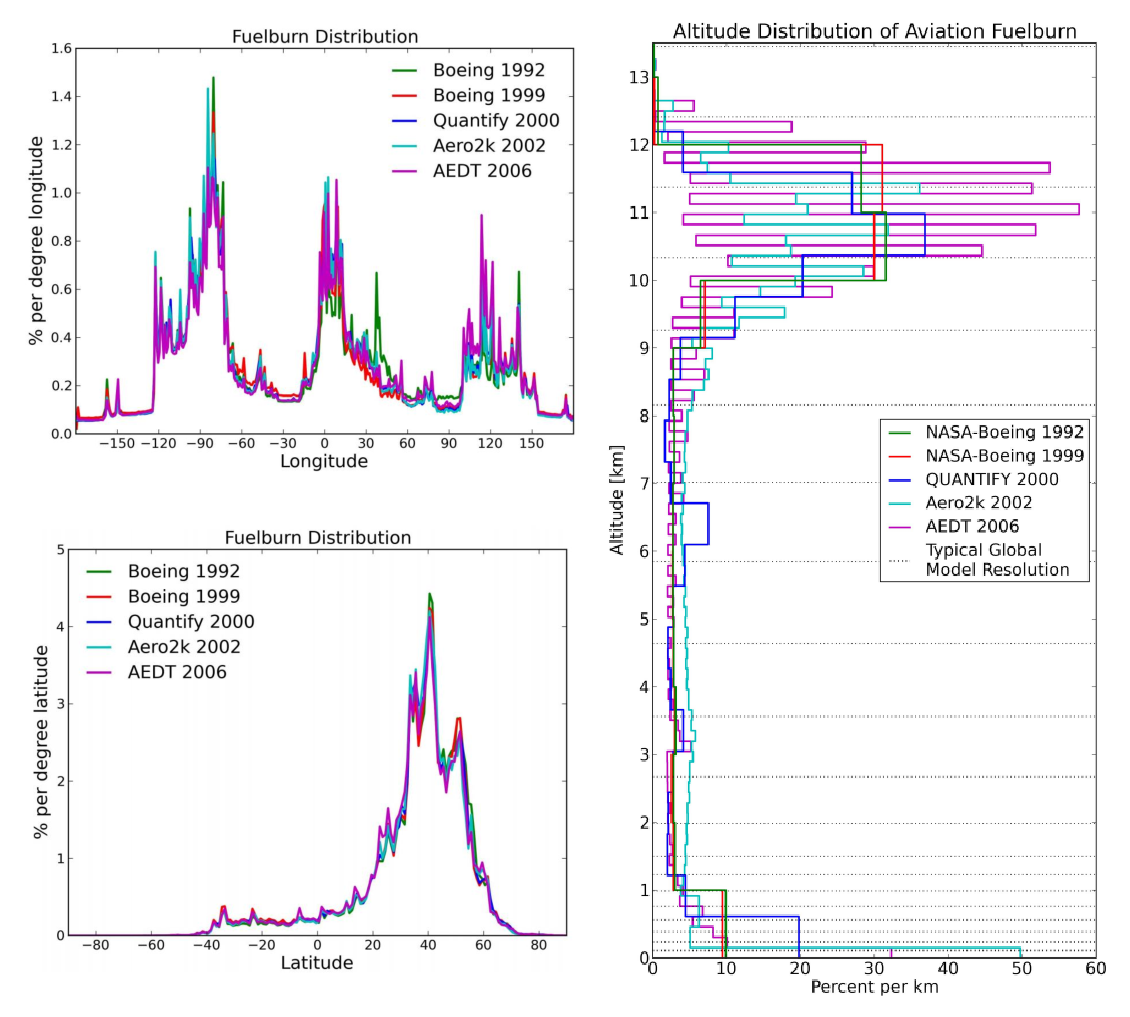
\includegraphics[width=0.8\linewidth]{FB_dist_spatial.pdf}
  \caption{Spatial (latitude, longitude and altitude) distribution of global aviation fuel burn from a range of aircraft emissions datasets \cite{Olsen2013}.}
  \label{FB_dist_spatial}
\end{figure}

The climate sensitivity of the atmosphere is highly variable depending on the exact latitude, longitude and altitude combination, because of the spatially varying chemical and meteorological state of the atmosphere (e.g. \cite{Houghton2001, Inness2013, Emmons2000}). Accurate accounting of spatial distribution patterns of air traffic is therefore very important in the estimation of aviation climate impact. Figure \ref{FB_dist_spatial} shows the spatial distribution of fuel burn across the range of datasets in the longitudinal, latitudinal and vertical directions. The longitudinal distribution shows three emissions peaks around the densely-populated regions of the US, Europe and East Asia, with the largest situated above the North American land mass. It is evident in the latitudinal distribution, that the Northern Hemisphere dominates, with a strong peak in the northern mid-latitudes that appears due to high volumes of air traffic above the US and Europe, as well as along the connecting region of airspace, the North Atlantic flight corridor (NAFC). Contrarily, there are almost no emissions present in southern latitudes below 40\textdegree~S, with the region between 40\textdegree~S and the equator constituting only a small percentage. The altitudinal distribution on the other hand, experiences emissions peaks around both the low altitude LTO area and the high-altitude cruising regions between 9 and 13~km, with relatively low emission intensities at mid-altitudes. Furthermore, the peak around cruising altitude is discretised into peaks every other flight level, due to the vertical separation constraints and the allocation of aircraft to specific flight levels, thus owing to further increases in emissions intensities at these altitudes.

%Similarly, Wasiuk et al.\ (2016) \cite{Wasiuk2016} derived global \ce{NO_x} emissions totals for 2005 to 2011 by coupling an aircraft emissions modelling framework with an air traffic dataset for this period. Aircraft performance was modelled for each flight in the dataset using the BADA3 method \cite{Nuic2010} and the emissions were calculated using the BFFM2 \cite{DuBois2006}. Figure \ref{Wasiuk_fig} portrays the spatial distribution of \ce{NO_x} emissions on a latitude-longitude map averaged over the six year period. For both altitude bands, main areas of aviation activity such as flights over mainland and popular flight corridors are highlighted. The outcome of this analysis suggests similar findings to that of Olsen et al. for both the latitude and longitude plots in figure \ref{FB_dist_spatial}. In the longitude plots in figure \ref{Wasiuk_fig}, the three main areas of activity remain prominent; mainland US, Europe and East Asia, along with the much more distinguishable flight corridors that connect these regions. In the latitude plots, the Northern Hemispheric skew is also present, with most air traffic remaining within 20 to 60\textdegree N and a peak occurring around 40\textdegree N.

%\begin{figure}[H]
%  \centering
%  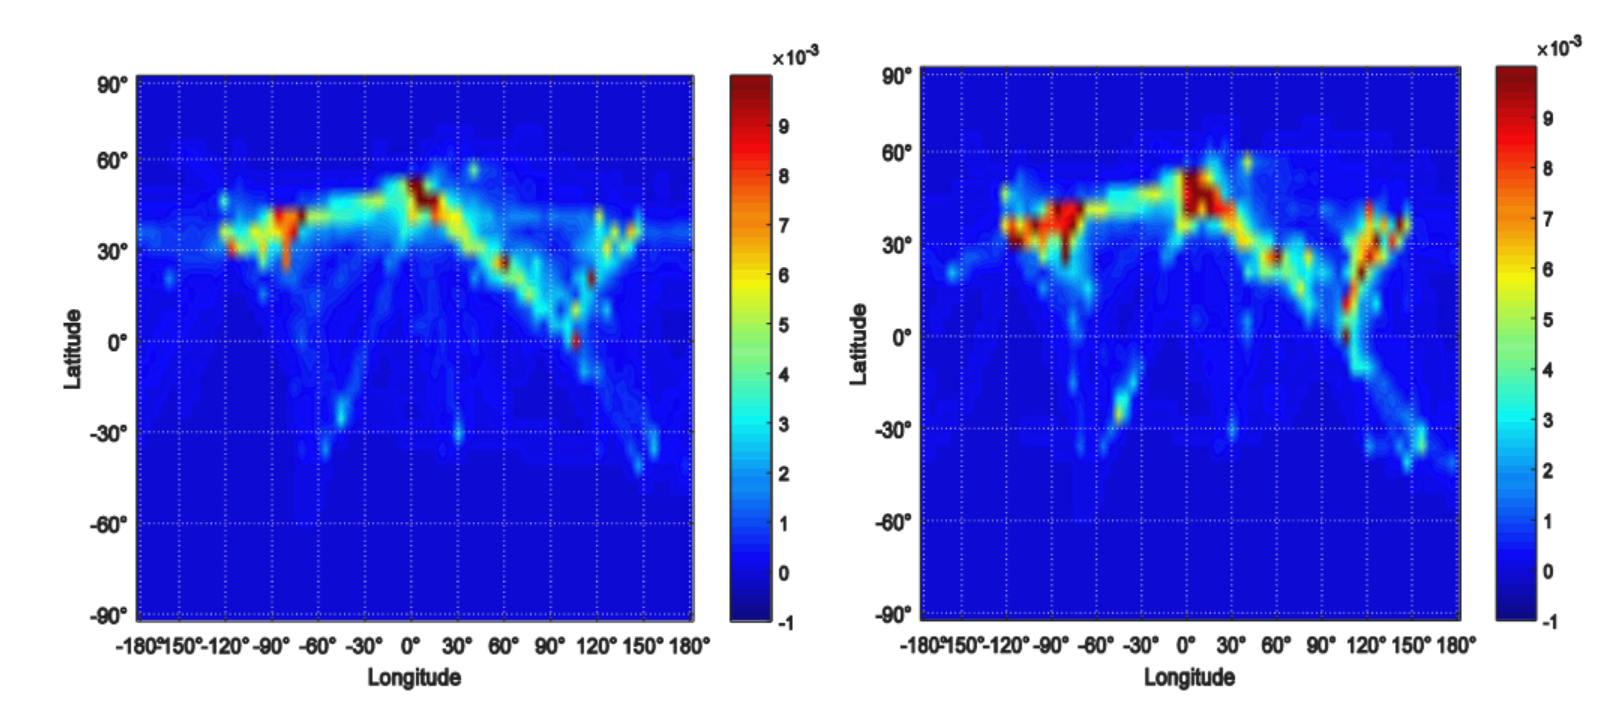
\includegraphics[width=\linewidth]{Wasiuk_fig.png}
%  \caption{}
%  \label{Wasiuk_fig}
%\end{figure}

The presence of diurnal and seasonal variations in key chemical and meteorogical parameters throughout the atmosphere has been widely investigated in the literature (e.g. \cite{Schanz2021}). The diurnal and seasonal variation in aviation fuel burn from Olsen et al.\ (2013) \cite{Olsen2013} is displayed in figure \ref{FB_dist_temporal}. The temporal fluctuations in both the state of the atmosphere and the distribution of fuel burn and emissions allude to the fact that the climate sensitivity to aircraft emissions is always changing, and therefore these parameters must be under constant observation to ensure accurate determination of global climate effects from aviation. The diurnal cycle of global aviation fuel burn, as seen on the left hand side of figure \ref{FB_dist_temporal} displays a peak at around 15:00~UTC, which decreases through the night until around 09:00~UTC where total fuel burn begins to increase again. With regards to seasonal variation, there is significant variance between emissions datasets, however in general, all display a wintertime minimum between December and January, and a summertime maximum between June and September.

\begin{figure}[H]
  \centering
  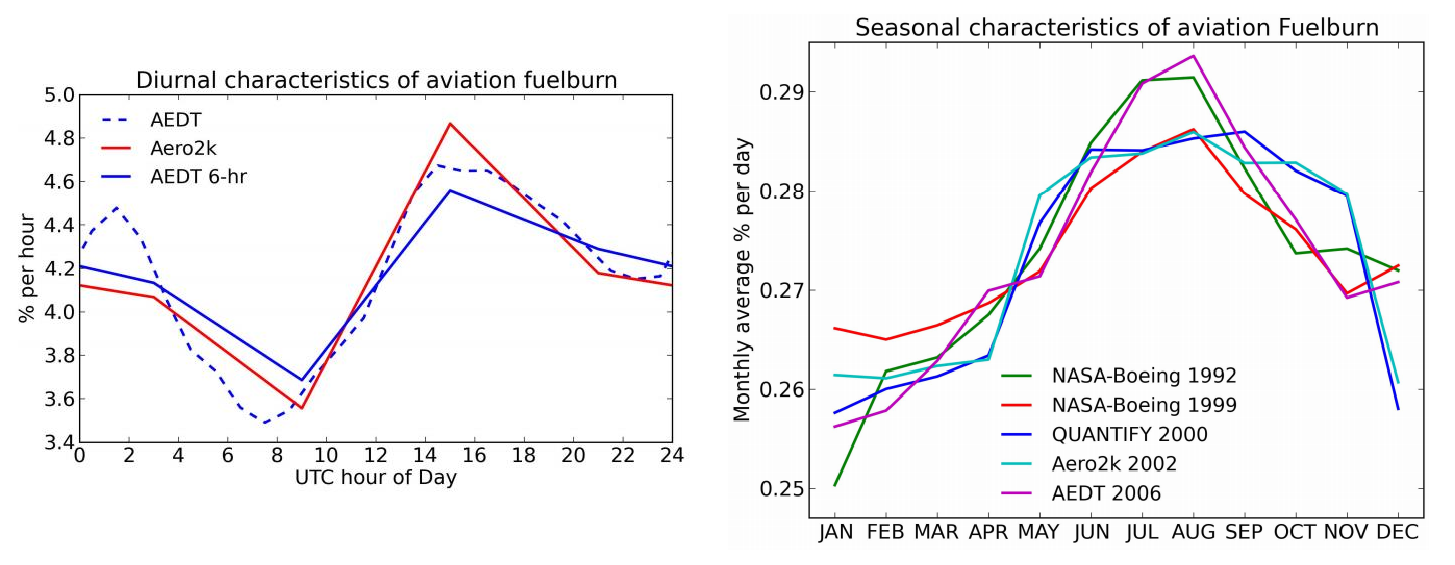
\includegraphics[width=0.8\linewidth]{FB_dist_temporal.pdf}
  \caption{Temporal (diurnal and seasonal) distribution of global aviation fuel burn expressed as percentage from a range of aircraft emissions datasets \cite{Olsen2013}.}
  \label{FB_dist_temporal}
\end{figure}

\subsection{Local air traffic and emissions distribution}
Due to the fixed-route nature of airspace, aircraft tend to fly along common airways or flight corridors, and pass common waypoints along their journey, leading to exceptionally high flux densities of aircraft through these regions at peak times. This has implications on the nonlinear chemical and physical effects occurring at the plume scale, due to the intersection of aircraft plumes and the elevated exhaust gas concentrations entrained within them. A prime example of a high-density airspace region is the NAFC, made up of a series of tracks that aircraft traversing the North Atlantic must follow, updated daily to allow for convective weather avoidance, tracking of the North Atlantic Jet Stream and favourable tailwinds to maximise efficiency \cite{NOTAMS}. The annually-averaged number of aircraft traversing the NAFC per day has increased from 800 in 1997 \cite{Karcher1998} to around 2,500 in recent years \cite{NATS_NAFC}, owing to the tripling of passenger demand since then \cite{World_databank}. With North Atlantic air traffic being confined to a limited number of tracks (usually three or four), it can be assumed that aircraft separation distances and airspace capacities are pushed to their limit on a regular basis along this and other popular flight corridors around the world.

%Schlager figure here

Previous experimental work on air traffic emissions in the NAFC was carried out in the late 1990's, through campaigns such as the Pollution from Aircraft Emissions in the North Atlantic Flight Corridor (POLINAT) and Subsonic Assessment Ozone and Nitrogen Oxide Experiment (SONEX) \cite{Schumann2000}. At least 20 follow up papers were published following these campaigns, in which POLINAT/SONEX data are utilised to provide insight on a number of major scientific issues \cite{Thompson2000}. A noteworthy publication with regards to localised emissions impacts is Schlager et al.\ (1997) \cite{Schlager1997}, which carries out an in-situ investigation of air traffic emissions signatures (nitrogen oxides (\ce{NO_x}), sulphur dioxide (\ce{SO_2}) and cloud condensation nuclei (CCN)) in the NAFC using experimental data from a POLINAT research flight. The research aircraft flew perpendicular to the major eastbound corridor tracks and took measurements of various chemical concentration fields and meteorological parameters throughout. The results show that the superposition of aircraft exhaust plumes led to peak concentrations of \ce{NO_x}, \ce{SO_2} and CCN above background levels by factors of 30, 5 and 3, respectively. This is because plume dispersion timescales greatly exceed the daily frequency with which aircraft emissions are input into the flight corridor, resulting in an inhomogeneous concentration field with narrow and sharp peaks over a relatively low and smooth background level \cite{Schumann2000}.

\begin{figure}[H]
  \centering
  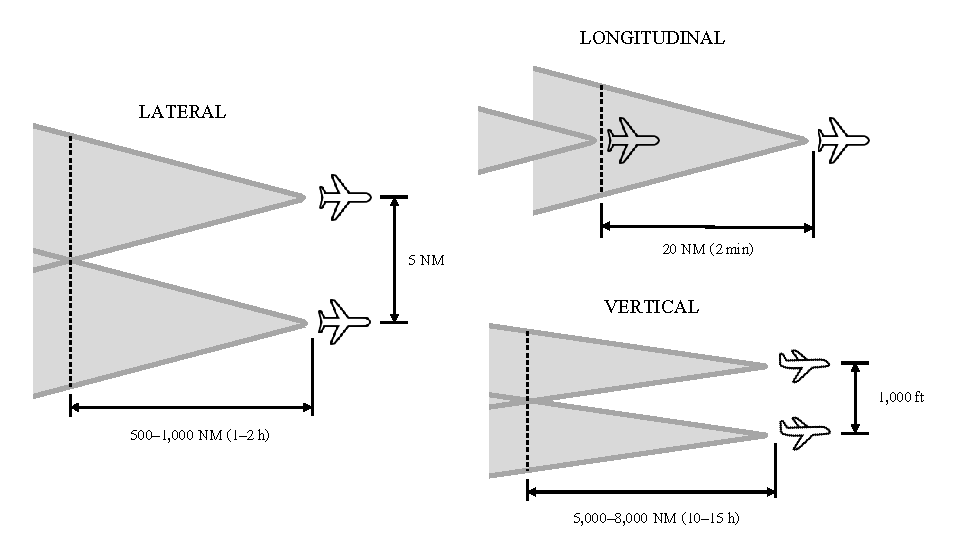
\includegraphics[width=0.9\linewidth]{cap_example.pdf}
  \caption{Lateral, longitudinal and vertical maximum plume overlap scenarios, based on nominal separation minima \cite{ICAOPANSDoc44442016}}
  \label{cap_example} 
\end{figure}

In the observation of plume-scale climate effects in high-density airspace regions, aircraft separation minima determine the minimum possible distance between aircraft and hence the maximum possible overlap between aircraft exhaust plumes. The degree of plume overlap influences the magnitude of emissions saturation, further accentuating nonlinear plume-scale climate processes that occur, as elaborated on in section \ref{Saturation}. Using plume dimension estimates from Kraabol et al.\ (2000a) \cite{Kraabol2000a}, maximum plume overlap scenarios can be inferred. Figure \ref{cap_example} displays the lateral, longitudinal and vertical maximum overlap scenarios for aircraft cruising at 550~kt. The longitudinal separation scenario proves to be the most effective formation for superimposing aircraft plumes, with the intersection time simply equalling the time taken to travel the separation distance between the two aircraft. For lateral and vertical superposition, the intersection time is much longer, as it is determined by the plume expansion rate in that particular direction, up until the midpoint between the two aircraft is reached. For lateral plume overlap to occur, the plumes must expand horizontally to a radius of 2.5~NM (15,190~ft), whereas for vertical, the distance is a mere 500~ft. Despite the drastic reduction in distance, the vertical plume overlap takes about an order of magnitude longer than lateral, because vertical plume expansion is substantially suppressed in comparison due to stable atmospheric stratification counteracting vertical motion \cite{Schumann1995}. In reality, air traffic flows are much more complex and the controlled and orderly formations shown in figure \ref{cap_example} are unlikely to occur naturally. However, the premise still holds that plume overlap occurs most frequently in congested flight corridors such as the NAFC, when aircraft travel along similar tracks and the vertical displacement between aircraft is minimal. 

The importance of safety, order and efficiency in the air traffic management process and the characteristics of global and local air traffic flows have been discussed. As the following section will explore, the atmospheric response to aviation emissions is highly sensitive to time and location, because the instantaneous state of the atmosphere (i.e. the chemical composition and meteorological situation at that particular time and position) determines the production, loss and radiative response of key chemical species that induce climatic effects \cite{Jacobson2005}. With insight into how air traffic and emissions are dispersed locally and distributed globally, the contribution of aircraft emissions to climate change can be more rigorously evaluated.

 %on a global and local scale, through evaluation of the climate forcing mechanisms that result from emissions and analysis of their relative global warming contributions. 

%Further to this, the nonlinear chemistry and microphysics within the exhaust plume is covered in great detail. % < Probably needs some work.

%Based on 1997 market analysis, it was found that the annually-averaged number of aircraft traversing the NAFC per day is 800 \cite{Karcher_1998}, around FL350 with a cross sectional area of 2000km$^2$. This corresponds to one aircraft passing a fixed point along the corridor every 100s or so. Accounting for the fact that air traffic is confined to a small number of tracks (usually 3 or 4) within the corridor, and that air traffic passenger demand has tripled since then, it can be safely assumed that aircraft separation distances are close to minimum and airspace capacities are pushed to their limit on a regular basis. \cite{Schlager_1997} carries out an in-situ investigation of air traffic emissions signatures in the NAFC, and 

%Using a standard plume distribution and assuming aircraft are separated at a minimum distance in all three directions, worst-case plume overlap scenarios can be deduced. which serve as a theoretical foundation for studies observing the effects associated with multiple overlapping plumes.






\section{The global climate impact of aviation}
\label{climate}
Aircraft emissions induce climate effects by perturbing the flux of inbound shortwave (SW) solar radiation and outbound longwave (LW) terrestrial radiation emitted from the Earth's surface through absorption and scattering processes that give rise to warming or cooling of the atmosphere \cite{Myhre2013}. Climate metrics such as radiative forcing can be used to measure the climate contribution of each individual emission species, enabling the determination of the net global warming effect from aviation. This section explores the potential global impact of aviation deduced from measurement and modelling of atmospheric processes.

%Accurate quantification of aviation's climate impact requires sufficient modelling of plume-scale effects that are neglected in global models. The accumulation of aircraft emissions in high-density flight regions can lead to saturation effects which affect aviation's net warming effect. This section elaborates on the literature associated with these research areas, to help the reader conceptualise why the atmospheric response to aircraft emissions is dependent on background ambient conditions, and hence why it is also influenced by the presence of other aircraft exhaust plumes in close vicinity.

\subsection{Aircraft emissions in the Upper Troposphere and Lower Stratosphere}
As figure \ref{FB_dist_spatial} suggests, the vast majority (\textasciitilde60\%) of aviation fuel burn and hence aviation emissions, occur at cruise altitudes, between 9 and 13~km vertically. The region of the atmosphere encompassing this volume of airspace is known as the Upper Troposphere and Lower Stratosphere (UTLS), with bounds of $\pm$5~km above and below the conventional tropopause \cite{Gettelman2011}. Around 20--40\% of total aircraft emissions are released in the LS \cite{IPCC1999, Hoinka1993} and the rest are released in the troposphere, extending from the surface at take-off to the UT at aircraft cruise altitudes. The greenhouse effect due to the release of chemically-active substances in the UTLS is considerably greater than that of emissions at the surface. This is because the climate in the UTLS is more sensitive due to increased residence times of pollutants, lower background concentrations (meaning emissions have a greater influence on the atmospheric chemistry), lower temperatures which drive reversible reactions in an unfavourable direction, and finally, a higher radiative efficiency which gives rise to more efficient photochemistry \cite{Schumann1997}. Johnson et al.\ (1992) \cite{Johnson1992} further validates this claim, with model results concluding that \ce{NO_x} emissions constitute a 30 times greater climate impact in the UT compared to equivalent surface emissions, due to the absence of direct deposition and slower conversion to stable reservoir species at aircraft cruising altitudes.

Despite such a large proportion of air traffic emissions being released into the LS region, it is thought that the perturbation to the chemical and radiative state of the stratosphere is negligible, as the vast majority of species emitted into the stratosphere are transported downwards into tropospheric regions, where they interact with the atmosphere there \cite{Lee2010, Grewe2002, Forster2003}. Henceforth, this review will primarily focus on the tropospheric response to aircraft emissions, except for water vapour, where the stratospheric climate response becomes particularly noteworthy.

\subsection{Radiative forcing of aircraft emissions}
High altitude emissions from aviation impact the climate through a variety of climate forcing pathways. Some greenhouse gases such as \ce{CO_2} and \ce{H_2O} are emitted directly, others are produced indirectly through chemical processing of aircraft emissions, such as the reaction of \ce{NO_x} with atmospheric trace species to catalyse ozone production and methane destruction. Water vapour and PM emissions are responsible for the formation of high ice clouds known as condensation trails (contrails), which often trap outbound LW radiation within the atmosphere more efficiently than they reflect inbound SW radiation. PM emissions also have the potential to induce a climate perturbation through direct radiative processes due to aerosols, which may warm or cool the climate depending on the particle's optical and microphysical properties \cite{Lee2010}. Diversity in the climate forcing pathways for each emission species means that the only reliable method of determining the severity of each climate contribution is to model the atmospheric response and determine the resulting impact on the radiative flux of the atmosphere \cite{Brasseur1998}.

The most common climate metric used to compare the magnitudes of climate impact from a range of emission species is radiative forcing (RF). RF is defined as the perturbation to the net energy balance of the Earth-atmosphere system due to natural or anthropogenic factors of climate change, measured in watts per square metre [\ce{Wm^{-2}}] \cite{Fuglestvedt2003}. A positive RF means that the climate forcing mechanism is inducing a warming effect and vice versa. Lee et al.\ (2021) \cite{Lee2021} presents an updated analysis of the global effective radiative forcing (ERF) contributions for aviation-induced climate change. ERF is a newly proposed climate modelling framework that builds upon the RF concept by removing rapid atmospheric adjustments that bear no relation to the long-term surface temperature response that occurs over decadal timescales \cite{Myhre2013}. ERF serves as a more suitable equivalency metric to compare the global warming response of heterogeneously distributed short-lived climate forcers and uniformly distributed long-lived climate forcers. Figure \ref{Lee2021} displays the ERF and RF contributions for each of the key aviation-induced climate forcers.

\begin{figure}[H]
  \centering
  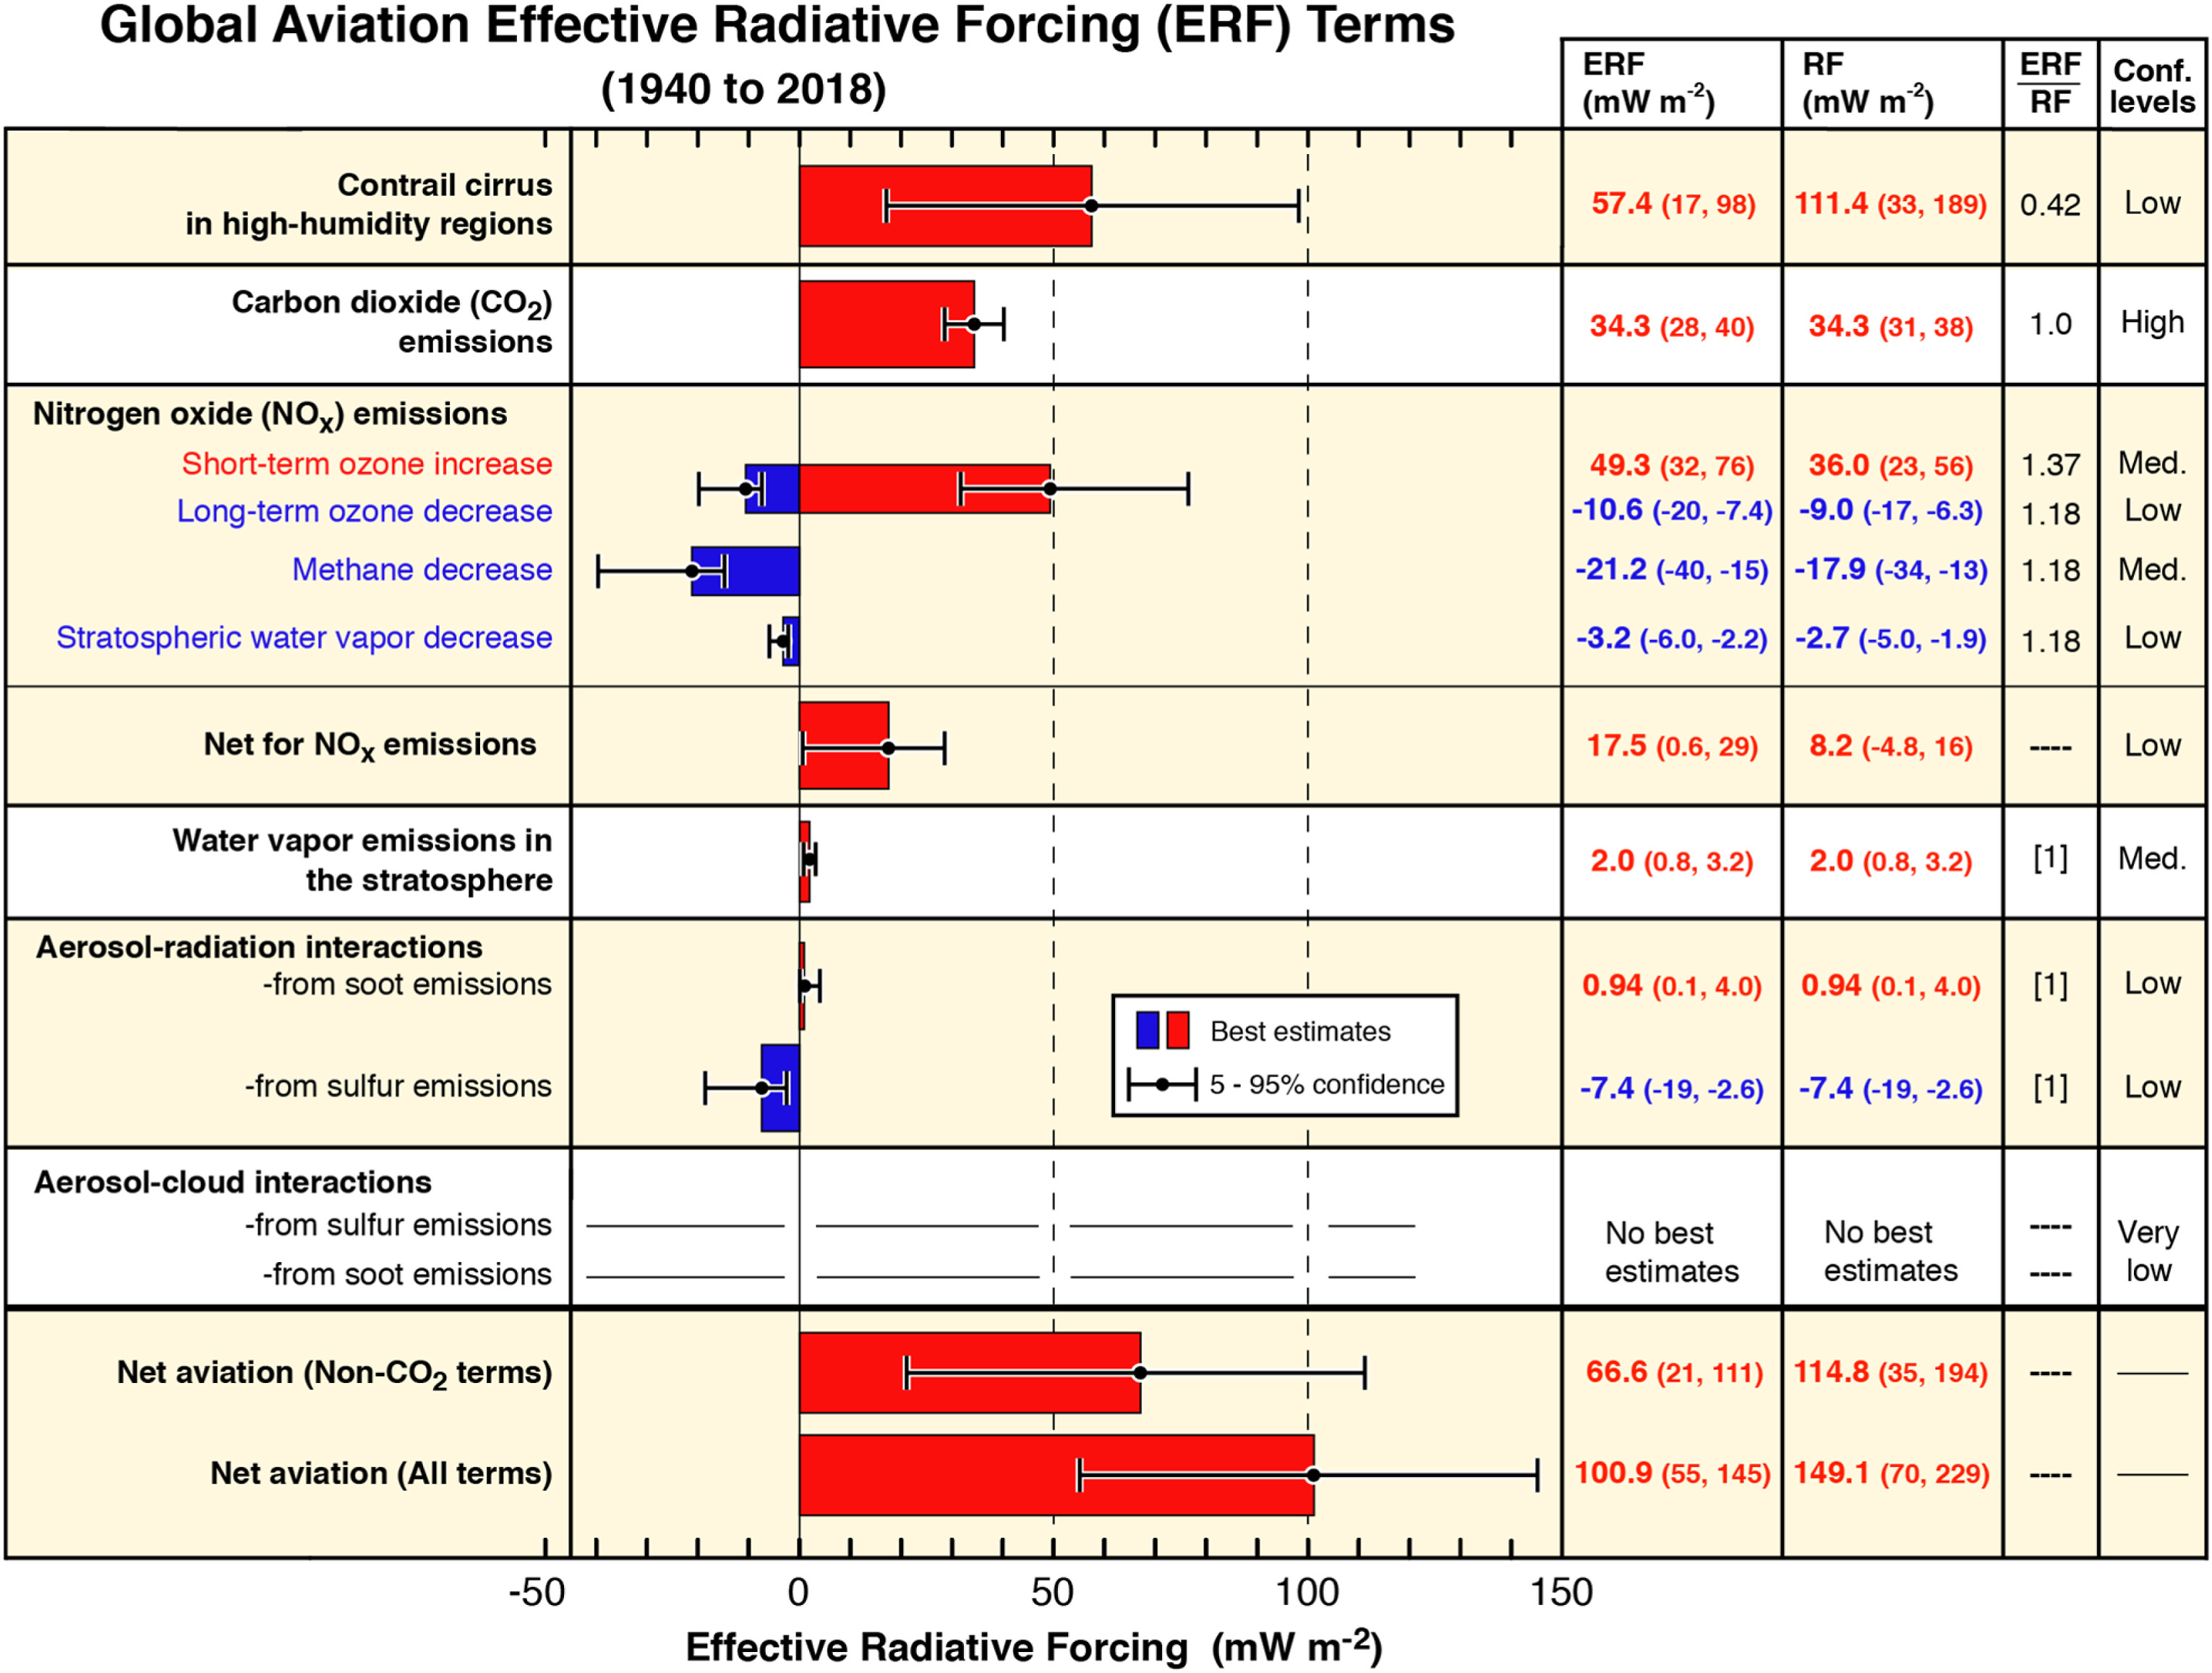
\includegraphics[width=0.9\linewidth]{Lee2021.jpg}
  \caption{Radiative forcing contributions from global aviation between 2000 and 2018 \cite{Lee2021}. Error bars represent 5--95\% confidence interval, with corresponding RF and ERF values shown in parentheses.}
  \label{Lee2021}
\end{figure}

\subsubsection{\ce{CO_2}}
The climatic effects of aviation \ce{CO_2} emissions are direct and well understood, with the thermal absorption of outbound LW radiation leading to warming through the planetary greenhouse effect \cite{Schneider1989}. Carbon dioxide from aircraft constitutes the second largest ERF term in figure \ref{Lee2021} at 34.3~\ce{mWm^{-2}}, and the thermodynamic and photochemical stability of \ce{CO_2} means it has a relatively long atmospheric lifetime, on the order of 100 to 1,000 years \cite{Archer2008}. This means that carbon emissions from aircraft simply serve to increase its atmospheric concentration, leading to the eventual distribution over global spatial scales. The ubiquitous and intuitive nature of \ce{CO_2}-related warming deems it a suitable benchmark to compare warming from non-\ce{CO_2} climate forcers against. The assumption of instantaneous dilution in global models is sufficient for modelling the climate impact due to carbon dioxide, as it exists over vast spatial and temporal scales, meaning the climatic effects occurring on plume time scales are negligible compared with the impact induced over its entire lifetime \cite{Paoli2011}.

\subsubsection{Contrail cirrus}
When emissions of water vapour and PM are released into the aircraft exhaust plume in the cold and moist condition of the UTLS, the water vapour condenses around the particulates due to the high relative humidity (RH), then freezes due to the low external temperatures, permitting the formation of ice crystals. The accumulation of ice crystals in the aircraft wake gives rise to the generation of a condensation trail, also known as a contrail. The evolution of contrails, i.e. how they grow, disperse and persist with time, is largely determined by the ambient conditions of the surrounding atmosphere, with lower temperatures and higher humidities generally leading to more persistent and damaging contrails \cite{Schumann2005}. The formation and persistence of contrails can be predicted purely from the thermodynamic assumption that, as the hot and moist exhaust mixes with the colder and drier ambient air, a contrail will form if the plume exceeds water-saturation at any point and the temperature is low enough for ice nucleation to occur. A contrail will persist in the atmosphere if it mixes with air that is supersaturated with respect to ice, i.e. an ice-supersaturated region (ISSR), growing with time due to deposition of surrounding water vapour onto existing ice crystals \cite{Karcher2018, Schumann2005}. Persistent contrails can sometimes transition to contrail cirrus, either building onto existing cirrus clouds or forming new ones, spreading over vast swathes of the atmosphere \cite{Minnis1998} and inducing significant radiative effects. ISSRs occur frequently at aircraft cruising altitudes and often span hundreds of kilometres horizontally, however only reach depths of 100 to 1,000~m \cite{Spichtinger2016, Dickson2010}. Their shallow nature means that aircraft can avoid them by changing flight level by $\pm$2000~ft to minimise persistent contrail generation for a minor additional fuel penalty \cite{Schumann2011}.

The optical characteristics of contrail ice crystals often exhibit significant levels of opacity, tending to absorb outbound terrestrial radiation more efficiently than they reflect inbound solar radiation. This induces a globally averaged ERF of 57.4~\ce{mWm^{-2}}, meaning, despite their relatively short lifetime in comparison, the current contrail effect contributes more to climate change than the accumulation of aviation carbon, since the dawn of aviation \cite{Burkhardt2011}. Contrail evolution, i.e. how they grow, disperse and persist with time, is largely determined by the ambient conditions of the surrounding atmosphere, with lower temperatures and higher humidities generally leading to a more persistent and damaging contrails \cite{Schumann2005}. The formation and persistence of contrails can be predicted purely from the thermodynamic assumption that, as the hot and moist exhaust mixes with the colder and drier ambient air, a contrail will form if the plume exceeds water-saturation at any point and the temperature is low enough for ice nucleation to occur. A contrail will persist in the atmosphere if it mixes with air that is supersaturated with respect to ice, i.e. an ice-supersaturated region (ISSR) \cite{Karcher2018}. 

%The thermodynamic constraints for contrail formation and persistence were first theorised by Schmidt (1941) \cite{Schmidt1941} and Appleman (1953) \cite{Appleman1953}, based on prior empirical observations \cite{Schumann1997b}, that led to the promulgation of the so-called ``Schmidt-Appleman (SA) criterion". The SA criterion shows that the contrail formation threshold is purely dependent on ambient pressure, relative humidity, and the ratio of water and heat released into the exhaust plume, assuming isobaric mixing between exhaust emission and full dilution into the ambient atmosphere \cite{Schumann1996}. See Tait (2020) \cite{Tait2020} for a detailed description of how the SA criterion can be illustrated on a plot of water vapour partial pressure against temperature. Contrails which surpass water saturation, but do not settle in ice-supersaturated air are generally assumed to be short-lived, as the ice sublimates and deposits into the surrounding atmosphere. However, contrails released into ISSRs, where the ambient humidity is higher than the saturation humidity over ice surfaces, instead grow with time because the ice particles experience deposition of surrounding water vapour molecules \cite{Schumann2005}. Persistent contrails can sometimes transition to contrail cirrus, either building onto existing cirrus clouds or forming new ones, spreading over vast swathes of the atmosphere \cite{Minnis1998} and inducing significant radiative effects. ISSRs occur frequently at aircraft cruising altitudes and often span hundreds of kilometres horizontally, however only reach depths of 100 to 1,000~m \cite{Spichtinger2016, Dickson2010}. Their shallow nature means that aircraft can avoid them by changing flight level by $\pm$2000~ft to minimise persistent contrail generation for a minor additional fuel penalty \cite{Schumann2011}.

%Contrails released into ice-subsaturated air will be short-lived, as the ice particles sublimate in ambient air within a matter of seconds to minutes, meaning the radiative impact is negligible \cite{}. However, contrails released into ISSRs, where the ambient humidity is higher than the saturation humidity over ice surfaces, instead grow with time because the ice particles experience deposition of surrounding water vapour molecules \cite{Schumann2005}. This allows the contrails to persist in the atmosphere for hours and potentially transition into cirrus clouds with vast areal coverage \cite{Minnis1998, }. Persistent contrails and contrail cirrus induce a significant climate impact due to the 

Contrails exhibit radiative forcing through the obstruction of both SW and LW radiative fluxes, with areal coverage and optical depth (opacity) being the key drivers of contrail climate impact \cite{Schumann2017}. A contrail's emissivity (ability to absorb and re-emit infrared LW radiation back towards Earth) and reflectance (ability to reflect inbound SW radiation back out to space due to scattering at visible wavelengths) is a function of contrail optical depth and ice particle microphysics. Contrails and other high ice clouds often warm the climate, as their thin optical depth means partial transparency to solar radiation, whilst their high ice density traps infrared radiation within the atmosphere effectively \cite{Karcher2018}. Contrail RF also displays a distinct diurnal trend; at night, contrails always induce a warming effect, as there is no SW scattering to counteract the LW absorption. During the day, contrails display a reduced net warming effect and perhaps even a net cooling effect, depending on the amount of solar radiation that is redirected back out to space \cite{Newinger2012}. The SA criterion can be used to predict formation and persistence of contrails, however accurate quantification of contrail RF requires sufficiently detailed microphysical modelling, to deduce key information on the underlying formation mechanisms and physical and optical properties the contrail exhibits throughout its evolution \cite{Karcher2015}. See section \ref{Microphysics} for elaboration on the microphysical processes that determine a contrail's radiative characteristics, and how these processes can be parametrised for modelling purposes.

%Contrail EF concept, similar to other climate metrics, takes into account temporal dimension.

\subsubsection{Net-\ce{NO_x}}
Nitrogen oxides (NO and \ce{NO_2}) released from aircraft are not radiatively active and therefore do not induce an immediate climate impact at the point of emission. Their chemical instability does however mean that they exhibit a number of indirect RF effects, due to the chemical reactions that occur following dilution into the ambient atmosphere. The chemical interactions between \ce{NO_x} and trace species in the background atmosphere at aircraft cruising altitudes are highly non-linear and thus, the net-\ce{NO_x} RF contribution is dependent on the instantaneous atmospheric state (time of day and year, latitude, background chemical composition, meteorological situation) \cite{Fritz2020, Kraabol2000b}. 

Emissions of \ce{NO_x} in the troposphere initially leads to the short term local increase in ozone production efficiency (\ce{O_3}) on the time scale of weeks to months. In addition, elevated \ce{NO_x} and \ce{O_3} levels lead to increased hydroxyl radical (OH) production, which in turn, leads to the long term global destruction of ambient methane (\ce{CH_4}) over the time scale of decades \cite{Stevenson2004, Wild2001, Myhre2011}. The short term increase in \ce{O_3} generates a strong positive ERF of 49.3~\ce{mWm^{-2}}, whereas the long term \ce{CH_4} depletion causes a lesser negative ERF of -21.2~\ce{mWm^{-2}} in comparison, however there are a number of secondary negative radiative effects arising from methane depletion that must also be accounted for. This is the reduction in stratospheric water vapour (15\% \ce{CH_4} RF magnitude) and a decrease in long-term background ozone in the troposphere (45\%~\ce{CH_4} RF magnitude), resulting from reduced background \ce{CH_4} concentrations \cite{Holmes2011, Myhre2007}. Despite the long-term negative cooling effects, the short term warming from \ce{O_3} dominates, leading to a largely positive net ERF of 17.5~\ce{mWm^{-2}} overall, as seen from figure \ref{Lee2021}. Section \ref{Gas-phase_photochem} explores the nonlinear \ce{NO_x}-\ce{O_3} relationship further through explanation of the gas-phase photochemical processes that begin in the aircraft plume and are eventually distributed to regional and global scales. 

\subsubsection{Water vapour}
The direct radiative effects induced by aviation water vapour emissions in the troposphere are insignificant, because the influence on background concentrations is negligible when compared with the natural fluxes of the Earth's hydrological cycle \cite{IPCC1999}. Any tropospheric water vapour emissions tend to get lost through deposition, due to high humidity and precipitation in this region, leading to a lifetime of around 9 days. On the contrary, water vapour that is emitted into the stratosphere (without getting transported downwards into the UT) can induce a considerable effect on the surrounding environment, due to extreme dryness at these altitudes \cite{Jensen1996}. This is because increases in stratospheric water vapour (SWV) concentrations impact the climate directly through the greenhouse effect, as well as through influences on the gas-phase and aerosol chemical composition, leading to depletion of ozone and altering the formation and growth of polar stratospheric clouds \cite{Stenke2005}. The combined impact of the direct greenhouse effect and indirect impacts on ozone and polar stratospheric clouds due to increased SWV leads to an overall ERF of 2.0~\ce{mWm^{-2}}.

As proposed in Lee et al.\ (2010) \cite{Lee2010}, the relatively small climate perturbation due to aviation-induced SWV has the potential to increase drastically as future flight concepts begin to take shape. This includes the environmental implications associated with the potential replacement of the current subsonic aircraft fleet with a supersonic high-speed civil transport (HSCT) fleet, that primarily operates in the stratosphere (e.g. \cite{MiakeLye1993, Danilin1994, Grooss1998, Kawa1999}). Furthermore, the prospect of transitioning the entire subsonic kerosene-based commercial fleet to a hypothetical fleet of cryoplanes (hydrogen-powered aircraft with zero carbon emissions) would increase aviation \ce{H_2O} emissions by a factor of \textasciitilde2.5 \cite{Gauss2003}. In the high-humidity conditions of the UT, this brings about the potential for large increases in contrail production, whereas in the LS, this would induce significant perturbations to SWV concentrations.

%However, the present air traffic increases background humidity by less than 1.5\% for regions most frequently used by aircraft. Increased water vapour in the stratosphere also affects the rate of chemical ozone loss, e.g., by increasing the incidence of polar stratospheric clouds.

\subsubsection{Aerosol effects}
Aviation aerosol particles, either emitted directly post combustion, or formed in the wake of the aircraft, can perturb the energy balance of the atmosphere directly, as well as indirectly through the formation of contrail ice particles and heterogeneous chemical processing. The direct aerosol effect is primarily produced by the key non-volatile and volatile PM emissions: soot and sulphate aerosols.

Soot exhibits a direct radiative forcing as it has the strongest absorption of light at visible wavelengths per unit mass, more than any other abundant substance in the atmosphere, thus contributing to global heating through absorption of inbound solar radiation and light rebounded off reflective surfaces such as snow and ice \cite{Bond2013}. The resultant heating of the atmosphere and reduction of sunlight can affect the hydrological cycle and large-scale circulation patterns, having potentially larger implications on the climate than previously thought. Despite its ability to strongly absorb sunlight, aircraft soot is responsible for only a few percent of total atmospheric black carbon, meaning the aerosol-radiation interaction brought about by aviation soot only constitutes a minor ERF of 0.94~\ce{mWm^{-2}}.

Sulphur dioxide (\ce{SO_2}) is formed when sulphur, which is present in hydrocarbon jet fuels, oxidizes during the combustion process \cite{Brown1996}. \ce{SO_2} that is emitted from the aircraft exhaust can be oxidised to form gaseous sulphuric acid (\ce{H_2SO_4}), which may condense on existing particles or contribute to new particle formation in low-condensation environments, resulting in sulphate aerosol formation. Sulphate aerosol is mainly composed of sulphuric acid and corresponding salts such as ammonium sulphate. The optical properties of sulphate mean that it tends to scatter inbound sunlight, thus leading to a net negative (cooling) of 7.4~\ce{mWm^{-2}}, that sways the net direct climate impact of aviation aerosols towards cooling. 

It is relatively well established that aviation-induced aerosols have a direct impact through radiative interactions, as discussed in this section, as well as indirectly through activation of water vapour on PM emissions through contrail formation. There are however, potentially large indirect consequences of aerosol particles interacting with cloud droplets and ambient ice particles nucleation on the aerosol surface. These effects are left without ERF estimates in figure \ref{Lee2021}, as there is great uncertainty around the accuracy of cloud process modelling and the ability to distinguish aircraft-induced clouds and natural clouds \cite{Penner2018}.

\subsection{Global climate modelling}
\label{Climate_modelling}
Quantifying aviation's global climate impact requires the use of computational climate models to predict the atmospheric response to the emission species released by aircraft. Climate models simulate the climate system through mathematical representation of established physical laws (e.g. conservation of mass, energy and momentum) and a plentiful supply of empirical data obtained through real world observation and measurement of physical and chemical quantities (e.g. chemical concentrations, meteorological parameters) \cite{Randall2007}. Gridded aircraft emissions inventories are used as input to climate models \cite{Olsen2013, Wilkerson2010}, in which emissions are homogeneously distributed throughout the entire grid cell that they are released into (i.e. the ID approach). The chemistry, physics and dynamics of the atmosphere are captured in the model, along with the perturbation to the atmospheric state due to emissions, providing an output of the spatial and temporal distributions of chemical species. Radiative transfer schemes can then be used to quantify the climate response to the perturbed chemical composition through instantaneous metrics such as RF and ERF. The variability in chemical and radiative properties of climate forcing species does however vary considerably with time. For example, \ce{CO_2} is distributed globally and affects the climate gradually over centuries, whereas contrails induce a severe yet short-lived, localised radiative impact \cite{Lee2021}. Therefore, metrics such as Global Warming Potential (GWP, GWP*) and Global Temperature Potential (GTP) have been developed to better account for the temporal variation of certain properties, providing a more well-rounded analysis of the climate contributions of aircraft emission species \cite{Fuglestvedt2003, Fuglestvedt2010, Cain2019}.

There are two main climate model distinctions for use in aviation climate modelling: general circulation models (GCMs) and chemistry-transport models (CTMs). GCMs are highly sophisticated, yet very complex, as they are what are known as ``online'' models, calculating chemical composition, temperature and transport circulation simultaneously and in real time. This is often computationally expensive and may require very long processing times to run, depending on the simulation. CTMs on the other hand are reduced order ``offline'' models, calculating chemical composition based on pre-determined GCM results or empirically observed temperature and transport circulation data \cite{IPCC1999}. Example usage of GCMs in aviation climate modelling include the European Centre HAmburg Model (ECHAM) \cite{Stevens2013} for analysis of future contrail cirrus radiative forcing \cite{Bock2019} and the Community Atmosphere Model version 5 (CAM5) \cite{Neale2004} to comprehensively represent aviation aerosol climate impact \cite{Gettelman2013}. CTMs appear much more frequently in the literature due to their versatility and computational efficiency. For example the UK Meteorological Office CTM STOCHEM \cite{Cooke2010} coupled with the Common Representative Intermediates (CRI) chemical mechanism \cite{Jenkin2008} is used for modelling the global impact of aviation \ce{NO_x} emissions on ozone production \cite{Wasiuk2014}, MOZART CTM \cite{Emmons2010} for use in investigating the trade-off between \ce{CO_2} and \ce{NO_x} emissions \cite{Freeman2017}, and another six CTMs are presented in \cite{IPCC1999} for aviation climate impact modelling purposes. Various model intercomparison studies provide an up-to-date, elaborate review of the models available for UT and LS (and thus aviation) climate modelling \cite{Roelofs2003}. 


%Climate models provide a realistic quantitative estimate of future climate change especially at the continental scale. In recent years, various climate models have been developed to improve understanding of climate processes and to perform more realistic time-dependent simulations of climate change. These models can incorporate physical processes in greater complexity such as coupling of climate system components and enhanced model resolution. The most sophisticated climate models are the General Circulation Models (GCMs) coupled with the chemistry scheme which can be used to study the potential anthropogenic influences on current and future climate \cite{Solomon2007}. However, the GCMs are very complex and computationally expensive, therefore may need very long processing time to run (depending on the climate perturbation) on a high-performance computer. To overcome this, simple climate models (SCMs) are used for estimating future climate impacts of aviation activity which are generally parameterized to reproduce the main characteristic responses of GCMs.

%SCMs are known as reduced complexity model, computationally inexpensive and widely used decision support tools for the policy makers. SCMs are used to evaluate climate impacts from a wide range of sources, from total anthropogenic emissions to sectoral emissions (e.g., aviation emissions). Model for the Assessment of Greenhouse Gas Induced Climate Change (MAGICC) is one of the SCMs which is not specific to aviation and can be used in different emissions scenarios to estimate time-dependent concentrations, radiative forcing, temperature response and sea-level rise from different perturbations \cite{Meinshausen2011}. Linear climate response model (LinClim) is a very effective SCM which has been customised specifically for aviation purposes. It implements a single impulse response function that is calibrated against more sophisticated parent GCM model. The global aircraft fuel emissions derived from emissions database and the calculated emissions indices are used to calculate historical, present day and future emissions trends of CO2, NOx, water vapour, sulphate and black carbon aerosols. LinClim calculates the climate impacts from non-CO2 species and contrails by scaling the emissions or distance travelled to an externally calculated base year radiative forcing. The carbon cycle in LinClim is based on the Maier-Reimer and Hasselmann (1987) \cite{} model and the CO2 RF is calculated using the function applied in IPCC AR468 \cite{Solomon2007}. The temperature response can be calculated by LinClim using radiative forcing and climate model parameters that are parameterized to LinClim’s parent GCM.

%The impact of the species released from aircraft on the atmosphere is non-linear. Thus, a non-linear climate-chemistry response model, AirClim \ce{Grewe2008} applicable to aviation industries is developed. This model comprises a linearisation of atmospheric processes from the emissions and productions of \ce{CO_2}, \ce{H_2O}, \ce{CH_4}, \ce{O_3} and contrails to radiative forcing, resulting in an estimate of surface temperature change.

%The FAA Aviation Environmental Portfolio Management Tool (APMT) uses impulse response models along with a simplified energy balance model to give aviation impacts for CO2, NOx on methane, NOx on ozone, sulphates, soot and contrails/contrails cirrus in terms of radiative forcing and global temperature change \cite{Marais2008}.





%\subsubsection{Instantaneous dispersion (ID)}
%Convention amongst the climate modelling community is to assume instantaneous dispersion (ID) of aircraft emissions into the dimensions of the latitude-longitude-altitude grid cell, whose size is determined by the model resolution. This ID assumption therefore neglects the presence of aircraft plume, and hence does not capture the aforementioned aircraft-induced dynamics which have a notable influence on the ensuing chemical and physical response of the atmosphere in real life \cite{}. Due to the lack of plume representation, ID modelling can be effected through simple analysis of the production and loss rates of an emission species, subject to instantaneous input of emissions concentrations at the time of release.


%Tropospheric chemistry is dominated by ozone (\ce{O_3}), a potent greenhouse gas which contributes to climate change and air quality issues. \ce{O_3} is an oxidant in its own right, reacting with reactive volatile organic compounds (VOCs, see later) but is the precursor to the OH radical, which is known as the chemical detergent of the lower atmosphere. The OH radical reacts with VOCs and allows them to be oxidised and removed from the atmosphere. Photolysis of ozone (absorption of sunlight in the UV region ~ 290-330 nm and the breaking of an O-O bond) starts the process of OH production, depicted by reaction (1), where hv denotes a photon of light;

%\begin{equation}
%	\ce{O_3 + hv -> O(^{1}D) + O_2}
%	\label{O3toO1D}
%\end{equation}
%
%Reaction \eqref{O3toO1D} makes a reactive oxygen atom \ce{O(^{1}D)}, that can either collide with N2 or O2 molecules (denoted as M) and be quenched to ground state \ce{O(^{3}P)} atoms in reaction \eqref{O1DtoO3P}
%
%\begin{equation}
%	\ce{O(^{1}D) + M -> O(^{3}P) + M}
%\label{O1DtoO3P}
%\end{equation}
%
%Or it can react with water to form HO radicals
%
%\begin{equation}
%	\ce{O(^{1}D) + H_2O -> OH + OH}
%\end{equation}
%
%OH radicals can then participate in chemical cycles that preserve levels but also remove pollutants, CO, in the following examples. First, under clean conditions (low \ce{NO_x} = NO and \ce{NO_2}) the following scheme (1) takes place:
%
%\begin{equation}
%	\ce{OH + CO -> H + CO_2}
%\end{equation}
%
%\begin{equation}
%	\ce{H + O_2 + M -> HO_2 + M}
%\end{equation}
%
%\begin{equation}
%	\ce{HO_2 + O_3 -> OH + 2O_2}
%\end{equation}
%
%Net reaction \ce{CO + O_3 -> CO_2 + O_2}
%
%Here, ozone is removed and CO is oxidised to form \ce{CO_2}, which, in a pre-industrial world, was taken up by plants and the oceans on relatively short timescales. This clean condition scheme removes pollutants and keeps ozone levels under control. However, industrial activity through fossil fuel combustion has increased levels of \ce{NO_x} in the atmosphere, changing from scheme (1) to scheme (2):
%
%\begin{equation}
%	\ce{OH + CO -> H + CO_2}
%\end{equation}
%
%\begin{equation}
%	\ce{H + O_2 + M -> HO_2 + M}
%\end{equation}
%
%\begin{equation}
%	\ce{HO_2 + NO -> OH + NO_2}
%\end{equation}
%
%\begin{equation}
%	\ce{NO_2 + hv -> NO + O(^{3}P)}
%\end{equation}
%
%\begin{equation}
%	\ce{O(^{3}P) + O_2 + M -> O_3 + M}
%\end{equation}
%
%Net reaction: \ce{CO + 2O_2 -> CO_2 + O_3}
%
%Now, ozone is formed as CO is oxidised, and one can assume that adding more \ce{NO_x} would further increase ozone production. However, if NO and \ce{NO_2} levels surpass a threshold, they can compete with VOC for reaction with OH radicals:
%
%\begin{equation}
%	\ce{OH + NO + M -> HONO + M}
%	\label{HONO}
%\end{equation}
%
%\begin{equation}
%	\ce{OH + NO_2 + M -> HNO_3 + M}
%	\label{HNO3}
%\end{equation}
%
%Reactions \eqref{HONO} and \eqref{HNO3} are called termination reactions, removing radicals from the atmosphere and preventing \ce{O_3} formation. 
%
%% Ozone NOx curve here


\section{Nonlinear plume-scale climate effects}
As detailed in the previous section, the global contributions to aviation radiative forcing have been relatively well quantified. However, much of the modelling processes used to estimate these contributions are derived from global models assuming instant dispersion, thus excluding subgrid-scale chemical and physical effects that occur in the first 2--12~h upon release into the atmosphere. This section reviews current scientific understanding of these plume-scale processes, and highlights their emerging relevance in increasingly high-density airspace regions, as the accumulation of chemically active emission species further propagates the nonlinear atmospheric response.

\subsection{Gas-phase photochemistry}
\label{Gas-phase_photochem}
The ultimate chemical composition of the troposphere is largely influenced by the removal of natural and anthropogenic trace species (e.g. \ce{CH_4}, CO, \ce{O_3}) through oxidation reactions with atmospheric free radicals, primarily the hydroxyl radical (\ce{OH}), which are relatively short-lived and in low concentrations owing to their fast reactivity \cite{Stone2012, Monks2005}. The relative abundance of OH in the troposphere controls the degree of removal of ambient trace species, otherwise known as the atmosphere's oxidative capacity. In the purely hypothetical situation where gas-phase radical chemistry was absent and hence the oxidative capacity of the atmosphere was zero, the levels of many harmful pollutants would continue to rise unabated, resulting in a drastic change in the chemical, biological and radiative state of the Earth-atmosphere system \cite{Prinn2003}. OH is produced via atmospheric photochemistry and photolysis; sunlight-initiated reaction of photolabile molecules to produce highly reactive species and/or radical species. Ozone is photolysed by ultraviolet light ($\lambda <$ 320~nm) to produce excited singlet oxygen \ce{O(^{1}D)} \eqref{O3+hv}, which then produces two hydroxyl radicals in the presence of sufficient levels of water vapour \eqref{O1D+H2O}. The symbol M represents a non-reacting molecule in the equation, that has the role of absorbing reaction energy to create stable products.

\reaction[O3+hv]{O_3 + h\nu  (\lambda \ $<$  320 nm) -> O(^1D) + O_2}

\reaction[O1D+H2O]{O(^1D) + H_2O -> OH + OH}

Understanding the influence of OH and the oxidative capacity of the upper troposphere is critical for the environmental analysis of aircraft emissions, as the closely-coupled chemical scheme involving hydroxyl and hydroperoxy radicals ($\ce{HO_x} = \ce{OH} + \ce{HO_2}$) and nitrogen oxides ($\ce{NO_x} = \ce{NO} + \ce{NO_2}$) determines the production and loss of key climate forcing species such as ozone and methane.

Most oxidation processes that occur in the troposphere are photochemical reaction schemes involving \ce{HO_x}, and are therefore only applicable in daylight conditions due to the reliance on solar actinic flux \cite{Jacobson2005}. There is however, a range of chemical processes mainly involving nitrate radicals, that are potentially important for nighttime tropospheric oxidation processes involving key climate forcing species. See Jenkin et al.\ (2000) \cite{Jenkin2000} for further elaboration on nighttime tropospheric chemistry.

\begin{figure}[H]
	\centering
	\subfloat
		{
		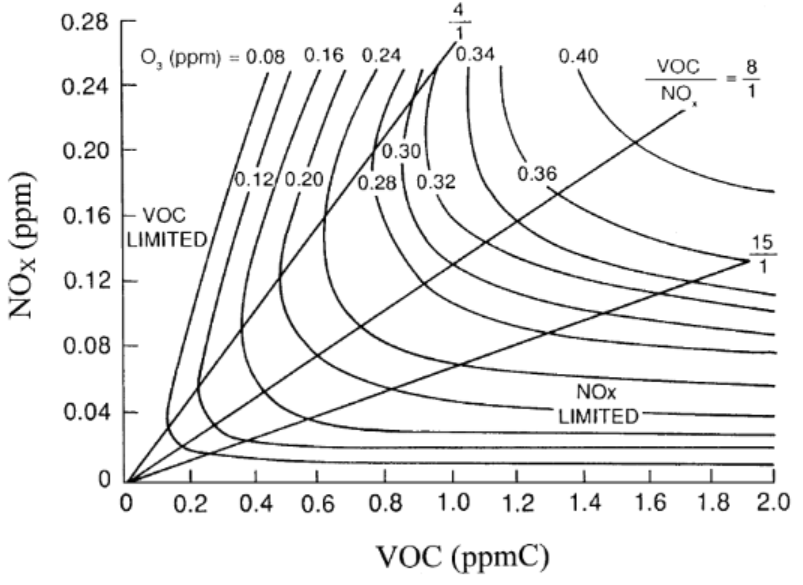
\includegraphics[width=.38\textwidth]{NOx-VOC_curve.png}
		\vspace{.2cm}
		\label{NO_x_VOC}
		}
	\subfloat
		{
		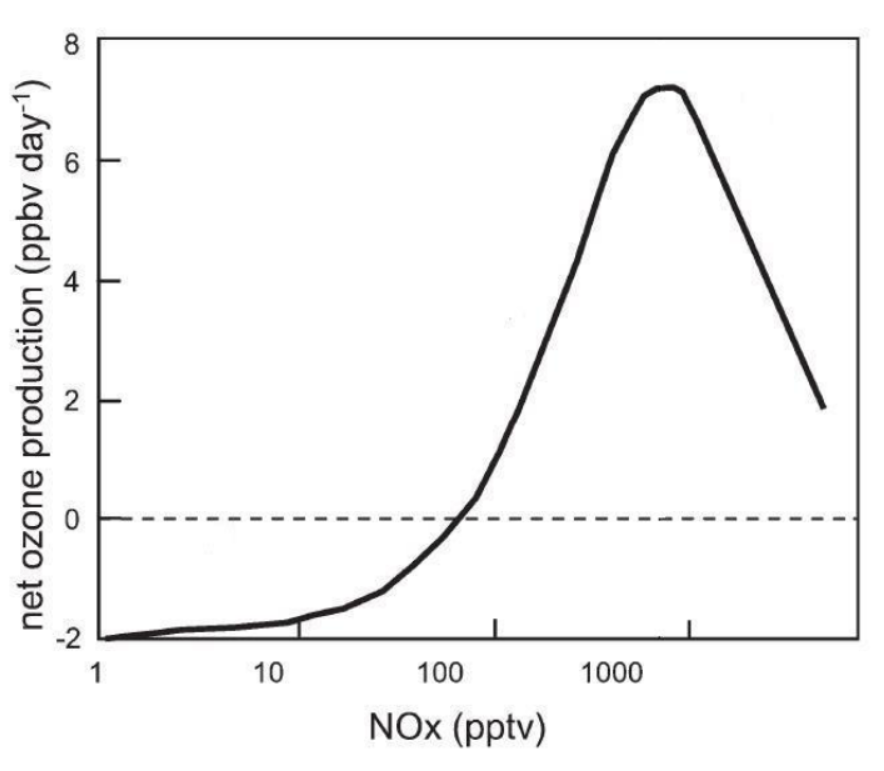
\includegraphics[width=.32\textwidth]{NO_x_ozone.png}
		\label{NO_x_ozone}
		}
	\caption{\textbf{(a)} Example isopleth diagram displaying peak ozone concentrations calculated from various initial concentrations of \ce{NO_x} and a specified VOC mixture, using the US EPA empirical kinetic model \cite{Dodge1977, Jenkin2000}. \textbf{(b)} Schematic representation of the variation of net ozone production efficiency with \ce{NO_x} concentrations, with magnitudes reflecting clean free tropospheric conditions (i.e. low VOC/\ce{NO_x} ratio) \cite{Monks2005}.}
	\label{}
\end{figure}

Figure \ref{NO_x_VOC} from Jenkin et al.\ (2000) \cite{Jenkin2000} is an exemplary ozone isopleth diagram that illustrates the \ce{O_3}-\ce{NO_x}-VOC relationship. At typical aircraft cruising altitudes (i.e. UTLS), where the emissions of \ce{NO_x} have a significant influence on atmospheric chemistry, it is likely that VOC content is very low relative to the background NO and \ce{NO_2} concentrations. Therefore, it is likely that typical VOC/\ce{NO_x} ratios are low in the UTLS, meaning that under the assumption of constant VOC concentrations, the \ce{NO_x}-\ce{O_3} relationship takes a form similar to figure \ref{NO_x_ozone}.

\subsubsection{Low-\ce{NO_x} regime}
In unpolluted environments characterised by low \ce{NO_x} concentrations, such as in regions where the ambient air is unperturbed by aircraft emissions, the dominant reaction pathway of OH is to react with CO (\textasciitilde75\%), with the remainder reacting with \ce{CH_4} \cite{Thompson1992}. The dominant reaction pathway therefore involves the oxidation of CO to form \ce{CO_2}, as in reaction \eqref{OH+CO} (for a detailed description of both the CO and the \ce{CH_4} oxidation cycles in low \ce{NO_x} conditions, see Wasiuk (2014) \cite{Wasiuk2014}). In this CO oxidation cycle, produced atomic hydrogen (H) then reacts with oxygen to form \ce{HO_2} \eqref{H+O2+M}, which subsequently reacts with \ce{O_3} to form OH in the background troposphere \eqref{HO2+O3}. This initiates a chain sequence in which OH and \ce{HO_2} interconvert through the termination of ozone \eqref{OH+O3}. This clean condition scheme therefore limits pollutant build up in the unpolluted upper troposphere and keeps ozone levels under control \cite{Jacob1999}.

\reaction[OH+CO]{OH + CO -> H + CO_2}

\reaction[H+O2+M]{H + O_2 + M -> HO_2 + M}

\reaction[HO2+O3]{HO_2 + O_3 -> OH + 2O_2}

\reaction[OH+O3]{OH + O_3 -> HO_2 + O_2}

Net reaction: \reaction[CO+O3->CO2+O2]{OH + CO + 2O_3 -> CO_2 + HO_2 + 2O_2}

Alternatively, \ce{HO_2} can react with itself to form hydrogen peroxide (\ce{H_2O_2}) \eqref{HO2+HO2}, or with organic peroxy radicals such as the methyl peroxy radical (\ce{CH_3O_2}) to form organic hydroperoxides \eqref{CH3O2+HO2}. These reaction pathways can become an effective sink for \ce{HO_x} under most conditions, because the formation of peroxides prevents further \ce{HO_x} interconversion \cite{Gunz1990}.

\reaction[HO2+HO2]{HO_2 + HO_2 + M -> M + O_2 + H_2O_2}

\reaction[CH3O2+HO2]{CH_3O_2 + HO_2 -> CH_3O_2H + O_2}

\subsubsection{\ce{NO_x}-limited regime}
In polluted environments, where \ce{NO_x} levels are raised considerably above ambient concentrations (e.g. typical aircraft cruising altitudes), CO oxidation takes place through reactions \eqref{OH+CO} \eqref{H+O2+M}, however in the presence of nitrogen oxides, ozone is produced rather than depleted. Peroxide formation reactions \eqref{HO2+HO2} and \eqref{CH3O2+HO2} compete with the oxidation of NO to \ce{NO_2} \eqref{HO2+NO} for available \ce{HO_2} concentrations. When the latter reaction prevails, \ce{NO_2} photolysis takes place, converting back to NO with ground state oxygen \ce{O(^{3}P)} forming as a byproduct \eqref{NO2+hv}. Subsequently, \ce{O(^{3}P)} reacts with atmospheric oxygen to produce \ce{O_3} \eqref{O3P+O2+M}.

\reaction[HO2+NO]{HO_2 + NO -> OH + NO_2}

\reaction[NO2+hv]{NO_2 + h\nu (\lambda $<$ 420 nm) -> NO + O(^3P)}

\reaction[O3P+O2+M]{O(^3P) + O_2 + M -> O_3 + M}

Net reaction: \reaction[CO+2O2]{CO + 2O_2 -> CO_2 + O_3}

Additionally, the methane oxidation cycle leads to net ozone production in the presence of \ce{NO_x}. The oxidation of methane by OH produces water vapour and the methyl radical (\ce{CH_3}) \eqref{OH+CH4}, which further reacts with oxygen to form \ce{CH_3O_2} \eqref{CH3+O2+M}. The produced methyl peroxy radical can then react with \ce{NO} to form \ce{NO_2} through reaction \eqref{CH3O2+NO}.

\reaction[OH+CH4]{OH + CH_4 -> H_2O + CH_3}

\reaction[CH3+O2+M]{CH_3 + O_2 + M -> M + CH_3O_2}

\reaction[CH3O2+NO]{CH_3O_2 + NO -> CH_3O + NO_2}

\reaction[CH3O+O2]{CH_3O + O_2 -> HO_2 + HCHO}

Net reaction: \reaction[CH4+2O2]{CH_4 + 2O_2 -> HCHO + O_3}

The methoxy radical (\ce{CH_3O}) produced can form additional \ce{HO_2} and formaldehyde (HCHO) through reaction \eqref{CH3O+O2}, which is then capable of reacting to form further \ce{NO_2} through reaction \eqref{HO2+NO}. The resultant \ce{NO_2} produced through reactions \eqref{CH3O2+NO} and \eqref{HO2+NO} consequently produces ozone through the same pathway as CO oxidation (i.e. \ce{NO_2} photolysis \eqref{NO2+hv} followed by reaction of the \ce{O(^3P)} photoproduct \eqref{O3P+O2+M}). The net reaction of methane oxidation in polluted environments therefore results in positive ozone production. Figure \ref{NOx-O3-CO-CH4} is a visual representation of the \ce{NO_x}-\ce{O_3}-CO-\ce{CH_4} oxidation reaction scheme described thus far.

\begin{figure}[H]
  \centering
  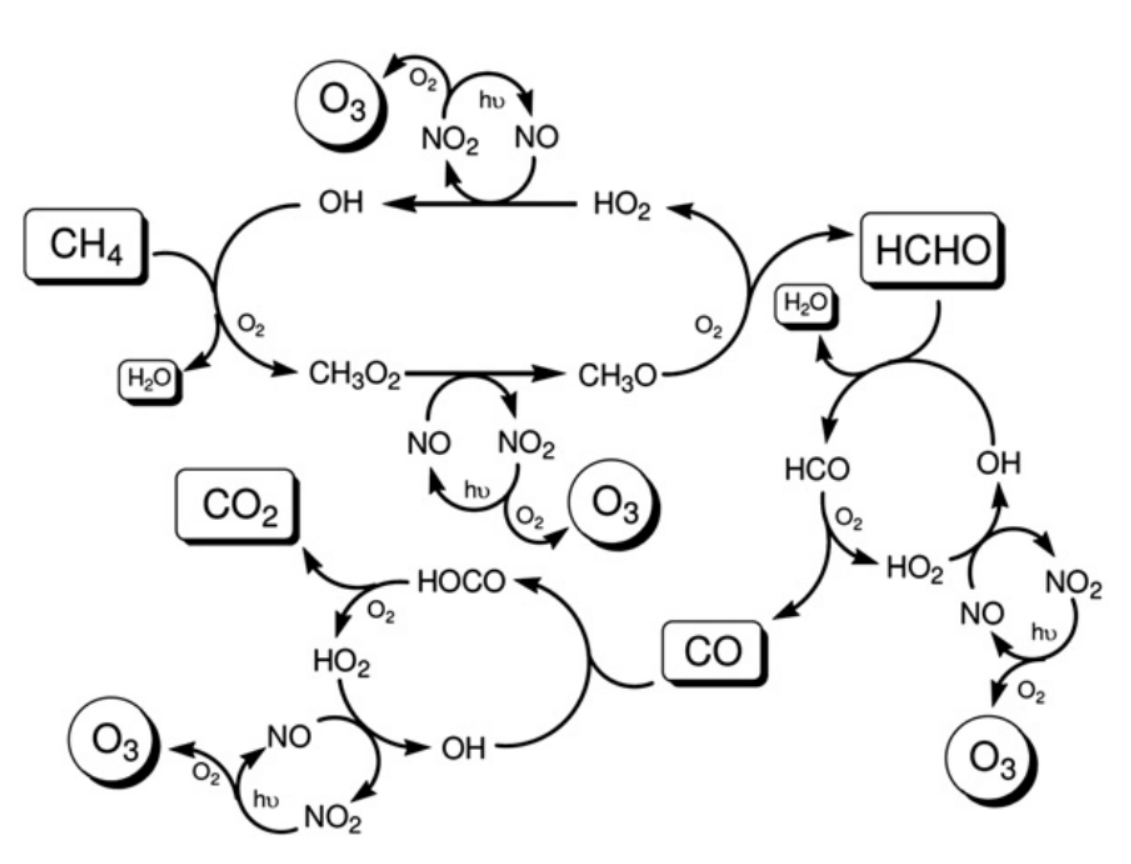
\includegraphics[width=0.65\linewidth]{NOx-O3-CO-CH4.png}
  \caption{Schematic representation of the OH initiated, \ce{NO_x}-catalysed oxidation scheme for CO and \ce{CH_4} \cite{Jenkin2008}.}
  \label{NOx-O3-CO-CH4}
\end{figure}


%The resultant \ce{NO_2} produced from reaction \eqref{} can then feed into the ozone formation cycle through \eqref{} and \eqref{}. Alternatively, the methoxy radical (\ce{CH_3O}) produced can form additional \ce{HO_2} and formaldehyde (HCHO) through reaction \eqref{}, which then produces further \ce{NO_2} through 

%Ozone role in oxidation of atmosphere. How it leads to warming. How aircraft NOx increases ozone production rate.

\subsubsection{\ce{NO_x}-saturated regime}
Under very high \ce{NO_x} conditions, such as inside aircraft exhaust plumes or in regions of the atmosphere where aircraft fly in close proximity and their corresponding emissions accumulate, the ozone production efficiency starts to drop off. This is because as NO and \ce{NO_2} surpass a threshold concentration, known as the compensation point (peak of the curve in figure \ref{NO_x_ozone}), they begin to compete with VOCs (e.g. methane) for reaction with hydroxyl (OH), organic peroxy (\ce{RO_2}) and peroxide \ce{RCO_3} radicals \cite{Wasiuk2014}. The products of these reactions are examples of nitrogen reservoir species: nitrous acid (HONO), nitric acid (\ce{HNO_3}), peroxynitric acid (\ce{HO_2NO_2}), peroxy nitrates (\ce{RO_2NO_2}) and peroxyacyl nitrates (\ce{RCO_3NO_2}). Reservoir species are much less efficient at forming ozone as they are more stable and are also more likely to get washed out of the atmosphere through depositional processes \cite{Jenkin2000}. They are also much more stable in the upper troposphere compared to the surface equivalent \cite{Khan2020}. Thus, reactions \eqref{NO+OH+M} to \eqref{NO2+RCO3+M} serve as termination reactions, removing radicals from the atmosphere and preventing additional ozone formation through conversion of \ce{NO_x} to its more stable counterparts.

\reaction[NO+OH+M]{NO + OH + M -> HONO + M}
\reaction[NO2+OH+M]{NO_2 + OH + M -> HNO_3 + M}
\reaction[NO2+HO2+M]{NO2 + HO_2 + M -> HO_2NO_2 + M}
\reaction[NO2+RO2+M]{NO_2 + RO_2 + M -> RO_2NO_2 + M}
\reaction[NO2+RCO3+M]{NO_2 + RCO_3 + M -> RCO_3NO_2 + M}

\ce{NO_x} saturation effects become particularly important to observe in the case of diluting aircraft exhaust plumes, because the high \ce{NO_X}-VOC ratio means that termination reactions are often favoured over catalytic ozone formation \cite{Song2003}. In the relatively fresh exhaust plume (first 10 minutes) where \ce{NO_x} concentrations are significantly enhanced, ozone titration by NO results in large scale production of \ce{NO_2} \eqref{NO+O3}, but decreases the formation of \ce{HO_x} due to depleted ozone levels in the plume.

\reaction[NO+O3]{NO + O_3 -> NO_2 + O_2}

The dilution of the plume results in reduced \ce{NO_x} concentrations over time, and the in-plume chemistry transitions from \ce{NO_x}-saturated to \ce{NO_x}-limited. With ozone levels still depleted, the remaining \ce{HO_2} and \ce{RO_2} in the plume (formed from the oxidation of CO and VOCs by OH) react with the remaining NO to produce OH and \ce{NO_2} without further depleting ozone. This leads to increasing OH and \ce{NO_2} concentrations which give rise to a net ozone recovery due to \ce{NO_2} photolysis (reactions \eqref{NO2+hv} and \eqref{O3P+O2+M}), with full recovery to ambient concentrations within 1--2~h post emission. As ozone levels rise in the plume back towards ambient concentrations, the photochemical formation of OH becomes more common, through reactions \eqref{O3+hv} and \eqref{O1D+H2O}. Newly formed OH can oxidise CO and VOCs to form peroxy radicals which catalyse ozone production, however it can also react with NO and \ce{NO_2} to form stable nitrogen reservoir species, through reactions \eqref{NO+OH+M} to \eqref{NO2+RCO3+M} \cite{Fritz2020}.

In the ID scenario inherent to large-scale climate models, ozone titration doesn't occur on the same scale due to lower mixing ratios of \ce{NO_x} when instantly diluted. Therefore, initial ozone depletion and subsequent recovery in the exhaust plume is not properly captured, meaning that instead, ozone levels remain reasonably high throughout and hence \ce{HO_x} production can remain stable. The stable \ce{HO_x} levels mean \ce{NO_x} to reservoir species conversion remains stable also, throughout the \ce{NO_x} lifetime. On a global scale, it has been shown that inclusion of plume processes leads to a net reduction in ozone forming potential of aviation \ce{NO_x} emissions. Vohralik et al.\ (2008) \cite{Vohralik2008} summarises the estimates made for the degree of reduction in ozone forming potential when plume effects were included. Initial findings from Kraabol et al.\ (2002) \cite{Kraabol2002} and Meijer et al.\ (1997) \cite{Meijer1997} estimated discrepancies in ozone production of 15--18\%, however these studies only accounted for ozone depletion in the plume, and not the \ce{O_3} generated during plume expansion. Inclusion of both ozone depletion and production in the plume in Meijer (2001) \cite{Meijer2001}, led to updated estimates in ozone formation changes 0\% to -5\% in January and +5\% to -10\% in July, indicating that plume processing can actually increase net ozone production when propagated to global scales. %Estimates from Fritz?

%The instantaneous dilution assumption inherent to large-scale climate models neglects the initial ozone depletion and subsequent recovery in the exhaust plume, hence omitting the in-plume \ce{NO_x} and \ce{HO_x} depletion, and therefore leading to a relatively constant ozone production rate throughout \cite{Fritz2020}. When propagated to global scales In Vohralik et al.\ (2008) \cite{Vohralik2008}, estimates for 

% Need to talk about different estimates for how much plume leads to overestimation of ozone

\subsection{Heterogeneous chemistry}
Reactions occurring in the atmosphere on either the gas--solid interface (e.g. aerosol particles) or the gas--liquid interface (e.g. cloud droplets) are referred to as heterogeneous reactions. The heterogeneous chemistry which can affect ozone concentrations through production and loss of \ce{HO_x} and \ce{NO_x} and the production of halogen radicals is extremely important in particle rich aircraft exhaust plumes and contrails \cite{Jacob2000}. The exhaust plume contains emitted soot particles and ultrafine aqueous aerosol particles which are either formed within the plume or entrained into the plume from ambient air, as elaborated on in the following subsection. In the case of contrail formation, heterogeneous chemistry becomes very efficient, due to the four-fold increase in particle surface area of contrail ice compared to typical exhaust and background aerosol surface area. Meilinger et al.\ (2005) \cite{Meilinger2005} states that the heterogeneous reactions occurring on aerosol particles have a negligible effect on ozone, however contrail ice can influence the ozone response to aircraft emissions by $\pm$0.5\% on a macroscopic scale which varies depending on time of day and year. Due to the relatively minor impact heterogeneous chemical reactions have on aircraft-induced ozone perturbations, and hence on aviation climate impact, their effect will be acknowledged, but the chemical intricacies will not be discussed further. For more information, see the references contained within this paragraph. 

%The effect of plumes on atmospheric photochemistry is shown to increase the soot, sulphate and water-ice surface areas for heterogeneous reactions which are important in defining ozone removal rates in the UTLS. \ce{N_2O_5} formed from the oxidation of \ce{NO_x} undergoes a reactive uptake on the plume species (e.g. water-ice surface), which results in \ce{HNO_3} formation. The reaction of \ce{N_2O_5} with HCl on ice results in \ce{ClNO_2} formation \eqref{N2O5+HCl->ClNO2+HNO3} which can compete with heterogeneous hydrolysis of N2O5 \eqref{N2O5+H2O->2HNO3}.
%
%\reaction[N2O5+H2O->2HNO3]{N_2O_5 + H_2O -> 2HNO_3}
%
%\reaction[N2O5+HCl->ClNO2+HNO3]{N_2O_5 + HCl -> ClNO_2 + HNO_3}
%
%The heterogeneous interactions are very important to the removal of \ce{NO_x} and \ce{HO_x} species during sedimentation events in the UTLS. These reactions can form reservoir species (e.g. \ce{HNO_3}, \ce{H_2O_2}) which can absorb onto sulphate aerosol and ice particles. Heterogeneous denoxification (reactions \eqref{N2O5+H2O->2HNO3} and \eqref{N2O5+HCl->ClNO2+HNO3}) and dehoxification (reactions \eqref{2HO2->H2O2+O2} and \eqref{2OH->H2O2}) lead to reduced concentrations of \ce{NO_x} and \ce{HO_x} which reduce the ozone production through gas-phase reactions \cite{Meilinger2005}.
%
%\reaction[2HO2->H2O2+O2]{2HO_2 -> H_2O_2 + O_2}
%
%\reaction[2OH->H2O2]{2OH -> H_2O_2}
%
%In the stratosphere, a number of heterogeneous reactions \eqref{ClONO2+H2O->HOCl+HNO3} to \eqref{HOBr+HBr->Br2+H2O} are important to various degrees on the surface of ice particles and saturated ternary solutions of water, HNO3 and H2SO4 in terms of ozone depletion on a global scale.
%
%\reaction[ClONO2+H2O->HOCl+HNO3]{ClONO_2 + H_2O -> HOCl + HNO_3}
%
%\reaction[ClONO2+HCl->Cl2+HNO3]{ClONO_2 + HCl -> Cl_2 + HNO_3}
%
%\reaction[ClONO2+HBr->BrCl+HNO3]{ClONO_2 + HBr -> BrCl + HNO_3}
%
%\reaction[HOCl+HCl->Cl2+H2O]{HOCl + HCl -> Cl_2 + H_2O}
%
%\reaction[HOCl+HBr->BrCl+H2O]{HOCl + HBr -> BrCl + H_2O}
%
%\reaction[BrONO2+H2O->HOBr+HNO3]{BrONO_2 + H_2O -> HOBr + HNO_3}
%
%\reaction[BrONO2+HCl->BrCl+HNO3]{BrONO_2 + HCl -> BrCl + HNO_3}
%
%\reaction[HOBr+HCl->BrCl+H2O]{HOBr + HCl -> BrCl + H_2O}
%
%\reaction[HOBr+HBr->Br2+H2O]{HOBr + HBr -> Br_2 + H_2O}
%
%The heterogeneous reactions initiated by \ce{ClONO_2}, HOCl, \ce{BrONO_2}, HOBr produce \ce{Cl_2}, BrCl, \ce{Br_2} which then yields Cl and Br radicals by photolysis. The heterogeneously activated Cl and Br can subsequently enhance ozone depletion \cite{Meilinger2005}.
%
%The extent of heterogeneous reactions \eqref{N2O5+H2O->2HNO3} to \eqref{HOBr+HBr->Br2+H2O} offset the effects of gas-phase reactions \eqref{NO+O3->NO2+O2} to \eqref{NO2+RCO3+M->RCO3NO2+M} on \ce{NO_x} initiated ozone formation which depends on a variety of chemical and dynamic factors (e.g. aerosol microphysics, atmospheric dynamics).

 \subsection{Aerosol and contrail microphysics}
\label{Microphysics}
Whilst the climate impact of aviation \ce{NO_x} emissions is dependent on the photochemical processes catalysing ozone production and methane destruction, the evolution and radiative forcing of aerosols and contrails is predominantly controlled by microphysical processes that occur at the aircraft plume scale. 

\subsubsection{The microphysical formation of aerosols and contrails}
Upon release into the atmosphere, aerosol particle formation occurs through one of two nucleation pathways: 

\begin{enumerate}
	\item The condensation of two distinct gas phase molecules to form a liquid phase droplet through what is known as binary homogeneous nucleation. This is the case for reactive sulphur emissions that get chemically oxidised into sulphuric acid (\ce{H_2SO_4}), which then condenses with water vapour to form \ce{H_2SO_4 / H_2O} droplets \cite{Perry1994}.
	\item The gas-to-particle conversion occurring on the surface of foreign particles is known as binary heterogeneous nucleation, often leading to a liquid coating that forms on the particle. For example, \ce{H_2SO_4 / H_2O} droplets can form a partial liquid coating around chemically activated soot in the aircraft exhaust plume through heterogeneous nucleation, leading to soot aerosol formation; a process that plays an important role in the formation of contrails \cite{Karcher1996a}.
\end{enumerate}

\begin{figure}[H]
  \centering
  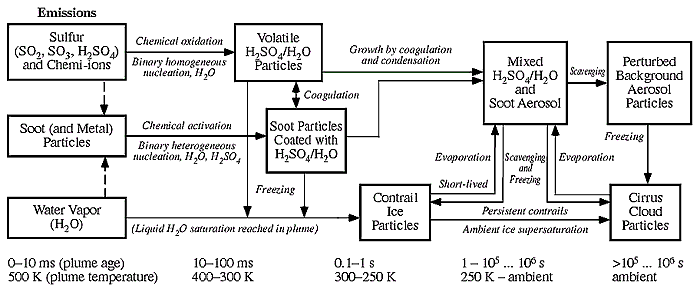
\includegraphics[width=0.95\linewidth]{Aerosol_fig.png}
  \caption{The microphysical formation of aerosol and contrail particles in an aircraft plume. Displayed as a function of plume age and temperature \cite{IPCC1999}.}
  \label{Microphys_IPCC}
\end{figure}

Newly formed aerosol particles subsequently grow in the aircraft wake due to further condensation by uptake of surrounding water vapour, and a process known as coagulation. Coagulation refers to the collision between particles that results in the formation of larger particles, often initiated by graviational settling, turbulence or thermal motion. A process called scavenging occurs when two particles, one much larger than the other, coagulate and lead to the removal of the small particle from its particular size category, with its mass contributing slightly to the increase in mass of the larger particle. Coagulation commonly occurs in aircraft wakes between volatile particles such as \ce{H_2SO_4 / H_2O} particles and soot aerosol, forming a mixed \ce{H_2SO_4 / H_2O}-soot aerosol (see figure \ref{Microphys_IPCC}). This sulphate-soot aerosol may eventually become scavenged by background aerosol particles if it remains stable for up to a day \cite{IPCC1999}. Alternatively, if at any point during the mixing process of aircraft exhaust with air, water-supersaturation is exceeded, aircraft-induced particles and entrained background aerosol can be activated into water droplets through the uptake of surrounding water vapour \cite{Karcher2018}. If temperatures are below threshold according to the SA criterion, then these aerosol-activated water droplets will freeze to form contrail ice particles in the aircraft wake on the order of seconds post emission. 

\subsubsection{Contrail microphysical properties}
The aforementioned microphysical processes (i.e. nucleation, condensation, coagulation, scavenging and freezing) determine the eventual composition and size distribution of particles in the aircraft wake, and if thermodynamic conditions permit, the formation and evolution of contrail ice particles \cite{AIR5715, Karcher2015}. Hereinafter, this section will focus on the microphysics of contrail ice particles, as they induce the most significant radiative response out of all aviation climate forcers. Findings from K{\"a}rcher et al.\ (1996b) \cite{Karcher1996b} conclude that the predominant ice nucleation pathway for contrail formation is heterogeneous freezing of chemically activated soot aerosol particles, as these are the only remaining particle type in sufficient abundance at the time of freezing. However, simulation results from K{\"a}rcher et al.\ (1998) \cite{Karcher1998} strongly suggest that contrail formation is still likely in the absence of soot and sulphur emissions, through the activation and freezing of background aerosols. 

The radiative forcing of contrails is thought to be determined by the product of optical depth and areal coverage \cite{Schumann2017}. In terms of areal coverage, contrail forcing is thus dominated by the presence of persistent contrails and contrail cirrus. However, the optical depth of a contrail is less dependent on its macroscopic properties and is instead determined by the optical and physical characteristics of the ice particles on the microscopic scale. The microphysical parameters deemed to be most responsible for inducing a radiative response are ice water content (amount of cloud ice per unit volume \cite{Karcher2018}), total ice particle number concentration, ice particle size distributions, effective radii, and ice particle shape \cite{Heymsfield2010}. Various studies have formulated methods to estimate RF and ERF from contrails, based on the parametrisation of these properties \cite{Meerkotter1999, Schumann2012a, Bickel2020}. It is defined that the optical depth is proportional to the ice water content divided by the effective radius of entrained ice particles \cite{Schumann2012a}. Contrails that tend to have more aspherical ice particle shapes are likely to have a stronger solar albedo, increasing the reflectance of the SW flux \cite{Meerkotter1999}. Ice number concentration is also thought to increase optical depth \cite{Karcher1999}. 

\begin{figure}[H]
	\centering
	\subfloat
		{
		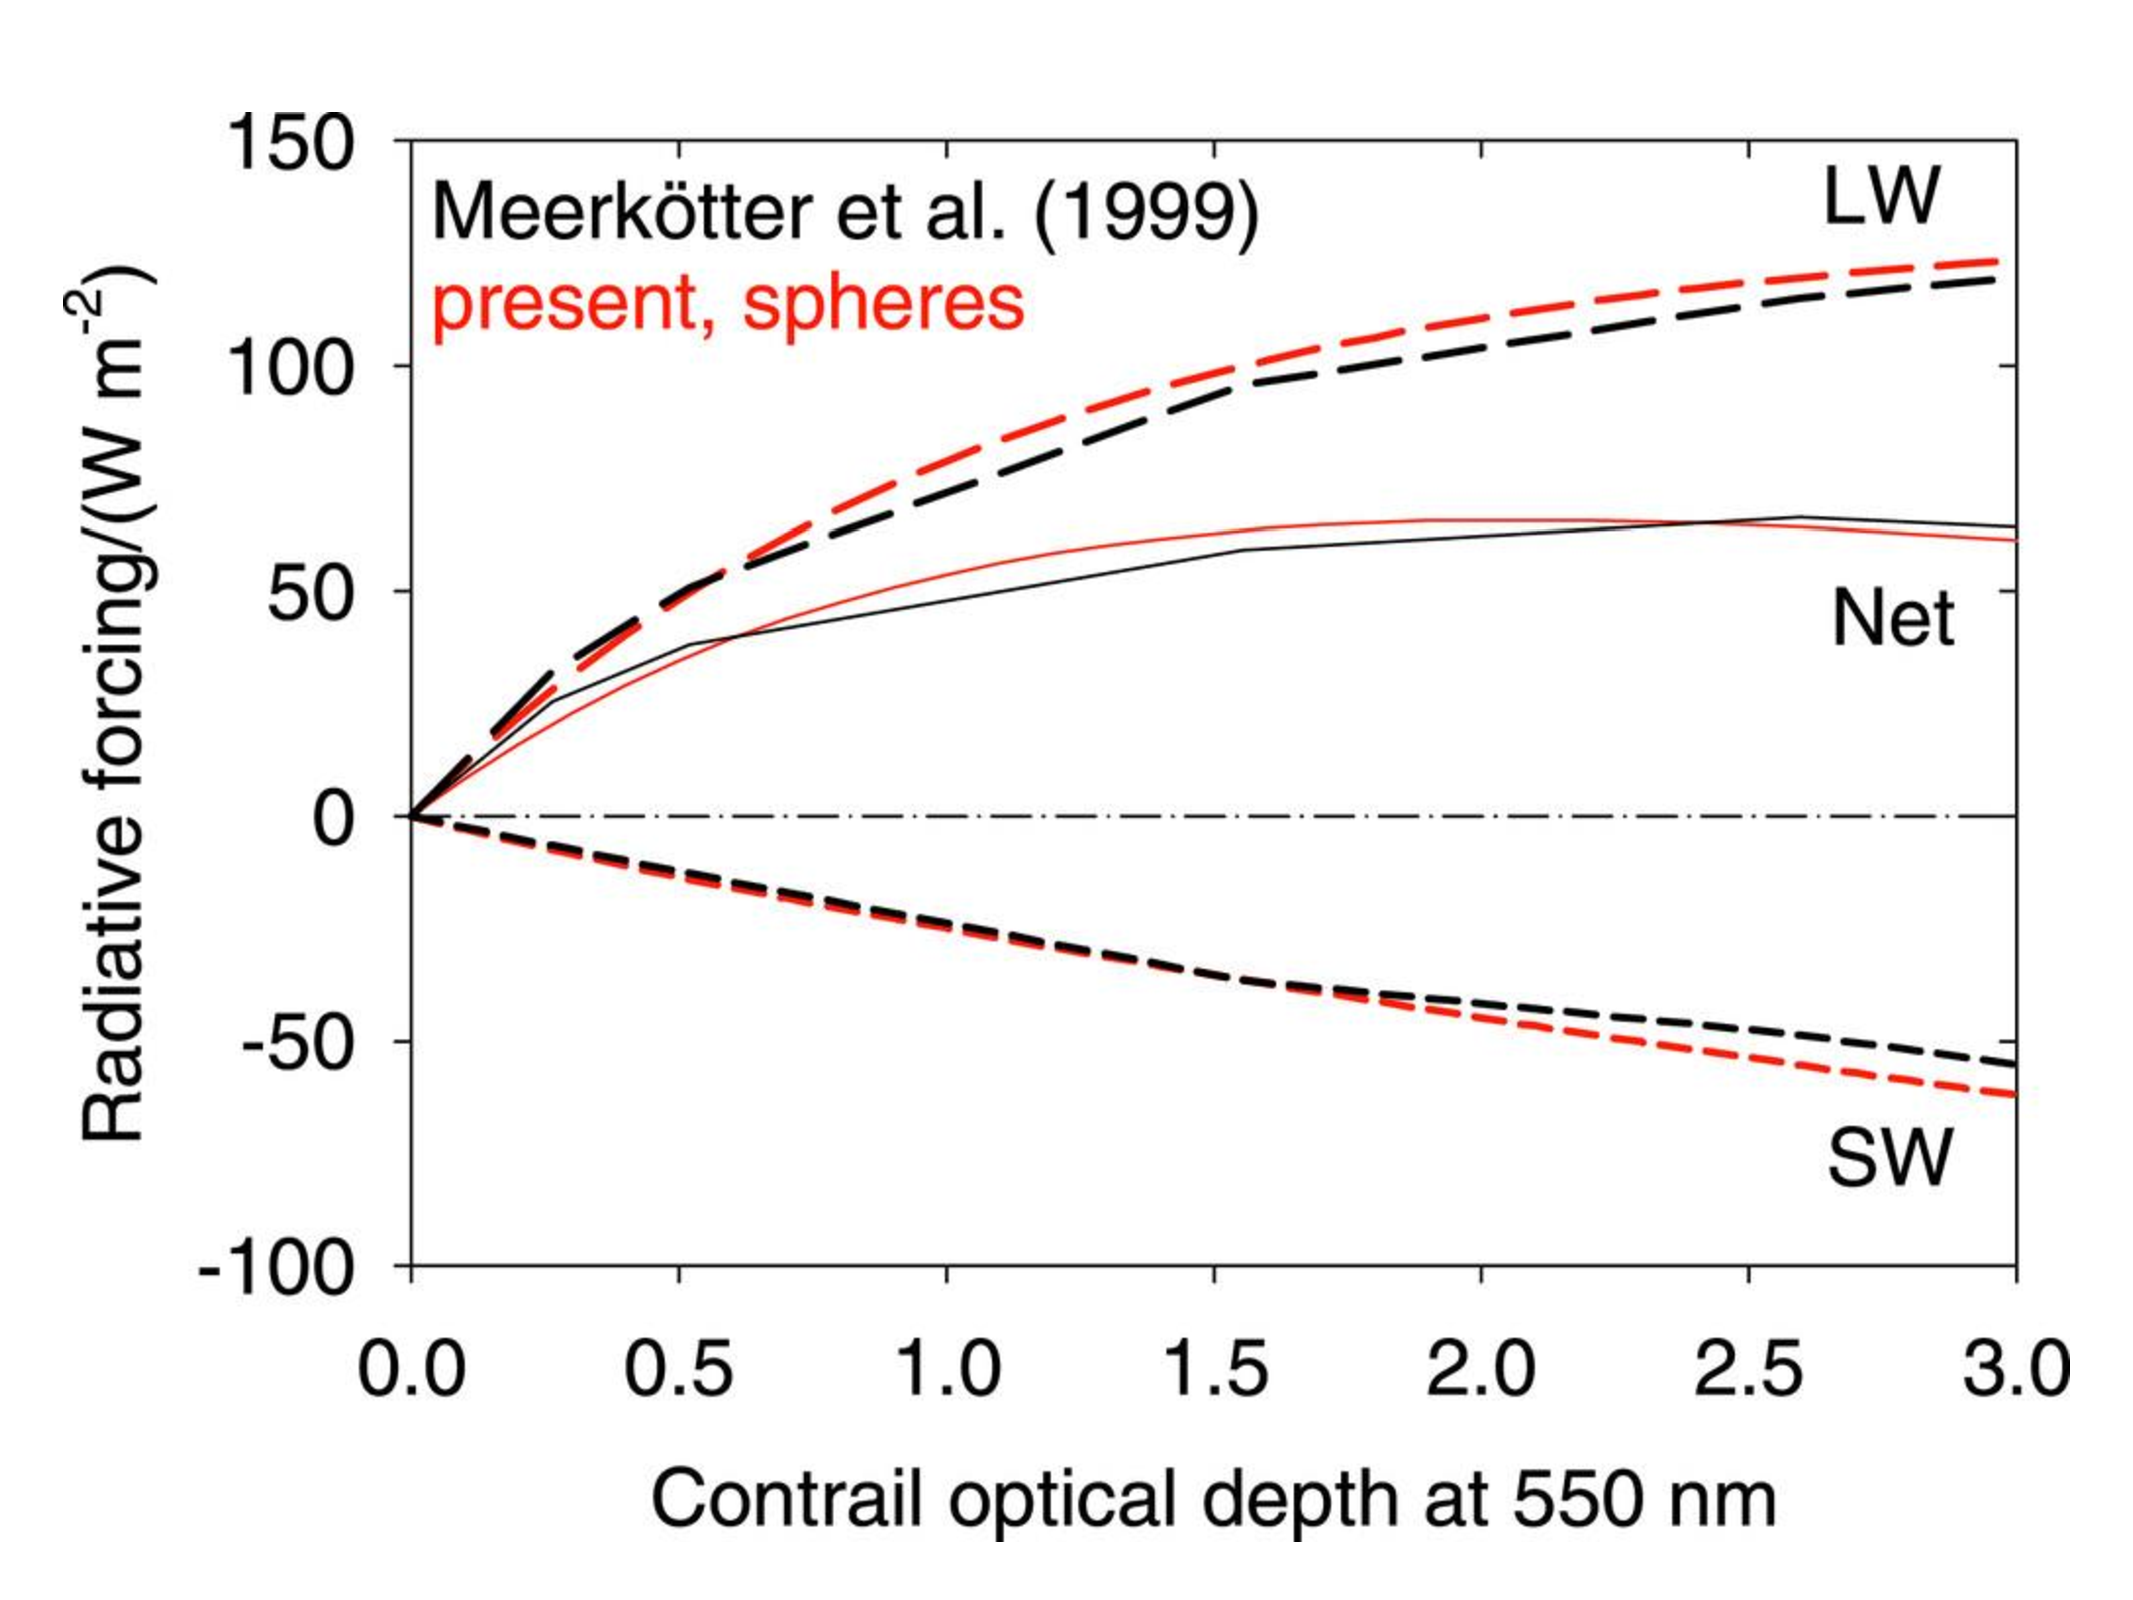
\includegraphics[width=.35\textwidth]{RFvsOD.pdf}
		%\vspace{.2cm}
		\label{RFvsOD}
		}
	\subfloat
		{
		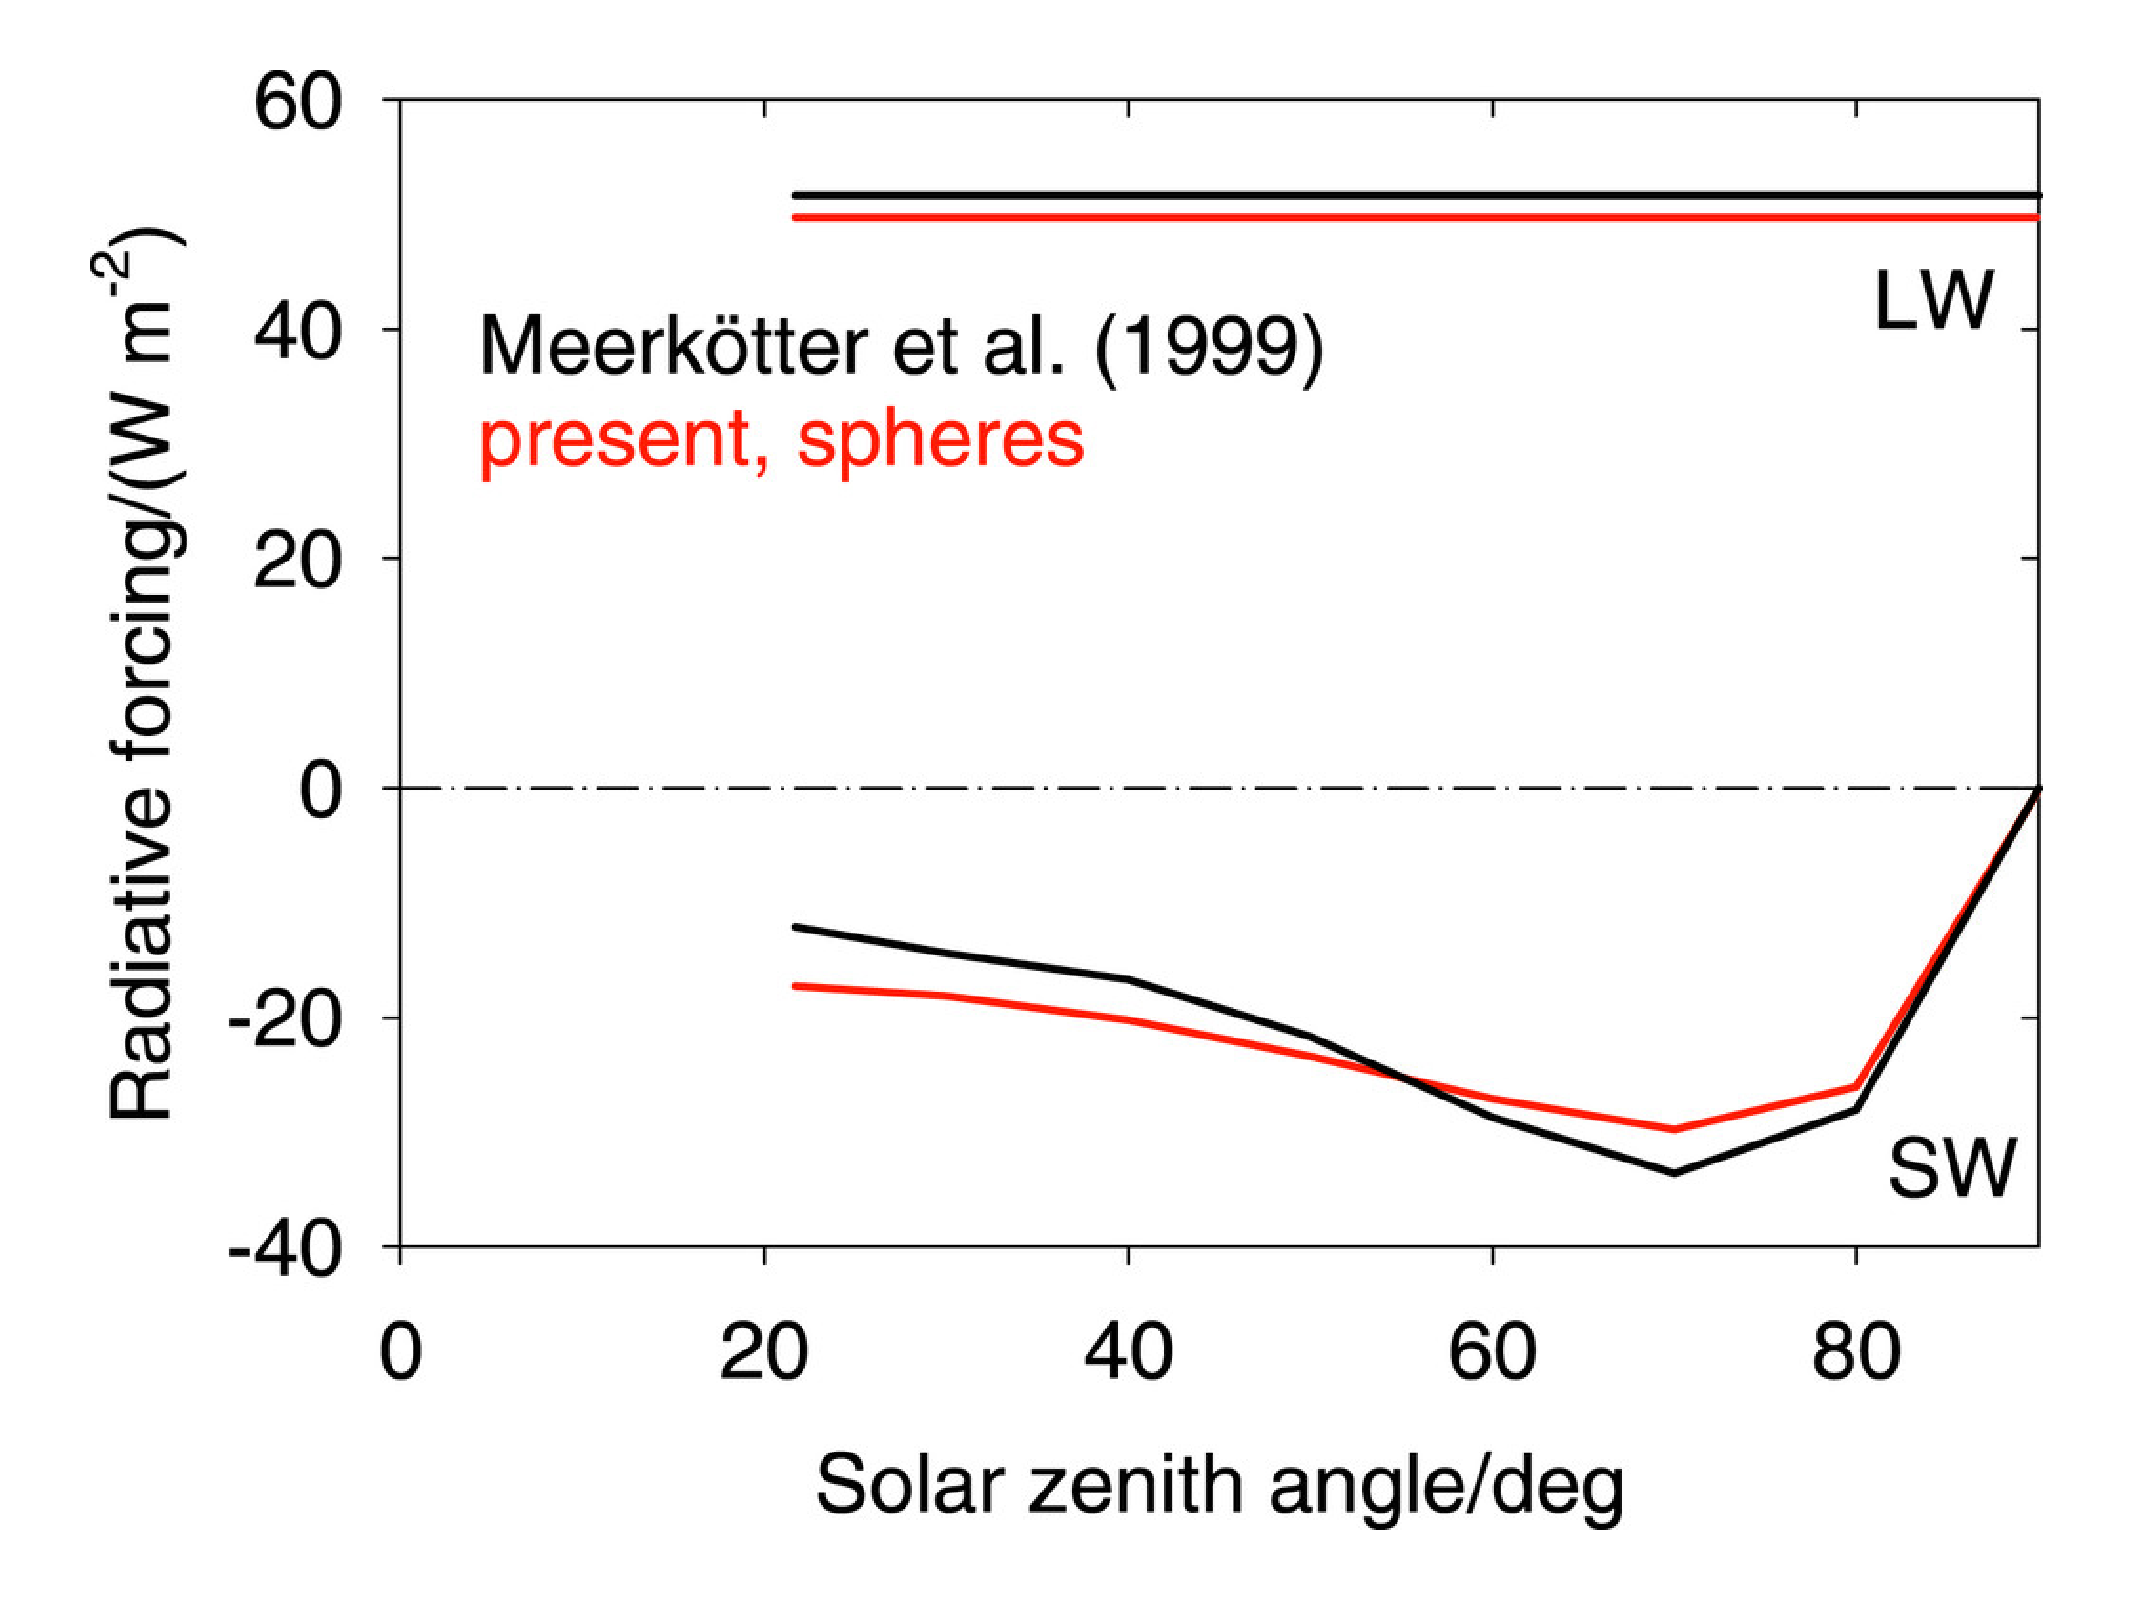
\includegraphics[width=.345\textwidth]{RFvsSZA.pdf}
		\label{RFvsSZA}
		}
	\caption{\textbf{(a)} Daily mean instantaneous SW, LW and net components of RF assuming 100\% contrail cover vs optical depth as calculated using the spherical ice particle model from Schumann et al.\ (2012b) \cite{Schumann2012b}. Results from Meerk{\"o}tter et al.\ (1999) \cite{Meerkotter1999} shown for comparison. \textbf{(b)} RF vs SZA for spherical ice particles, with Meerk{\"o}tter comparison shown. See Schumann et al.\ (2012b) \cite{Schumann2012b} for more detail on assumed atmospheric conditions.}
	\label{}
\end{figure}

Optical depth of contrail cirrus is generally seen to increase radiative forcing, however the relationship is nonlinear and under assumed atmospheric conditions \cite{Meerkotter1999, Schumann2012b}, contrail RF increases with optical depth up to around 2.0, where it peaks, before decreasing at higher optical depths (see figure \ref{RFvsOD}). This is due to the lessening increase of positive LW forcing with increasing optical depth, whilst negative SW forcing continues to drop at a similar rate throughout. In addition to contrail optical properties, the magnitude and direction of contrail forcing is also directly determined by solar position, otherwise known as the solar zenith angle (SZA) (see figure \ref{RFvsSZA}). Throughout the range of SZA values, LW forcing remains constant, because infrared emission from the Earth's surface is unaffected by solar flux. The SW flux on the other hand, goes further negative as SZA increases, up until a maximum at around 70\textdegree. Beyond this, the Sun begins to set and SW forcing returns to zero when the Sun is at 90\textdegree \ to the Earth's surface. This confirms the notion that contrails are solely warming at night, as the positive LW forcing always remains constant, whilst at night there is no chance of negative SW forcing.

%Sufficient understanding of the microphysical formation pathways for aerosols and contrail ice particles is therefore key in understanding their physical and optical properties, which directly determine their chemical and radiative impact on the atmosphere. Lack of integration of microphysical modelling is an issue that has been increasingly addressed in recent years, and 
% Need closing statements

\subsection{The saturation of aircraft emissions in high-density airspace regions}
\label{Saturation}
In dense airspace regions, where the frequency of traversing aircraft is high, the resulting exhaust plumes may intersect and overlap, further affecting the nonlinear atmospheric response to chemical and microphysical processing occurring at the plume scale. Two outstanding saturation effects documented in the literature include the surpassing of \ce{NO_x}-saturated conditions and the dehydration of surrounding water vapour due to contrail formation, leading to the mutual inhibition of ice particle growth in the aircraft wake.

\subsubsection{\ce{NO_x}-saturated conditions}
The accumulation of nitrogen oxide emissions in the troposphere due to overlapping aircraft plumes has been observed empirically. For example, Schlager et al.\ (1997) \cite{Schlager1997} witnessed \ce{NO_x} concentrations of up to 30 times the average background concentrations in the North Atlantic Flight Corridor, for an overlap of 2 to 5 aircraft plumes. As discussed in section \ref{Gas_phase_photochem}, the net ozone production rate in the upper troposphere is a nonlinear function of the concentrations of NO and \ce{NO_2}, with increasing \ce{NO_x} leading to increasing \ce{O_3}, up until a maximum, where any additional \ce{NO_x} serves to reduce ozone production efficiency (e.g. figure \ref{NO_x_ozone}). The turnover point, sometimes called the ``compensation point" is determined by competitive reactions involving nitrogen species and \ce{HO_x}. In the \ce{NO_x}-limited regime (left of the minimum ozone production efficiency \ce{P(O_3)_{max}}), NO drives the production of ozone through reaction with the hydroperoxy radical (\ce{HO_2}) \cite{Monks2005}. However, it also drives the removal of \ce{HO_x} through the reaction of OH with \ce{HO_2}, \ce{HNO_4} and \ce{NO_2}, thus limiting \ce{HO_x} available for further \ce{O_3} production \cite{Wennberg1998}. As \ce{NO_x} levels increase up to compensation point, the increasing competition of \ce{HO_x} removal processes begins to level off ozone production efficiency. Beyond this point, further increases in \ce{NO_x} serve to decrease \ce{P(O_3)}, thus signalling the start of the \ce{NO_x}-saturated regime. 

\begin{figure}[H]
  \centering
  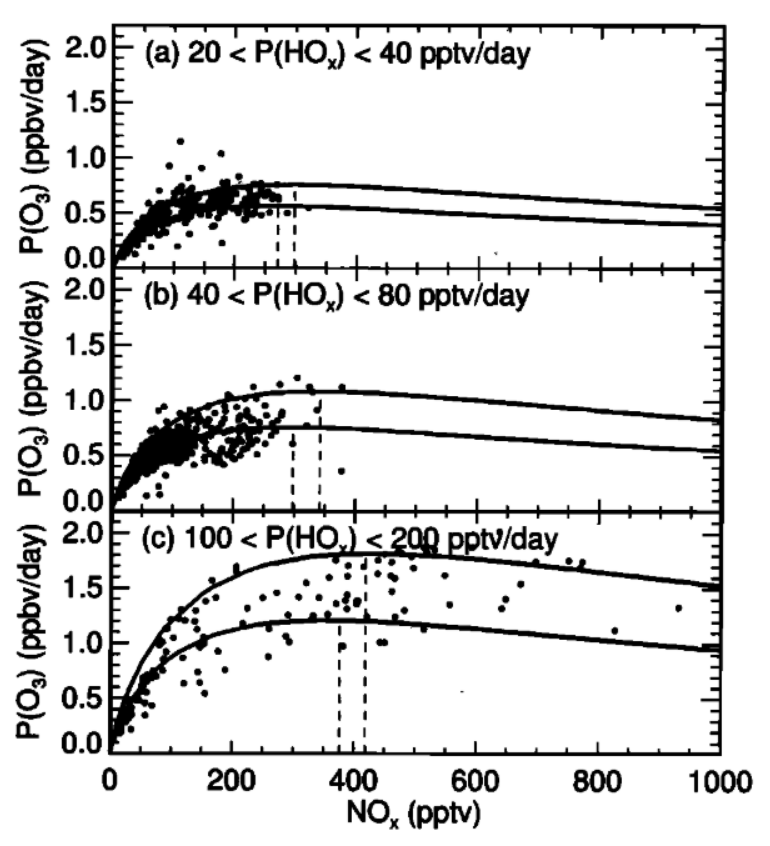
\includegraphics[width=0.5\linewidth]{Jaegle_sat.png}
  \caption{Empirical observations of ozone production rate as a function of \ce{NO_x} concentrations (parts per trillion volume, pptv), for three ranges of primary \ce{HO_x} production: (a) 20--40~pptv/day, (b) 40--80 pptv/day, and (c) 100--200~pptv/day. Solid lines represent the range limits from model calculations. Dashed lines depict the \ce{NO_x} level that induces peak ozone response \cite{Jaegle1999}.}
  \label{Jaegle_sat}
\end{figure}

During the POLINAT/SONEX campaign, Jaegl\'{e} et al.\ (1999) \cite{Jaegle1999} presented the first empirical evidence of \ce{NO_x}-saturated conditions in the NAFC. As seen in figure \ref{Jaegle_sat}, \ce{P(O_3)} levels increased with increasing \ce{NO_x} up until the saturation point, beyond which ozone production begins to drop off. 

As seen in figure \ref{Jaegle_sat} at 100--200~pptv/day of \ce{HO_x} production, \ce{P(O_3)} levels increased with increasing \ce{NO_x} up until around 300~pptv, where it is clear that \ce{NO_x} saturation has been reached. This means that any further emission of \ce{NO_x} under those specific atmospheric conditions will potentially serve to decrease the net ozone production rate. Generally speaking, ozone production efficiency, and hence the threshold for \ce{NO_x}-saturated conditions, is largely dependent on just two variables: the ambient \ce{NO_x} concentration (including the accumulation of \ce{NO_x} from lingering aircraft plumes) and the \ce{HO_x} production rate (which depends on the chemical composition of the atmosphere and the solar intensity \cite{Monks2005}) \cite{Jaegle2001}. 

Furthermore, model results from Kraabol et al. (2000b) \cite{Kraabol2000b} in a study observing interactions between plumes revealed that, for aircraft flying along the same track, plumes of follower aircraft exhibit a considerably smaller ozone response than that of the leader aircraft. This observation on a local scale opens up the discussion for controlled saturation of emissions through formation flight, to take advantage of effects that are beneficial to the climate.

\subsubsection{Dehydration effects due to contrail formation}
Contrails grow and persist in the atmosphere through deposition of water vapour from ice-supersaturated layers of the atmosphere. The conversion of atmospheric water vapour to solid phase ice particles has the potential to deplete local water vapour concentrations in regions conducive to persistent contrail generation \cite{Unterstrasser2010}. It is thought that the depositional growth of contrail cirrus in regions of high airspace density can even lead to the dehydration of \ce{H_2O} at typical flight levels, followed by the redistribution of humidity to lower levels, due to sedimentation and advection processes \cite{Schumann2015}. 

Contrail dehydration effects were first quantified by Burkhardt and K\"{a}rcher (2011) \cite{Burkhardt2011}, in which a global atmospheric model was used to perform long-term integrations of the global impact of contrail cirrus on natural cirrus reduction due to ambient water vapour depletion. The paper found initial RF estimates to be -7~\ce{mWm^{-2}}, lessening the contrail cirrus RF estimate by a factor of approximately one fifth, however the results were not conclusive. Schumann et al.\ (2015) \cite{Schumann2015} furthered this investigation through quantification of the impact of water exchange on contrail properties, large-scale humidity and the background climate. The results suggested that the drying at flight levels caused contrails to become thinner and last longer in the atmosphere, and the net reduction in contrail cirrus RF was deemed to be \textasciitilde15\% (not too dissimilar to the results of the Burkhardt and K{\"a}rcher (2011) \cite{Burkhardt2011}). Furthermore, the results from a second run of the model, with aircraft emissions enhanced by 100 times, showing increasingly significant dehydration effects due to contrail cirrus formation and the redirection of humidity to lower flight levels. This implies that local dehydration effects will be far more significant in dense airspace regions where emissions accumulate and contrails can overlap, such as over mainland areas and in flight corridors. Work by Unterstrasser \cite{Unterstrasser2010, Unterstrasser2020} has elaborated on this concept of local dehydration, through numerical analysis of contrail growth in close proximity flight scenarios. The studies conclude that aircraft contrails compete for available water vapour, mutually inhibiting growth and leading to a saturation effect which diminishes the contrail of subsequent aircraft travelling through that region. Under proposed formation flight scenarios, the total extinction (optical depth) and total ice mass behind a two-aircraft formation are found to be reduced by 20--50\% and 30--60\% respectively.

The presence of plume-scale effects that are amplified in close-proximity flight scenarios begs the question; can climate beneficial saturation effects such as \ce{NO_x}-saturated regimes and contrail-induced dehydration be exploited for mitigation purposes? Section \ref{Mitigation} explores the concept of formation flight and how these additional climate benefits from emissions saturation may provide further impetus for real-world implementation of these concepts.

\subsection{Parametrisation of plume-scale effects into global models}
Plume modelling methods serve as a useful tool for analysing the chemical and physical evolution of aircraft exhaust plumes throughout their lifetime. However, integrating high-resolution plume data into global atmospheric models is simply unfeasible when a large number of flights, on the order of 100,000--200,000 flights per day \cite{Flightradar24}, must be considered. To counteract this, simpler parametrisations of plume models are used, which capture so-called ``effective emissions" that attempt to correct the ID response of the large-scale model, according to the predicted plume-scale effects and their influence on the eventual climate impact. Parametrising plume-scale climate effects into global atmospheric models that assume instantaneous dispersion is a topic covered extensively in the literature, for both ozone-\ce{NO_x} chemistry \cite{Meijer1997, Paoli2020, Paoli2011, Cariolle2009} and contrail and cloud processes \cite{Burkhardt2009}. 

\subsubsection{Parametrisation of gas-phase chemical conversions}
In Paoli et al.\ (2011) \cite{Paoli2011}, three key concepts are reviewed which enable the parametrisation of nonlinear plume chemistry into ID global models; effective emission indices (EEIs), effective conversion factors (ECFs) and effective reaction rates (ERRs). 

The EEI concept was first theorised in Petry et al.\ (1998) \cite{Petry1998}, in an attempt to account for the difference in concentration evolution of key chemical species between large scale models which assume ID and plume models which account for the entrainment of emissions throughout the plume lifetime. EEIs provide a suitable correction to the original EI of an emitted species, so that the concentration is the same in both models at the end of the plume ``dispersion time" ${t_{\mathrm{ref}}}$, when emissions are fully dispersed into the dimensions of the computational grid cell in which they were released.  

Meijer (2001) \cite{Meijer2001} presents the concept of ECFs which are factors applied to the \ce{NO_x} emission index to account for the increased chemical conversion rate of \ce{NO_x} to nitrogen reservoir species in the plume. Since the total emitted reactive nitrogen (\ce{NO_y}) is chemically conserved throughout the plume lifetime, the amount of \ce{NO_y} throughout the plume lifetime is equal to the amount of \ce{NO_x} emitted initially, and hence the sum of ECFs for \ce{NO_x} and all reservoir species is unity \cite{Vohralik2008}. Thus, the faster in-plume conversion rates lead to a decreased \ce{NO_x} ECF, whilst the ECFs of reservoir species such as \ce{HNO_2} and \ce{HNO_3} increase considerably. As a result, the eventual net ozone production is affected as explained in section \ref{Gas-phase_photochem}, however ECFs vary considerably depending on altitude, latitude and seasonal variation meaning the magnitude and direction of the ozone perturbation is also affected.

% EEI and ECF figures

Despite the widespread use of EEIs and ECFs to parametrise plume-scale gas-phase chemical conversions in past literature, there are a number of known issues that affect accuracy such as mass conservation inconsistencies and poor accounting of local and regional variation in dispersion properties and turbulence. Cariolle et al.\ (2009) \cite{Cariolle2009} attempts to overcome such issues with the ERR concept. ERRs reconstruct the concentrations of the emitted species in the plume by diluting the emission to the resolution of the computational grids cell, while modified reaction rates are used to model reactions with ambient chemical species that occur at the plume scale. Modified reaction rates are introduced by the determination of effective reaction rate constants, which are used to compute secondary species produced in the plume. As a result, ERRs build on the EEI and ECF concepts by ensuring full mass conservation by modulating pre-existing background chemical cycles instead of directly estimating mass change, and they account for chemical transport due to diffusion and turbulence processes that are entirely dependent on location. 

% ERR fig

\subsubsection{Parametrisation of heterogeneous chemistry and microphysics}
Despite there being an extensive number of gas-phase chemistry parametrisations, the same cannot be said for parametrisations of heterogeneous chemistry and microphysics, for modelling aircraft plume-scale climate effects at a global scale. K{\"a}rcher et al. (1998) \cite{Karcher1998} was one of the first studies to explicitly attempt to parametrise heterogeneous reactions and aerosol microphysics in global models. The paper attributed the perturbations to the background aerosol layer (due to aerosol emissions from aircraft) to increasing surface areas and number concentrations of aerosol particles, which subsequently increase heterogeneous reaction rates. Findings from Meilinger et al. \cite{Meilinger2002, Meilinger2005} however, reveal that heterogeneous chemistry effects in dispersing aircraft plumes require special consideration of both the chemical and microphysical interactions, and the dynamical response of the plume itself. In Meilinger et al. (2005) \cite{Meilinger2005}, the Mainz Aircraft Plume Model is used to calculate the response of ozone and nitrogen reservoir species in the plume due to heterogeneous chemistry and microphysical effects. It is found from the modelling results that the impact of heterogeneous chemistry and microphysics on the ozone response at global scales is highly sensitive to local meteorology and the instantaneous state of the atmosphere. Therefore, parametrisation of these effects is much more convoluted than first thought, and due to the relatively minute impact on ozone response ($\pm$0.5\%), it is not unreasonable to disregard these effects in global modelling efforts.

Contrarily, the parametrisation of contrail microphysics into global models is of crucial importance, as contrail radiative forcing is determined primarily by the optical properties of its consituent ice particles. Burkhardt and K{\"a}rcher (2009) \cite{Burkhardt2009} summarise the parametrisations necessary to include contrail radiative forcing in global models; this includes parametrising the factors affecting ice supersaturation, contrail formation and persistence, contrail spreading and ice water content. This led to the development of the process-based contrail cirrus module (CCMod), which was later implemented in the global climate model ECHAM4, for global contrail cirrus radiative forcing analysis \cite{Burkhardt2010, Burkhardt2011, Lee2009}. More recently, a microphysical extension to CCMod was applied and implemented in ECHAM5 \cite{Bickel2020, Bock2016}. Model outputs were used to determine the global effective radiative forcing of contrail cirrus in Lee et al.\ (2021) \cite{Lee2021}, finding that the ERF is more than 50\% smaller than the RF equivalent. This is thought to be due to the reduction in natural cloudiness caused by contrail cirrus dehydration of the surrounding atmosphere, and due to the dependence of contrail climate impact on prevailing air traffic distribution patterns. See Lee et al. (2021) \cite{Lee2021} for more info on the parametrisations of contrail and aerosol microphysics implemented to deduce global ERF estimates.


%The \ce{NO_x} emission index is scaled such that the ratio of emission species $i$ to the emission of total reactive nitrogen (\ce{NO_y}) in the aircraft exhaust plume. 

%ECFs depend on assumed lifetime of the plume in the plume model. Difference in net chemical NOx prod and net chemical O3 prod between exhaust and ambient is largest in first few hours after emission. ECFs categorised by month, hourly emission, latitude, altitude. Sensitivity studies show this is a valid assumption.

%The plume model used to compute EEIs in this study is the SP model coupled with a chemistry mechanism known as CHEST (Chemistry Module for the Lower Stratosphere and Troposphere) \cite{}. Such a model requires consideration of atmospheric parameters and demands complex chemical and physical analysis at plume-scale resolution. Analysis of a large number of flights at such high complexity and fidelity is extremely demanding from a computational standpoint, and gives rise to issues surrounding resolving computations between plume models and global models \cite{}. Therefore, it is much more efficient from a large-scale perspective to apply effective emission corrections to aircraft emission inventories, accounting for nonlinear processing in the plume without vastly exceeding computational limitations.


%\subsection{Limitations to the plume modelling approach}
%Plume scale modelling of aircraft emissions is typically simulated using Eulerian 3-D atmospheric chemistry transport models to investigate its chemical impacts on the environment. However, this approach has also been recognised as a major uncertainty because emissions generally occur in plumes with scales much smaller than the grid resolution. Thus, this approach cannot explicitly capture the high initial concentrations of the chemicals within the plume. To overcome this, the Lagrangian models can be used in a domain-filling mode where the air parcels are distributed in the model domain proportionally to air density and each air parcel carries roughly the same mass of air. Interactions between neighbouring air parcels can be specified to represent mixing. In the grid cells with air flowing into the model domain, mass fluxes are accumulated with time and when the accumulated mass exceeds the mass of the air parcel, a new air parcel is released at a randomly chosen position at the boundary of the box. 

%The plumes in sub-grid scale arises an uncertainty due to the coarse grid resolutions of CTM model.  Such uncertainty can be improved by using grids with very fine resolution emissions and mixing. However, this can increase computational burden due to the large number of grid cells in the model domain as well as smaller time steps. Alternatively, a nested grid approach can be used with employing one or few fine grids over regions of special interest within larger domain. The multiple grid simulations can be performed simultaneously with two-way flow of information between the coarse and fine grids.


% Nested grid modelling


\section{Aviation climate impact mitigation}
\label{Mitigation}
It is customary practice among aviation policymakers to solely focus on mitigating the greenhouse effect induced by aviation carbon emissions. This means that analysis of the climate impact of non-\ce{CO_2} emissions is largely neglected, despite being responsible for over two-thirds of aviation-induced climate change \cite{Lee2021}. 

\subsection{Conventional \ce{CO2}-centric mitigation approach}
The industry fixation on aviation \ce{CO_2} mitigation stems from the easily quantifiable nature of the substance and its impacts; the direct coupling to fuel consumption and its relative stability and long lifetime make it a prime target for mitigation. This is due to the mutually assured reduction in both fuel consumption and corresponding \ce{CO_2} emissions, providing an economic and environmental incentive. Conventional mitigation approaches have often taken the form of improvements to aircraft and engine design, aviation technology and infrastructure, and aircraft operations, all aimed at minimising aircraft fuel consumption. These changes have been largely incremental due to the prioritisation of safety and economic stability over rapid implementation. As a result, efficiency gains have stalled in recent years (1--2\% per annum), whilst growth rates continue to rise unabated (4--5\% per annum) \cite{Peeters2016, Lee2021}. See figure \ref{eff_vs_growth} for a graphical representation of the trend in efficiency gains and aviation growth since 1940.

\begin{figure}[H]
	\centering
	\subfloat
		{
		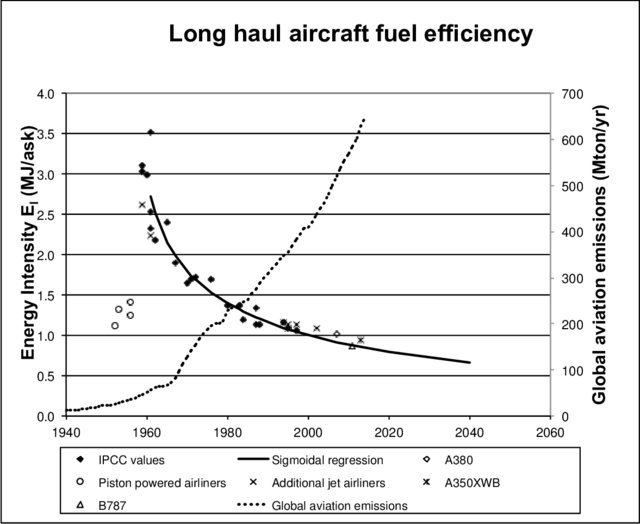
\includegraphics[width=.4\textwidth]{eff_vs_growth.jpg}
		%\vspace{.2cm}
		\label{eff_vs_growth}
		}
	\subfloat
		{
		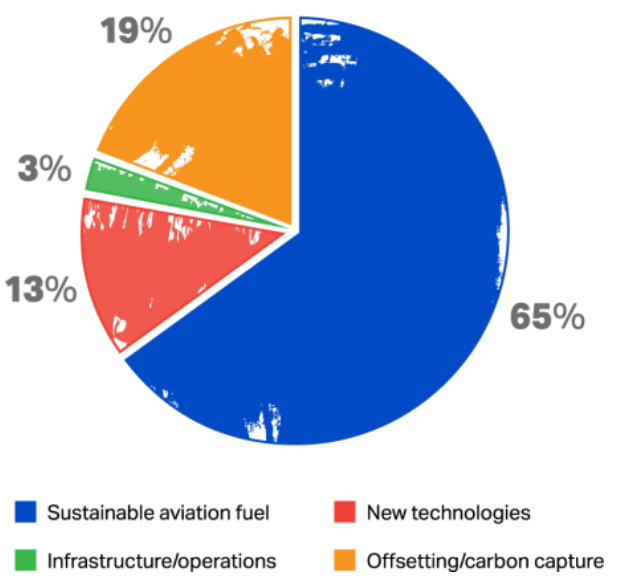
\includegraphics[width=.33\textwidth]{IATANetZero.png}
		\label{IATANetZero}
		}
	\caption{\textbf{(a)} Efficiency gains versus absolute aviation emissions growth since 1940 and projected to 2040 \cite{Peeters2016}. \textbf{(b)} IATA Net Zero 2050 contributions \cite{IATANetZero}.}
	\label{}
\end{figure}

At the International Air Transport Association (IATA) 77\textsuperscript{th} Annual General Meeting in 2021, a resolution was approved for the global air transport industry to achieve net zero carbon emissions by 2050, in accordance with the Paris climate agreement to limit global temperature rise to 1.5~\textdegree C \cite{IATANetZero}. This plan relies on the following contributions, as displayed in figure \ref{IATANetZero}: sustainable aviation fuels (SAFs) are to provide 65\% of the net carbon reduction, offsetting schemes and carbon capture are to deliver 19\%, new technologies such as hydrogen and electric propulsion to provide 13\%, and infrastructure/operational improvements to provide the final 3\%. This means that 78\% of the prospective net carbon emissions reduction comes from SAFs and alternative technology such as hydrogen and electric propulsion concepts. 

The fundamental issue with reliance on SAFs and nascent technologies, is that they may take decades to bring about noteworthy reductions in aviation climate impact. This is due to the need for a fleet-wide overhaul of aircraft equipment and associated ground infrastructure, which would likely incur huge costs and require extensive certification and approval processes \cite{ICF2021}. Not to mention, the environmental and ethical concerns have cast doubts over the prospect of a 4000 fold increase in global SAF production, to meet the IATA net zero target of 449 billion litres per year by 2050 \cite{IATANetZero, Henoi2022}. 

Carbon offsetting schemes, such as ICAO's Carbon Offsetting and Reduction Scheme for International Aviation (CORSIA), have been proposed to alleviate aviation climate impact in the meantime. However, an EU study investigating the efficacy of carbon offsetting indicates that such schemes often fall far short on providing meaningful mitigation, because of questionable offset quality, perverse incentives taking away from the real need to decarbonise, a lack of participation from key markets, and a clear lack of overall transparency and enforceability \cite{TandE2021, TandE2020}.

The remaining net zero contribution is expected to come from improvements to operations and infrastructure, which will continually provide 1--2\% per year. This will involve transitioning towards more efficient fuel management systems and improving overall technology and design of the aircraft, as well as advancing air traffic management systems and airspace modernisation \cite{Peeters2016}. However, as mentioned previously, improvements aimed at increasing aircraft fuel efficiency are largely outpaced by growth rates in passenger demand and hence emissions. Therefore, more must be done in the short term (i.e. the next 5 to 10 years), to reduce the dependency on nascent technologies which are still decades away from being impactful.

Whilst the proposed net zero targets are solely focused on decarbonising the aviation sector, it is inherently assumed that the reduction in non-\ce{CO_2} emissions will follow a similar trend. This review paper has evidenced however that this is not necessarily the case, due to the sensitivity of non-\ce{CO_2} emissions to combustor conditions, as well as the dependency of the atmospheric response on the environmental conditions of the ambient air. For this reason, action must be taken simultaneously to tackle non-\ce{CO_2} climate impact, alongside the current decarbonisation plan. with the potential to provide substantial climate impact reductions on a much shorter timescale.


%Global SAF production is currently only capable of providing ~0.05\% of total aviation fuel demand \cite{}, with a 4000 fold increase required to meet the net zero 2050 target \cite{IATA2050}. The prospect of upscaling SAF production at such a rapid rate has been overshadowed by feedstock supply and cost limitations, brought about by sustainability and ethical issues. This is due to the production of typical SAF feedstocks being (directly or indirectly) linked to ecosystem and biodiversity destruction, as well as detrimental impacts to low income and Indigenous communities, as reported in a landmark case study on the Omega Green refinery plant in Paraguay \cite{Henoi2022}. 


%Alternatively, the industry has looked towards longer term mass mitigation measures such as the implementation of sustainable aviation fuels (SAFs) and low carbon propulsion concepts such as hydrogen- or electric-powered flight. SAFs are renewable or waste-derived fuels that meet specific sustainability criteria laid out in ICAO Annex 16 Vol. IV \cite{Annex16}. These fuels typically have lower life-cycle \ce{CO_2} emissions of up to 70\% \cite{}, and also reduced PM emissions of soot and sulphate by 50-70\%, leading to alleviated contrail warming effects \cite{EASA2020, Voigt2021}. Such benefits are however, overshadowed by feedstock supply and cost limitations, which are largely brought about by issues related to sustainability and ethics. A recent landmark case study on the Omega Green refinery plant in Paraguay shed light on the tendency for typical SAF feedstocks to be directly or indirectly linked to ecosystem and biodiversity destruction and induces serious negative impacts on the local population, especially low income and indigenous communities \cite{Henoi2022}. Such findings cast doubt on the potential for the industry to increase SAF production by 4000 fold in the next 30 years, to achieve its contribution to the International Air Transport Association (IATA) Net Zero 2050 pathway \cite{IATAFlyNetZero}.

% Specify that elec and (green) hydrogen are best prospects for future low carbon flight
% Elec more suitable for short haul (find limitations and range) and hydrogen more for mid to long haul routes.
% EIS dates.
% Infrastructure and equipment overhaul and significant investment required to bring to fruition - IPCC need to begin decarbonising right now!

%Based on recent research relating to the need for developed nations to decarbonise fully by 2034 to retain a prospect of 50:50 chance of remaining within the 1.5°C emissions budget \cite{}, sole reliance on a low-carbon fuels strategy to mitigate UK aviation emissions is insufficient. As such, additional mitigation measures must be incorporated into the strategy in the interim to promote fleet-wide low-carbon flight. This is to increase the likelihood of limiting aviation’s climate contribution to 1.5°C, or at least below 2°C. 

\subsection{Alternative non-\ce{CO_2}-focused mitigation approach}
There are myriad solutions to mitigating aviation climate impact in the interim to low-carbon flight, however the focus here will remain on near-term operational mitigation measures that optimise aircraft routing by minimising non carbon-based radiative effects. 

As alluded to in sections \ref{emissions} and \ref{climate}, non-\ce{CO_2} emissions are on the other hand, produced in varying quantities depending on combustor conditions. Also, when released into the atmosphere, they have a spatio-temporally sensitive climate response, which depends on the background atmospheric conditions into which they are emitted. As such, anthropogenic as well as natural perturbations to atmospheric chemistry need to be considered; the entrainment of emissions to the exhaust plume for several hours post emission, leads to locally elevated emissions concentrations. This causes reactive non-\ce{CO_2} species to experience nonlinear chemical and microphysical processing that occurs at the scale of the plume, which subsequently affects their net climatic response when propagated to global scales.

Measures such as climate-optimal aircraft routing and formation flight present the potential for a substantial climate impact reduction in a relatively short timeframe, whilst requiring minimal technology changes to the current fleet and ground infrastructure.


\subsubsection{Climate-optimal aircraft routing}
The first measure proposed to tackle aviation’s non carbon-based environmental impact is climate-optimal aircraft routing. This involves re-routing aircraft in flight to avoid regions of the atmosphere that are particularly sensitive to non-\ce{CO_2} climatic effects, such as where \ce{NO_x} gives rise to excessive ozone production or where persistent contrails are formed. Simulation efforts have suggested that this method has the potential to reduce aviation climate impact by 10-20\%, at the cost of only a few percent of additional fuel consumption \cite{Grewe2014, Luhrs2016, Niklass2019a}. Moreover, the non-\ce{CO_2} climate impact from aviation is not evenly distributed across all flight distances, meaning that operational mitigation can be targeted towards flights which induce the most significant impact. For example, in a case study on contrail avoidance strategy \cite{Teoh2020}, it was found that diverting 1.7\% of the aircraft fleet could reduce the contrail climate impact by 59.3\%, with only a 0.014\% increase in fuel burn and accompanying additional \ce{CO_2} emissions. This sheds light on the sheer potential for significant reduction in aviation climate impact, through a minimally invasive climate-focused route optimisation strategy.

\begin{figure}[H]
  \centering
  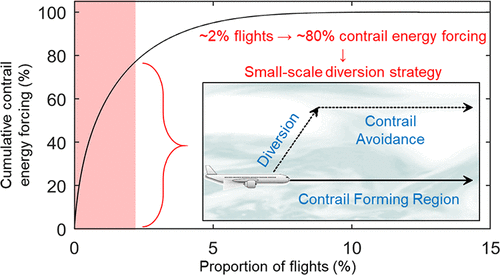
\includegraphics[width=0.7\linewidth]{Teoh.png}
  \caption{Schematic representation of contrail avoidance strategy. Plot of cumulative contrail energy forcing against proportion of flights \cite{Teoh2020}.}
  \label{Teoh}
\end{figure}

Implementation of this method in the real world does however require a number of issues to be addressed; Grewe et al. (2017) \cite{Grewe2017} lay out four key hurdles that must be overcome: 

\begin{enumerate}
	\item The accuracy and robustness in determining eco-efficient flight trajectories must be improved, and this must be possible near real time.
	\item Consensus must be achieved on determining the extent to which cooling effects should be exploited (e.g.\ intentionally flying a route that generates a cooling contrail could be seen as unnecessary intervention in nature).
	\item The implications of fleet-wide climate-optimal routing on the air traffic management system must be assessed rigorously, to ensure safety, order and efficiency is maintained.
	\item A non-CO2 market-based measure or policy pathway must be adopted to incentivise this transition towards a climate-optimised air traffic network.
\end{enumerate}

In the time since, a dedicated network of researchers from various institutions have been working towards bringing this concept to fruition on a large scale. The FlyATM4E research group has been developing methodologies to increase robustness in the determination of eco-efficient flight trajectories using so-called algorithmic climate change functions (aCCFs) \cite{Matthes2020}. Live trials are currently ongoing in the Maastricht Upper Area Control (MUAC) to investigate the operational feasibility of contrail prevention from an air traffic control perspective \cite{MUAC2021}. The inclusion of non-\ce{CO_2} effects of aviation in the European Union emissions trading scheme (EU ETS) and under CORSIA has also been discussed in great detail in a comprehensive report by Nikla{\ss} et al. (2019b) \cite{Niklass2019b}. Most recently, a comprehensive survey paper was published by Simorgh et al.\ (2022) \cite{Simorgh2022}, detailing the current operational strategies that are proposed in the state-of-the-art literature published in this field over the last few decades. The aim of this review was to collate methodologies used for aircraft performance modelling, climate modelling and optimisation, and to identify gaps to guide future research.

%Newinger and Burkhardt (2012) \cite{Newinger2012} explored the potential for mitigation of nighttime contrail forcing through air traffic scheduling adjustments. They proposed...


%Mention alt fuels, alt propulsion, technological changes etc. and say how they are long term due to infrastructure overhaul and large investment. Operational mitigation strategies require minimal change to current system, only operational changes which can be implemented without much additional investment. Just need more research and 

\subsubsection{Formation flight}
\label{Formation_flight}
Formation flight for wake energy retrieval involves the flight of two or more aircraft, with the follower aircraft positioned in the smooth updraft of the leader aircraft’s wake. This has been demonstrated in simulation \cite{Venkataramanan2003, Bangash2004} and flight testing \cite{Hanson2002} to reduce required lift and thrust of the trailing aircraft and offer a 5--10\% reduction in fuel burn in paired formation. Most work to date focuses on two-aircraft configurations, however three \cite{Bower2009} and more have also been considered. In figure \ref{Marks}, it is evident how this concept is used in practice to obtain aerodynamic benefits. The counter-rotation of the wake vortices of the leader aircraft leads to a stream of upwash on the outside of either rolled up vortex. Flying a follower aircraft in this region of upwash induces a vertical velocity, with aerodynamic benefits achieved at distances as much as 30 wingspans (i.e. \textasciitilde1~km for Airbus A320).

Safety is a critical hurdle, particularly in close formation cases, along with regulatory and air traffic systems and processes. Airbus' fello’fly wake energy retrieval project has undertaken initial work to identify and address operational and safety challenges, proposing regulatory standard adaptations to facilitate adoption, and conducting a trial transatlantic flight in 2021 \cite{Airbus2021}. Claims in this document state that formation flight strategies could be deployed around the middle of this decade. Proposed longitudinal separation distances for formation flight range from 56~ft \cite{Hanson2002} to 1.5~NM \cite{Airbus2021}, with lateral distances ranging from 10\%-span overlap to 30~m separation showing benefit. Routing aircraft into formation has been considered in simulation \cite{Xu2014}, with net fuel (and hence \ce{CO_2} saving benefits of 5.8\% being identified for a single operator, rising to 7.7\% for a transatlantic alliance. Significant benefits have been projected for long-haul and transatlantic routes, with more modest reductions for low-cost airline cases \cite{Kent2020}. 

% How many aircraft in transatlantic alliance??

\begin{figure}[H]
  \centering
  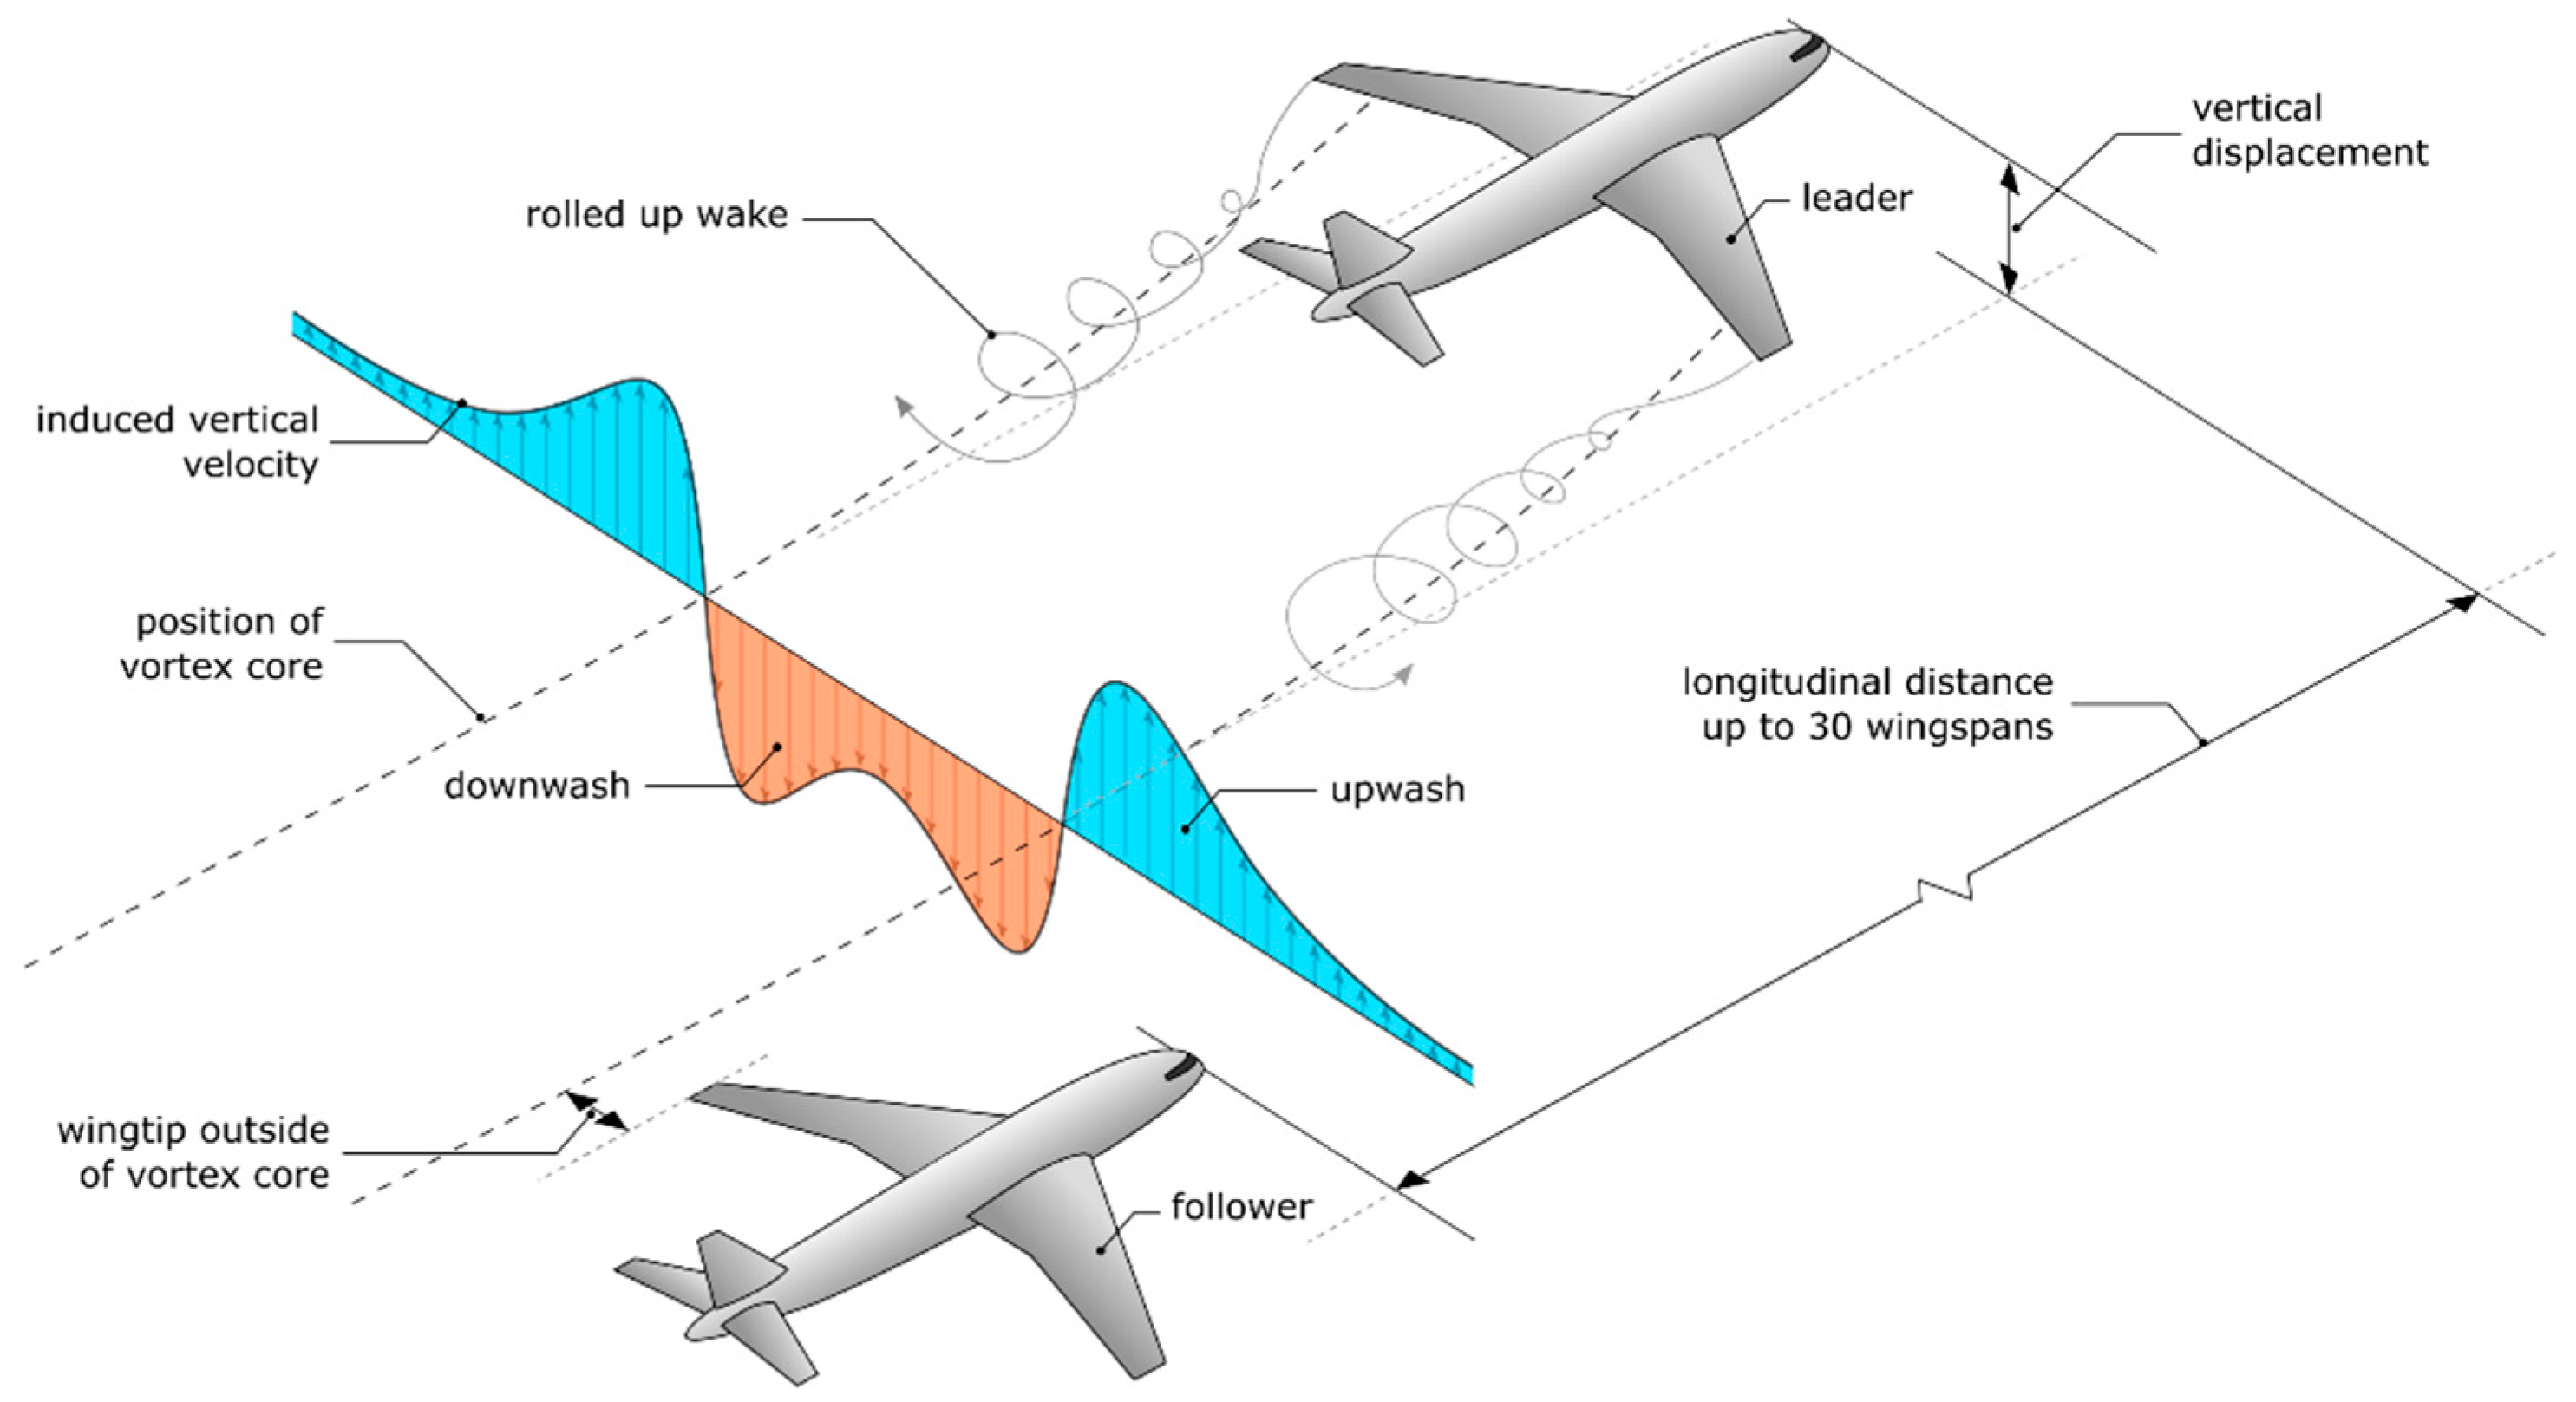
\includegraphics[width=0.8\linewidth]{FF.png}
  \caption{Visual representation of the formation flight concept, depicting the fundamental principles of wake energy retrieval \cite{Marks2020}.}
  \label{Marks}
\end{figure}

Non-\ce{CO_2} impacts have been neglected until recently, but a synergistic outcome of formation flight is realised via the saturation of emissions in the trailing exhaust plumes, leading to the aforementioned nonlinear chemical and microphysical response that reduces ozone and contrail formation, as detailed in section \ref{Saturation}. This has been projected to offer net climate impact reduction for a two-aircraft formation of 13--33\% \cite{Dahlmann2020}, which is significantly higher than the \ce{CO_2}-focused formation discount factors employed in the routing simulations mentioned above. Given the near-term feasibility demonstrated in industry-led trials, and the combined \ce{CO_2} and non-\ce{CO_2} benefits that produce an outsized impact when overall ERF is considered, formation flight offers a promising interim solution that can continue to be employed for drag reduction/wake energy retrieval once SAFs and hydrogen/electric propulsion are more widespread.

In this section, the prospects of non carbon-based operational mitigation measures have been discussed, and their potential to reduce aviation's net climate impact has been investigated. Gradual efficiency gains are unable to outpace the rapid growth in demand year upon year, meaning that more radical approaches must be implemented in order to achieve net zero emissions targets. For this reason, two concepts have been proposed and discussed: climate-optimal aircraft routing and formation flight. The former aims to re-route the aircraft to minimise time spent in particularly climate sensitive regions of the atmosphere, whereas the latter aims to optimise atmospheric conditions artificially by overlapping aircraft plumes and saturating local concentrations of emissions to lead to climate-beneficial effects. For the industry to truly reap the benefits and maximise potential non-\ce{CO_2} reductions from implementation of these measures, there is the potential to perform them simultaneously, in a controlled and safe manner. This would involve flying aircraft in formation, along routes which are optimised with respect to minimum climate impact.  





%Formation flight involves the flight of two or more aircraft in aerodynamic formation, with the follower aircraft positioned in the smooth updraft of the leader aircraft’s wake, reducing required lift and thrust, hence reducing fuel and CO2 emissions by 5-8\% per trip \ref{}. A fortuitous outcome of formation flight is however, the saturation of emissions in the trailing exhaust plumes, which can lead to the aforementioned nonlinear chemical and microphysical response that reduces ozone and contrail formation. The non-CO2 climate effects of a twin-aircraft formation flight are observed in \ref{}, where a climate model was used to determine the changes in NOx-related ozone production and contrail formation processes. The case study found that, despite a 1-3\% increase in flown distance, CO2 was reduced by 6\% and NOx was reduced by 11\%. This resulted in a 5\% reduction in ozone production efficiency due to NOx  saturation and a 48\% contrail reduction due to mutual competition for available water vapour, resulting in a total climate impact reduction of approximately 23\%. While part of the alleviated climate impact can be related to the decrease in total emissions due to wake energy retrieval of the follower aircraft, there is also further emphasis due to the saturation of emissions in the overlapping plumes of both aircraft involved. This demonstrates great potential for reducing both CO2- and non-CO2-induced climate effects from aviation, if such a scheme were to be carried out on a global scale.

%\subsubsection{Climate-optimal aircraft routing}
%Fleet-wide implementation of formation flight would however, pose a number of research obstacles, that must be overcome to maximise its cost-benefit potential, whilst ensuring the safe and orderly operation of aircraft in controlled airspace. Optimising aircraft trajectories to minimise fuel burn requires the consideration of nonlinear aircraft performance, wind and weather, payload, fuel load, and constraints set out by air traffic control \cite{}. Formation flight adds another variable to the fuel burn optimisation problem, maximising the time spent flying in formation whilst minimising deviation from the true optimal route. This is a research topic covered extensively in the literature \cite{}. Optimising formation flight trajectories to minimise climate impact on the other hand, is a relatively novel concept, which requires deeper understanding of the sensitivity of the climate response to emissions under a range of different atmospheric states. 



%Optimising a flight to minimise fuel burn very rarely results in minimum climate impact. This is because of the presence of climate-sensitive regions of the atmosphere where aircraft emissions have a higher climate impact per 

%\subsection{Alternative propulsion technologies}
%In recent years, new aircraft propulsion systems are being developed to operate on alternative aviation fuels (e.g. bio-jet fuels, electric, hybrid electric, hydrogen) which can significantly reduce both the CO2 and non-CO2 emissions from aviation sector (Voskuijl et al., 2018; Schafer et al., 2019). However, it is important to understand the technical, environmental and economic performance of these alternative fuels and the subsequent propulsion technologies for the broad application of these fuels. 
\section{Conclusions}
This review paper delivers a holistic overview of literature pertaining to the spatio-temporal climate sensitivity of the atmosphere to reactive non carbon-based species. This includes literature from a range of research areas: aircraft emissions, plume dispersion and dynamics, the distribution of air traffic and corresponding emissions, the climate impact of aviation on both a global and a local scale, and lastly the mitigation potential for both \ce{CO_2} and non-\ce{CO_2} climate impact. 

The generation of aircraft emissions firstly requires consideration and modelling of aircraft performance, to determine fuel consumed throughout flight. This is then followed by the modelling of emission formation mechanisms, to determine the emission indices of each constituent chemical substance that is generated during jet fuel combustion. Emissions modelling determines the mass of emissions generated by aircraft, but does not provide essential information about the perturbations to chemical concentrations in the surrounding atmosphere. To address this, dispersion modelling is required to determine the evolution of emissions concentrations over time, through consideration of the dynamical processes that ensue once emitted from the aircraft exhaust. 

Characteristic global air traffic distribution patterns are observed from a range of aircraft emissions datasets, indicating distinct spatial and temporal trends in air traffic flows. Inhomogeneities in the distribution of air traffic with respect to both time and location, directly affect the global atmospheric response to non-\ce{CO_2} emissions, such as water vapour and \ce{NO_x}. These distribution trends are largely driven by the key principles of air traffic management and typical aviation demand patterns. Minimum separation laws determine the theoretical upper limit on airspace density for a given air traffic sector, however it is airspace sector capacity that severely limits how many aircraft can be present in the same region at any one time. Therefore, if the aim is to maximise airspace density so that aircraft have more flexibility in route selection, the industry must push for airspace modernisation through more automation, integration and collaboration of air traffic flows. Air traffic demand also has a significant role to play in distribution trends, with flight densities skewed more towards daytime, summer months, typical aircraft cruising altitudes, and above more densely-populated geographical locations and their connecting regions.

The generation, dispersion and distribution of aircraft emissions are then observed in the context of aviation climate impact and the chemical and microphysical response of the atmosphere. Globally, the radiative forcing contributions to aviation climate impact are discussed, as well as the typical metrics and modelling methods used to analyse global aviation climate impact. Nonlinear plume-scale effects are then observed, with both gas-phase photochemical, as well as heterogeneous chemical processes discussed. The typical upper tropospheric reaction mechanisms for gas-phase photochemistry are delineated, as these provide an explanation for the production and depletion of ozone and methane due to an input of \ce{NO_x} emissions.

Finally, mitigation strategy is discussed from the perspective of both the conventional net zero decarbonisation approach, and an alternative approach which incorporates non-\ce{CO_2} mitigation through operational measures such as climate-optimal aircraft routing and formation flight. 

KEY FINDINGS AND LIMITATIONS!?

% Emissions generation and the concept of primary and secondary combustion products. How these affect the atmosphere in different ways.
% Production mechanism of each of the key species
% Emissions modelling methods - first modelling fuel consumption, then estimating aircraft emissions using a variety of models at varying fidelities.
% Emissions inventories and how they are used to model emissions on a large scale (regional, global etc.).

% Dispersion
% Regimes of aircraft plume dispersion - emissions modelling determines the mass of emissions generated through the combustion process. Dispersion modelling is required to determine the evolution of emissions concentrations over time, through consideration of the  dynamical processes that ensue following release from the aircraft exhaust.
% Various modelling approaches have been developed to capture the dispersion of emissions. These range from low complexity empirical models like the Schumann dilution model, to the intermediate Single and Multi-layered Plume models, to high-resolution large eddy simulations.

% Air traffic
% The key principles of air traffic management and aviation demand patterns drive the distribution of air traffic both globally and locally. Minimum separation laws determine the theoretical upper limit on airspace density for a given air traffic sector, however it is airspace sector capacity that severely limits how many aircraft can be present in the same region at any one time. Therefore, if the aim is to maximise airspace density so that aircraft have more flexibility in route selection, the industry must push for more airspace modernisation through more automation, integration and collaboration of air traffic flows. Characteristic global air traffic distribution patterns are observed from a range of aircraft emissions datasets, indicating distinct spatial and temporal trends in the data. Inhomogeneities in the distribution of air traffic with respect to both time and location, directly affect the 

leads to an inhomogeneous dwhich affects the resulting atmospheric response of reactive non-\ce{CO_2} species





% Maximum ozone depletion in c
% More neutral paper than policy paper



%\section{Plume-scale processes}
%
%Following expulsion into the free atmosphere, exhaust  species become entrained in the aircraft wake, forming a plume of elevated chemical concentrations which persist for 2 to 12 hours \ref{}, before fully dispersing into ambient air. The build-up of non-CO2 emissions in the plume give rise to a number of nonlinear chemical and microphysical effects, which influence the ensuing atmospheric response by altering the net production rates of radiatively active gases and affecting contrail formation and persistence. It is often the case however, that in large-scale atmospheric models, emissions are instantaneously diluted into the volume of the smallest resolved grid cell, with dimensions according to the model’s spatial resolution. The instantaneous dilution (ID) approach neglects the plume-scale processes, thus leading to discrepancies in the calculated climate response such as the overestimation of O3 production, CH4 and CO destruction, and the increased rate of NOx conversion to nitrogen reservoir species \ref{}. Furthermore, it is stated in \ref{} that the formation of ice in aircraft exhaust plumes may result in additional heterogeneous chemical reactions, that are not captured in global atmospheric models. 
%
%\subsection{Plume superposition}
%
%\subsection{Atmospheric response to plume superposition}
%In \ref{}, the notion of plume superposition and the extent to which it influences the atmospheric response was explored, by comparing results from an expanding plume model against an atmospheric model which assumes instant dilution. The analysis was carried out firstly on a single aircraft at cruise altitude, then on four aircraft flying in the same direction each separated by 1 hr. Observing the single aircraft’s plume 10 hrs after emission, it was found that the instantaneous dilution approach overestimated O3 production by 33\%, CH4 destruction by 30\% and CO destruction by 32\%. When observing the response due to the four overlapping plumes however, the overestimation of O3 production increases to 77\%, CH4 destruction to 68\% and CO destruction to 74\%. The marked difference in measured response for four overlapping plumes compared to a single plume serves as evidence that emissions saturation in superimposed plumes can significantly alter the chemical response of the atmosphere. However, further work needs to be done to clarify the direction and magnitude of the net change in climate impact resulting from these changes to the chemical composition. Moreover, the sensitivity of the chemical and climate response to plume superposition needs to be tested for a range of aircraft transit frequencies and ambient atmospheric conditions, so as to build up a visual representation over the phase space of the atmosphere.
%In addition to chemical changes in the atmosphere, plume overlap can also influence the formation and persistence of aircraft contrails and the subsequent generation of aviation-induced cirrus clouds. \ref{} explored the effect of recurrent water vapour emission on contrail formation and persistence at typical aircraft cruising altitudes. It was discovered that continual contrail generation actually leads to dehydration of the surrounding atmosphere and a diminishing radiative forcing effect of ~15\% in the affected areas. This outcome provides further impetus to explore the potential effects of plume superposition on the global warming induced by aviation.


%\externalbibliography{yes}
%\raggedright
%\bibliography{Bibliography}
%\bibliographystyle{extension}



% Only for the journal Methods and Protocols:
% If you wish to submit a video article, please do so with any other supplementary material.
% \supplementary{The following are available at \linksupplementary{s1}, Figure S1: title, Table S1: title, Video S1: title. A supporting video article is available at doi: link.} 

%%%%%%%%%%%%%%%%%%%%%%%%%%%%%%%%%%%%%%%%%%
\authorcontributions{For research articles with several authors, a short paragraph specifying their individual contributions must be provided. The following statements should be used ``Conceptualization, X.X. and Y.Y.; methodology, X.X.; software, X.X.; validation, X.X., Y.Y. and Z.Z.; formal analysis, X.X.; investigation, X.X.; resources, X.X.; data curation, X.X.; writing---original draft preparation, X.X.; writing---review and editing, X.X.; visualization, X.X.; supervision, X.X.; project administration, X.X.; funding acquisition, Y.Y. All authors have read and agreed to the published version of the manuscript.'', please turn to the  \href{http://img.mdpi.org/data/contributor-role-instruction.pdf}{CRediT taxonomy} for the term explanation. Authorship must be limited to those who have contributed substantially to the work~reported.}

\funding{EPSRC DTP and NERC Discipline Hopping - add detail.}%Please add: ``This research received no external funding'' or ``This research was funded by NAME OF FUNDER grant number XXX.'' and  and ``The APC was funded by XXX''. Check carefully that the details given are accurate and use the standard spelling of funding agency names at \url{https://search.crossref.org/funding}, any errors may affect your future funding.}

%\institutionalreview{In this section, please add the Institutional Review Board Statement and approval number for studies involving humans or animals. Please note that the Editorial Office might ask you for further information. Please add ``The study was conducted according to the guidelines of the Declaration of Helsinki, and approved by the Institutional Review Board (or Ethics Committee) of NAME OF INSTITUTE (protocol code XXX and date of approval).'' OR ``Ethical review and approval were waived for this study, due to REASON (please provide a detailed justification).'' OR ``Not applicable'' for studies not involving humans or animals. You might also choose to exclude this statement if the study did not involve humans or animals.}

%\informedconsent{Any research article describing a study involving humans should contain this statement. Please add ``Informed consent was obtained from all subjects involved in the study.'' OR ``Patient consent was waived due to REASON (please provide a detailed justification).'' OR ``Not applicable'' for studies not involving humans. You might also choose to exclude this statement if the study did not involve humans.

%Written informed consent for publication must be obtained from participating patients who can be identified (including by the patients themselves). Please state ``Written informed consent has been obtained from the patient(s) to publish this paper'' if applicable.}

%\dataavailability{In this section, please provide details regarding where data supporting reported results can be found, including links to publicly archived datasets analyzed or generated during the study. Please refer to suggested Data Availability Statements in section ``MDPI Research Data Policies'' at \url{https://www.mdpi.com/ethics}. You might choose to exclude this statement if the study did not report any data.} 

\acknowledgments{Thibaud M. Fritz (MIT), Stephen Roome, } 

\conflictsofinterest{``The authors declare no conflict of interest.''}%Declare conflicts of interest or state ``The authors declare no conflict of interest.'' Authors must identify and declare any personal circumstances or interest that may be perceived as inappropriately influencing the representation or interpretation of reported research results. Any role of the funders in the design of the study; in the collection, analyses or interpretation of data; in the writing of the manuscript, or in the decision to publish the results must be declared in this section. If there is no role, please state ``The funders had no role in the design of the study; in the collection, analyses, or interpretation of data; in the writing of the manuscript, or in the decision to publish the~results''.} 

%% Optional
%\sampleavailability{Samples of the compounds ... are available from the authors.}

%%%%%%%%%%%%%%%%%%%%%%%%%%%%%%%%%%%%%%%%%%
%% Only for journal Encyclopedia
%\entrylink{The Link to this entry published on the encyclopedia platform.}

%%%%%%%%%%%%%%%%%%%%%%%%%%%%%%%%%%%%%%%%%%
%% Optional
\abbreviations{Abbreviations}{
The following abbreviations are used in this manuscript:\\

\noindent 
\begin{tabular}{@{}ll}
MDPI & Multidisciplinary Digital Publishing Institute\\
DOAJ & Directory of open access journals\\
TLA & Three letter acronym\\
LD & Linear dichroism
\end{tabular}}

%%%%%%%%%%%%%%%%%%%%%%%%%%%%%%%%%%%%%%%%%%
%% Optional
%\appendixtitles{no} % Leave argument "no" if all appendix headings stay EMPTY (then no dot is printed after "Appendix A"). If the appendix sections contain a heading then change the argument to "yes".
%\appendixstart
%\appendix
%\section{}
%\subsection{}
%The appendix is an optional section that can contain details and data supplemental to the main text---for example, explanations of experimental details that would disrupt the flow of the main text but nonetheless remain crucial to understanding and reproducing the research shown; figures of replicates for experiments of which representative data are shown in the main text can be added here if brief, or as Supplementary Data. Mathematical proofs of results not central to the paper can be added as an appendix.
%
%\begin{specialtable}[H] 
%\small
%\caption{This is a table caption. Tables should be placed in the main text near to the first time they are~cited.\label{tab2}}
%\begin{tabular}{ccc}
%\toprule
%\textbf{Title 1}	& \textbf{Title 2}	& \textbf{Title 3}\\
%\midrule
%Entry 1		& Data			& Data\\
%Entry 2		& Data			& Data\\
%\bottomrule
%\end{tabular}
%\end{specialtable}
%
%All appendix sections must be cited in the main text. In the appendices, Figures, Tables, etc. should be labeled, starting with ``A''---e.g., Figure A1, Figure A2, etc. 

%%%%%%%%%%%%%%%%%%%%%%%%%%%%%%%%%%%%%%%%%%
\end{paracol}
%%%%%%%%%%%%%%%%%%%%%%%%%%%%%%%%%%%%%%%%%%
% To add notes in main text, please use \endnote{} and un-comment the codes below.
%\begin{adjustwidth}{-5.0cm}{0cm}
%\printendnotes[custom]
%\end{adjustwidth}
%%%%%%%%%%%%%%%%%%%%%%%%%%%%%%%%%%%%%%%%%%
\reftitle{References}

% Please provide either the correct journal abbreviation (e.g. according to the “List of Title Word Abbreviations” http://www.issn.org/services/online-services/access-to-the-ltwa/) or the full name of the journal.
% Citations and References in Supplementary files are permitted provided that they also appear in the reference list here. 

%=====================================
% References, variant A: external bibliography
%=====================================

\bibliography{Bibliography.bib}

%=====================================
% References, variant B: internal bibliography
%=====================================


% If authors have biography, please use the format below
%\section*{Short Biography of Authors}
%\bio
%{\raisebox{-0.35cm}{\includegraphics[width=3.5cm,height=5.3cm,clip,keepaspectratio]{Definitions/author1.pdf}}}
%{\textbf{Firstname Lastname} Biography of first author}
%
%\bio
%{\raisebox{-0.35cm}{\includegraphics[width=3.5cm,height=5.3cm,clip,keepaspectratio]{Definitions/author2.jpg}}}
%{\textbf{Firstname Lastname} Biography of second author}

% The following MDPI journals use author-date citation: Admsci,  Arts, Econometrics, Economies, Genealogy, Humanities, IJFS, Jintelligence, JRFM, Languages, Laws, Literature, Religions, Risks, Social Sciences. For those journals, please follow the formatting guidelines on http://www.mdpi.com/authors/references
% To cite two works by the same author: \citeauthor{ref-journal-1a} (\citeyear{ref-journal-1a}, \citeyear{ref-journal-1b}). This produces: Whittaker (1967, 1975)
% To cite two works by the same author with specific pages: \citeauthor{ref-journal-3a} (\citeyear{ref-journal-3a}, p. 328; \citeyear{ref-journal-3b}, p.475). This produces: Wong (1999, p. 328; 2000, p. 475)

%%%%%%%%%%%%%%%%%%%%%%%%%%%%%%%%%%%%%%%%%%
%% for journal Sci
%\reviewreports{\\
%Reviewer 1 comments and authors’ response\\
%Reviewer 2 comments and authors’ response\\
%Reviewer 3 comments and authors’ response
%}
%%%%%%%%%%%%%%%%%%%%%%%%%%%%%%%%%%%%%%%%%%
\end{document}

